\usetheme{default}
\usecolortheme{rose}

%general packages
%proper math and math symbols
\usepackage{amsmath}
\usepackage{amssymb}

\usepackage{xltxtra} %some packages for xelatex

\usepackage[squaren, Gray, binary]{SIunits}
% Allow the usage of graphics (.jpg, .png, etc.) in the document
\usepackage{graphicx}
\usepackage{tikz}
\usetikzlibrary{arrows,shapes,backgrounds}

%font support
\usepackage{xunicode, fontspec} 
\setmainfont[
   ExternalLocation=/usr/share/texmf/fonts/opentype/public/tex-gyre/,
   BoldFont=texgyrepagella-bold.otf,
   ItalicFont=texgyrepagella-italic.otf,
   BoldItalicFont=texgyrepagella-bolditalic.otf
]{texgyrepagella-regular.otf}
\setmonofont{Asana Math}

% Rules for Japanese formatting
\usepackage{xeCJK}
\setCJKmainfont{IPAMincho}
\setCJKsansfont{IPAGothic}
\setCJKmonofont{IPAMincho}
%For japanese input :
\newfontfamily\ja[Scale=0.8]{IPAMincho}

%math fonts
\setmathrm{Asana Math}

%beamer related package

%bibliography
\usepackage{natbib, bibentry}
\def\newblock{\hskip .11em plus .33em minus .07em}

\def\simplephasediagram#1{%
	\begin{tikzpicture}[remember picture, xscale=40]
		\tikzset{sim marker/.style={circle, fill=black, inner sep=0, minimum size=0.3em}}
		\tikzset{xp marker/.style={rotate=45, rectangle, draw=black, fill=white, inner sep=0, minimum size=0.5em}}
    	\fill[blue!50] (0.44, -0.4em) rectangle (0.495, 0.4em);
    	\fill[blue!50!red!50] (0.495, -0.4em) rectangle (0.545, 0.4em);
    	\fill[red!50] (0.545, -0.4em) rectangle (0.59, 0.4em);
    	\draw[->, thick] (0.44,0) -- (0.59, 0);
    	\foreach \x in {0.4870, 0.5075,0.5276,0.5481, 0.5678} \node[sim marker] at (\x, 0) (sim\x){};
    	\foreach \x in {0.497, 0.535, 0.555, 0.576} \node[xp marker] at (\x, 0) (exp\x){};
    	#1%
	\end{tikzpicture}%
}

%silent acronym macros
\def\ac#1{#1}
\def\acs#1{#1}

%absolute positioning
\usepackage[absolute,overlay]{textpos}

\institute{東京大学、工学系、物理工学専攻\\指導教官: 田中 肇 教授}
\title{Structural and dynamic heterogeneities in supercooled colloidal
liquids: confocal microscopy study}
\subtitle{コロイド過冷却液体における構造的不均一性と\\動的不均一性:共焦点顕微鏡による研究}
\author[M. Leocmach]{レオクマック マチュー ・ LEOCMACH Mathieu\\学生番号:37-087105}
\date{平成22年12月提出}

%\includeonly{current_slide}

\begin{document}
\bibliographystyle{notitle}
\nobibliography{mathieu}

\AtBeginSection[]{
	\begin{frame}[plain]
		\tableofcontents[currentsection, hideothersubsections]
	\end{frame}
}

\begin{frame}[plain]
	\titlepage
\end{frame}

\begin{frame}
	\tableofcontents[hidesubsections]
\end{frame}

%\include{current_slide}

\section{Supercooled liquids and the glass transition}
\subsection{The glass transition}

\begin{frame}{The glass transition}
	\begin{columns}
	\column{0.6\textwidth}
	\resizebox{1.1\columnwidth}{!}{\input{cooling.pdf_tex}}%\\
	%\begin{footnotesize}\citet{cavagna2009supercooled}\end{footnotesize}
	\column{0.4\textwidth}
	\begin{itemize}
		\item Avoid crystallisation
		\item Slowing down by orders of magnitude
		\item A different type of solid: Glass
	\end{itemize}
	\end{columns}
	\begin{itemize}
		\item Kinetic glass transition $T_g$
		\item Not a thermodynamic transition but a dynamical arrest
	\end{itemize}
\end{frame}

\begin{frame}{Glass are amorphous}
	\begin{columns}
	\column{0.5\textwidth}
	Static structure factor
	\centering
	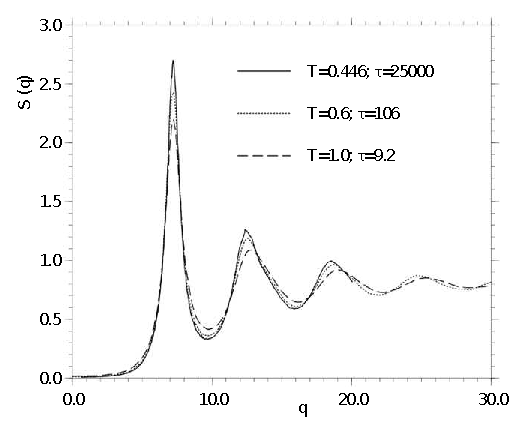
\includegraphics[width=\columnwidth]{sq_kob}
	
	\footnotesize{\citet{Kob2002}}
	
	\column{0.5\textwidth}
	While dynamics changes by 4 orders of magnitude
	\begin{itemize}
		\item Almost no change in positional order
		\item No characteristic length scale diverging toward $T_g$ or $T_0$
		\item $\neq$ critical phenomena
	\end{itemize}
	\end{columns}
\end{frame}

\begin{frame}{Fragility: super-Arrhenius behaviour}
	\begin{columns}
	\column{0.6\textwidth}
	\centering
	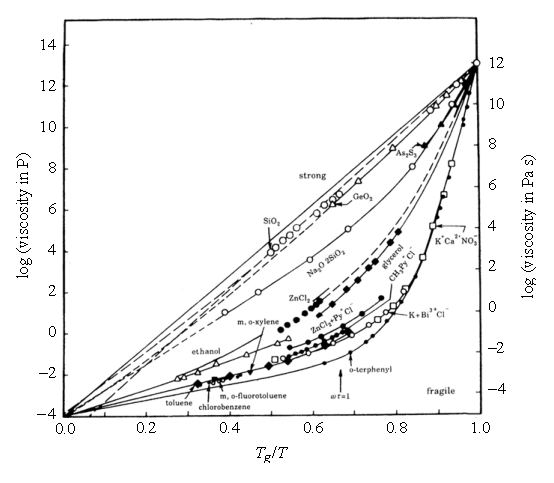
\includegraphics[width=\columnwidth]{angell}
	
	\footnotesize{\bibentry{ANGELL1988}}
	
	\column{0.4\textwidth}
	Vogel-Fulcher-Tamman empirical law:
	\[ 
	\tau = \tau_0 \exp{\left(\mathcal{D}\frac{T_0}{T_0-T}\right)}
	\]
	\begin{description}
		\setlength{\itemindent}{-4em}
		\item[$T_0$] "ideal" glass transition temperature
		\item[$\mathcal{D}$] fragility
	\end{description}
	
	\end{columns}
\end{frame}

\subsection{Dynamics of supercooled liquids}

\begin{frame}{Two step relaxation}
	\begin{columns}
	\column{0.5\textwidth}
	Self intermediate scattering function:
	\centering
	\def\svgwidth{\columnwidth}\input{isf_kob.pdf_tex}\\
	\footnotesize{\bibentry{Kob1995}}
	
	\column{0.5\textwidth}
	Supercooled liquid is ergodic
	\begin{itemize}
		\item A plateau appear
		\item $\beta$-relaxation does not change
		\item The length of the plateau changes\\ $\Rightarrow$ slowing down by many orders of magnitude
	\end{itemize}
	\end{columns}
\end{frame}

\begin{frame}{The cage theory}
	\begin{columns}
	\column{0.5\textwidth}
	\centering
	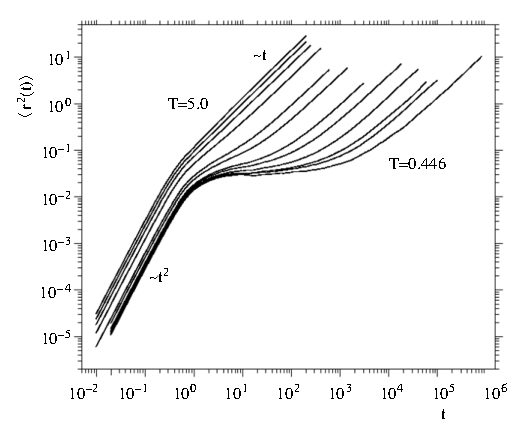
\includegraphics[width=\columnwidth]{msd_kob}
	
	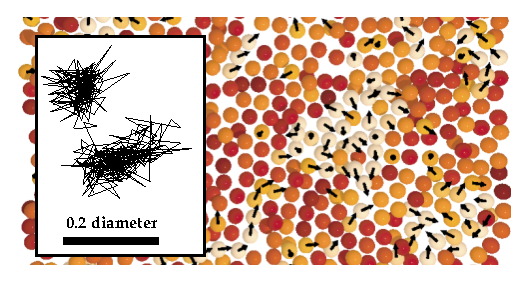
\includegraphics[width=\columnwidth]{cage_weeks}
	
	\column{0.5\textwidth}
	Mean square displacement\\
	\begin{footnotesize}\bibentry{kob1995tmc}\end{footnotesize}
	
	\bigskip
	\begin{itemize}
		\item Hopping between cages $\ll\sigma$
		\item Is the hopping probability really uniform?
	\end{itemize}
	
	\bigskip
	\begin{footnotesize}\bibentry{weeks2002pcr}\end{footnotesize}
	\end{columns}
\end{frame}

\begin{frame}{Dynamic heterogeneities}
	Fast and slow regions exist at intermediate times.
	\begin{columns}[t]
	\column{0.5\textwidth}
	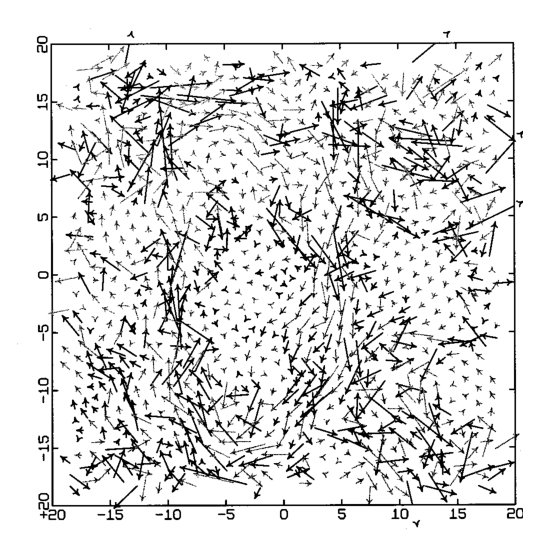
\includegraphics[width=\columnwidth]{dh_perera}
	\column{0.5\textwidth}
	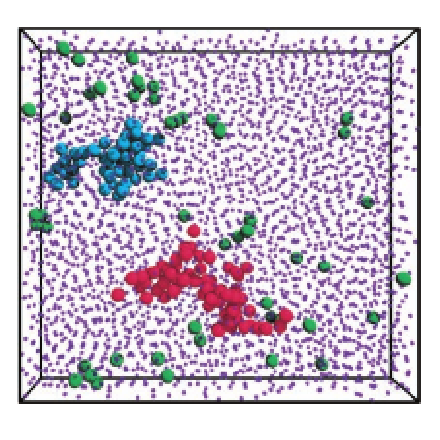
\includegraphics[width=\columnwidth]{dh_weeks}\\
	\centering{$10\%$ fastest particles}
	\end{columns}
	
	\bigskip
	\begin{footnotesize}
	\begin{columns}
	\column{0.5\textwidth}
	\bibentry{Perera1999}
	\column{0.5\textwidth}
	\bibentry{weeks2000}
	\end{columns}
	\end{footnotesize}
\end{frame}

\begin{frame}{Dynamical length scale}
	\begin{columns}
	\column{0.5\textwidth}
	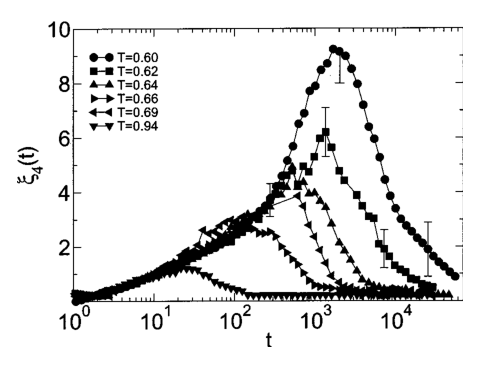
\includegraphics[width=\columnwidth]{xi4_lacevic}\\
	\begin{footnotesize}\centering\citet{Lacevic2003}\end{footnotesize}
	\column{0.5\textwidth}
	\begin{itemize}
	\item Spatial correlation of the fluctuations of the dynamics.
	\item Extract a dynamical correlation length
	\item Grows toward the glass transition
	\end{itemize}
	\end{columns}
	\begin{center}
	No statical length scale opens the door to exotic physics	
	\begin{itemize}
		\item Facilitation
		\item Space-time thermodynamics
		\item $\dots$
	\end{itemize}
	\end{center}
\end{frame}

\subsection{Quest for a static explanation?}
\begin{frame}{Static cause to dynamic heterogeneities}
	\begin{columns}
	\column{0.5\textwidth}
	\centering
	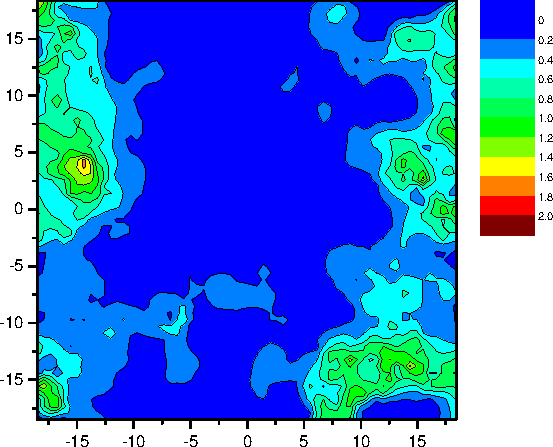
\includegraphics[width=\columnwidth]{propensity}
	\column{0.5\textwidth}
	\footnotesize{\citet{Widmer-Cooper2005}}
	\begin{itemize}
		\item $N$ runs from the same initial configuration
		\item Average out the influence of initial dynamics
		\item Propensity to displacement
		\item Predict fast/slow \alert{regions} \footnotesize{\citep{Berthier2007}}
	\end{itemize}
	\end{columns}
	
	\bigskip$\Rightarrow$ Glass transition may have a structural cause
\end{frame}

\begin{frame}{Structural cause}
	\begin{columns}
	\column{0.3\textwidth}
	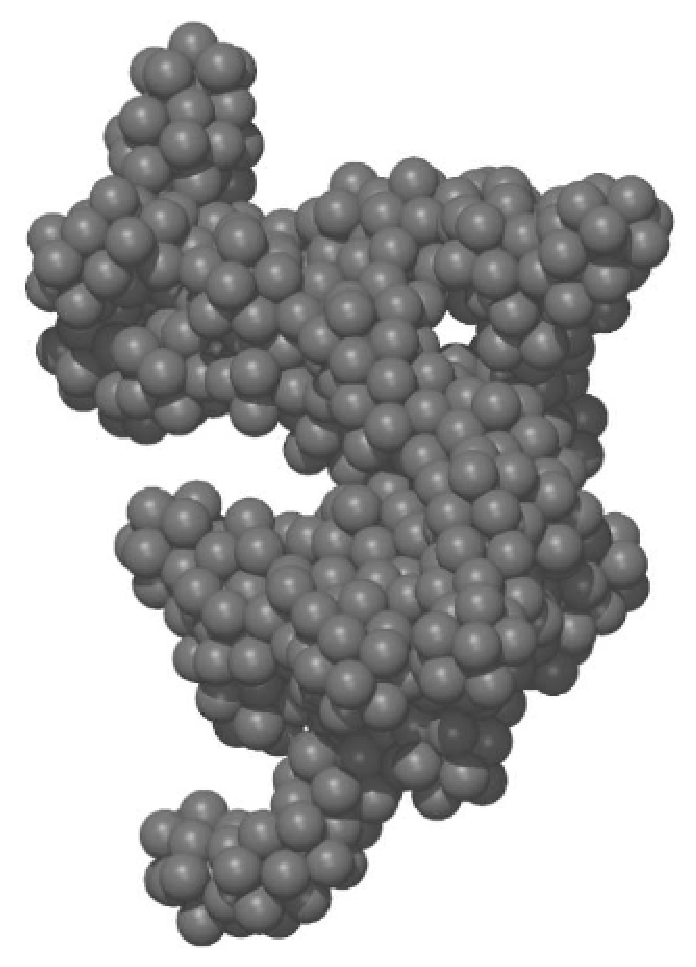
\includegraphics[width=\columnwidth]{Dzugutov_LFS}\\
	\begin{footnotesize}\citet{Dzugutov2002}\end{footnotesize}
	\column{0.5\textwidth}
	\citet{tarjus2005fba}
	\begin{itemize}
		\item Locally favoured structures
		\item Cannot fill space because of \alert{frustration}
		\item The ground state exist in
		\begin{itemize}
			\item Curved space
			\item 4 dimensions
		\end{itemize}
		\item LFS are slow		
	\end{itemize}
	\end{columns}
\end{frame}

\begin{frame}{Structural cause}
	\begin{footnotesize}\citet{tanaka2010critical}\end{footnotesize}
	\begin{columns}
	\column{0.33\textwidth}\centering
	\resizebox{\columnwidth}{!}{\input{kawa_nm_psi6.pdf_tex}}\\
	$\Psi_6$
	\column{0.33\textwidth}\centering
	\resizebox{\columnwidth}{!}{\input{kawa_nm_msd.pdf_tex}}\\
	$\Delta r^2$
	\end{columns}
	\begin{itemize}
		\item The ground state is the crystal
		\item Frustration \alert{against} crystallisation
		\begin{itemize}
			\item Other structures are locally more stable
			\item Polydispersity
		\end{itemize}
		\item Slowing down $\Leftrightarrow$ local crystal-like order
	\end{itemize}
\end{frame}

\begin{frame}{Purpose}
	\begin{itemize}
		\item Unified picture of the glass transition
		\item Quest for a static (structural) length scale diverging toward $\phi_0$
	\end{itemize}
	
	\bigskip In hard sphere colloidal supercooled liquid
	\begin{itemize}
		\item Which structure(s) is/are linked with dynamic heterogeneities?
		\item What are the relevant structures?
	\end{itemize}
\end{frame}


\section{Hard spheres colloids tracked by confocal microscopy}
\subsection{Experimental}

\begin{frame}{Hard spheres and colloids}
	\begin{textblock*}{0.6\textwidth}(10mm,92mm)
		\only<2>{\simplephasediagram{}}%
	\end{textblock*}
	The volume fraction $\phi$ is like an inverse temperature.
	\bigskip
	\def\svgwidth{\textwidth}\input{phase_diagram.pdf_tex}
	
	\bigskip
	Well approximated by sterically stabilised colloids\\
	\begin{footnotesize}\citep{pusey1986}\end{footnotesize}
\end{frame}

\begin{frame}{Our colloids}
	\begin{columns}
	\column{0.5\textwidth}
	\centering
	\rotatebox{90}{\qquad \small{SEM image}}\includegraphics[width=0.8\columnwidth]{SEM}\\
	\resizebox{\columnwidth}{!}{\begin{huge}% GNUPLOT: LaTeX picture with Postscript
\begingroup
  \makeatletter
  \providecommand\color[2][]{%
    \GenericError{(gnuplot) \space\space\space\@spaces}{%
      Package color not loaded in conjunction with
      terminal option `colourtext'%
    }{See the gnuplot documentation for explanation.%
    }{Either use 'blacktext' in gnuplot or load the package
      color.sty in LaTeX.}%
    \renewcommand\color[2][]{}%
  }%
  \providecommand\includegraphics[2][]{%
    \GenericError{(gnuplot) \space\space\space\@spaces}{%
      Package graphicx or graphics not loaded%
    }{See the gnuplot documentation for explanation.%
    }{The gnuplot epslatex terminal needs graphicx.sty or graphics.sty.}%
    \renewcommand\includegraphics[2][]{}%
  }%
  \providecommand\rotatebox[2]{#2}%
  \@ifundefined{ifGPcolor}{%
    \newif\ifGPcolor
    \GPcolortrue
  }{}%
  \@ifundefined{ifGPblacktext}{%
    \newif\ifGPblacktext
    \GPblacktexttrue
  }{}%
  % define a \g@addto@macro without @ in the name:
  \let\gplgaddtomacro\g@addto@macro
  % define empty templates for all commands taking text:
  \gdef\gplbacktext{}%
  \gdef\gplfronttext{}%
  \makeatother
  \ifGPblacktext
    % no textcolor at all
    \def\colorrgb#1{}%
    \def\colorgray#1{}%
  \else
    % gray or color?
    \ifGPcolor
      \def\colorrgb#1{\color[rgb]{#1}}%
      \def\colorgray#1{\color[gray]{#1}}%
      \expandafter\def\csname LTw\endcsname{\color{white}}%
      \expandafter\def\csname LTb\endcsname{\color{black}}%
      \expandafter\def\csname LTa\endcsname{\color{black}}%
      \expandafter\def\csname LT0\endcsname{\color[rgb]{1,0,0}}%
      \expandafter\def\csname LT1\endcsname{\color[rgb]{0,1,0}}%
      \expandafter\def\csname LT2\endcsname{\color[rgb]{0,0,1}}%
      \expandafter\def\csname LT3\endcsname{\color[rgb]{1,0,1}}%
      \expandafter\def\csname LT4\endcsname{\color[rgb]{0,1,1}}%
      \expandafter\def\csname LT5\endcsname{\color[rgb]{1,1,0}}%
      \expandafter\def\csname LT6\endcsname{\color[rgb]{0,0,0}}%
      \expandafter\def\csname LT7\endcsname{\color[rgb]{1,0.3,0}}%
      \expandafter\def\csname LT8\endcsname{\color[rgb]{0.5,0.5,0.5}}%
    \else
      % gray
      \def\colorrgb#1{\color{black}}%
      \def\colorgray#1{\color[gray]{#1}}%
      \expandafter\def\csname LTw\endcsname{\color{white}}%
      \expandafter\def\csname LTb\endcsname{\color{black}}%
      \expandafter\def\csname LTa\endcsname{\color{black}}%
      \expandafter\def\csname LT0\endcsname{\color{black}}%
      \expandafter\def\csname LT1\endcsname{\color{black}}%
      \expandafter\def\csname LT2\endcsname{\color{black}}%
      \expandafter\def\csname LT3\endcsname{\color{black}}%
      \expandafter\def\csname LT4\endcsname{\color{black}}%
      \expandafter\def\csname LT5\endcsname{\color{black}}%
      \expandafter\def\csname LT6\endcsname{\color{black}}%
      \expandafter\def\csname LT7\endcsname{\color{black}}%
      \expandafter\def\csname LT8\endcsname{\color{black}}%
    \fi
  \fi
  \setlength{\unitlength}{0.0500bp}%
  \begin{picture}(7200.00,5040.00)%
    \gplgaddtomacro\gplbacktext{%
      \csname LTb\endcsname%
      \put(1342,704){\makebox(0,0)[r]{\strut{}$0$}}%
      \put(1342,1286){\makebox(0,0)[r]{\strut{}$0.05$}}%
      \put(1342,1867){\makebox(0,0)[r]{\strut{}$0.10$}}%
      \put(1342,2449){\makebox(0,0)[r]{\strut{}$0.15$}}%
      \put(1342,3030){\makebox(0,0)[r]{\strut{}$0.20$}}%
      \put(1342,3612){\makebox(0,0)[r]{\strut{}$0.25$}}%
      \put(1342,4193){\makebox(0,0)[r]{\strut{}$0.30$}}%
      \put(1342,4775){\makebox(0,0)[r]{\strut{}$0.35$}}%
      \put(1474,484){\makebox(0,0){\strut{}$2$}}%
      \put(2148,484){\makebox(0,0){\strut{}$2.2$}}%
      \put(2823,484){\makebox(0,0){\strut{}$2.4$}}%
      \put(3497,484){\makebox(0,0){\strut{}$2.6$}}%
      \put(4172,484){\makebox(0,0){\strut{}$2.8$}}%
      \put(4846,484){\makebox(0,0){\strut{}$3$}}%
      \put(5520,484){\makebox(0,0){\strut{}$3.2$}}%
      \put(6195,484){\makebox(0,0){\strut{}$3.4$}}%
      \put(6869,484){\makebox(0,0){\strut{}$3.6$}}%
      \put(308,2739){\rotatebox{-270}{\makebox(0,0){\strut{}Probability}}}%
      \put(4171,154){\makebox(0,0){\strut{}$\sigma$ (in \micro\meter)}}%
    }%
    \gplgaddtomacro\gplfronttext{%
    }%
    \gplbacktext
    \put(0,0){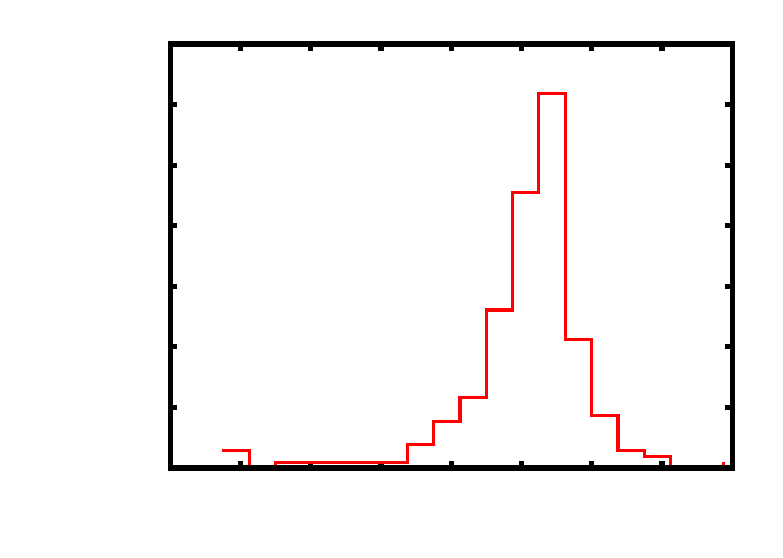
\includegraphics{diameter_histogram}}%
    \gplfronttext
  \end{picture}%
\endgroup
\end{huge}}
	\column{0.5\textwidth}
	\begin{itemize}
		\item PMMA particles 
		\begin{itemize}
			\item $\sigma \simeq \unit{3.3}{\micro\metre}$
			\item $\Delta \simeq 6\%$ not Gaussian
		\end{itemize}
		\item Hard spheres
		\begin{itemize}
			\item Sterically stabilized
			\item Salt to screen charges\\ (Debye length $<\unit{100}{\nano}{\metre}$)
		\end{itemize}
		\item Solvent
		\begin{itemize}
			\item Cis-decalin
			\item Cyclohexylbromide
		\end{itemize}
		\item Matching
		\begin{itemize}
			\item Optical index
			\item Density (with $T$ control)
		\end{itemize}
	\end{itemize}
	\end{columns}
\end{frame}

\begin{frame}{Confocal microscopy}
	\begin{columns}
	\column{0.4\textwidth}
	\def\svgwidth{\columnwidth}\input{confocalprinciple_vertical.pdf_tex}
	\column{0.6\textwidth}
	\centering
	$XY$ slice\quad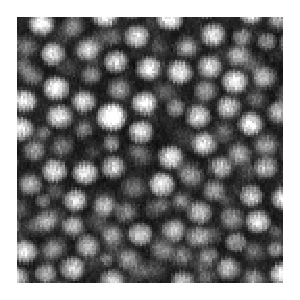
\includegraphics[width=0.5\columnwidth]{sliceXY}  
	
	\bigskip
	$XZ$ slice\quad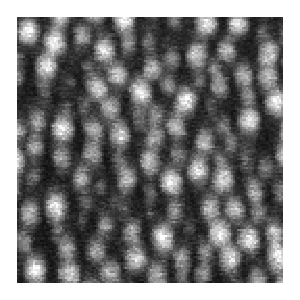
\includegraphics[width=0.5\columnwidth]{sliceXZ}
	\end{columns}
\end{frame}

\subsection{Tracking}
\begin{frame}{Particle tracking}
	\begin{columns}[T]
	\column{0.3\textwidth}
	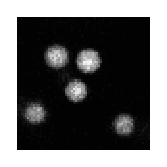
\includegraphics[width=\textwidth]{dillute_raw}
	
	\bigskip
	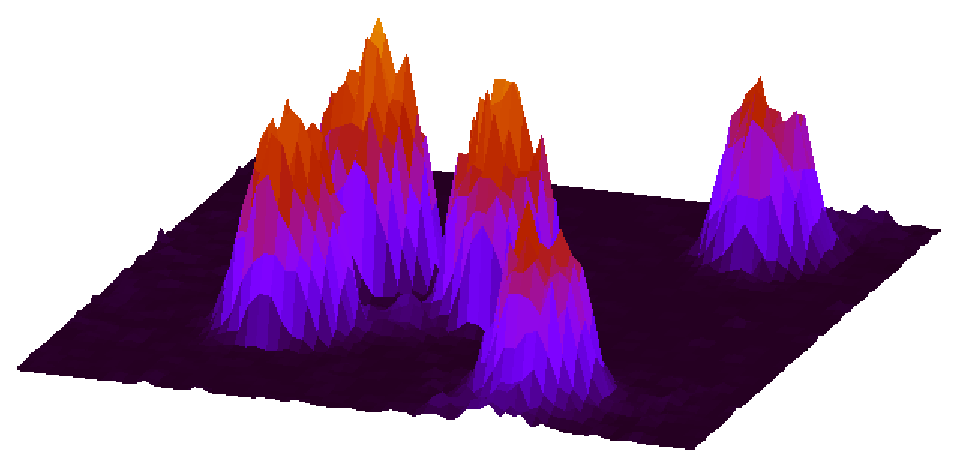
\includegraphics[width=\textwidth]{dillute_raw_gp_raster}
	\column{0.3\textwidth}
	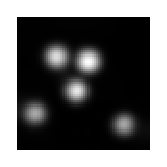
\includegraphics[width=\textwidth]{dillute_filtered}
	
	\bigskip
	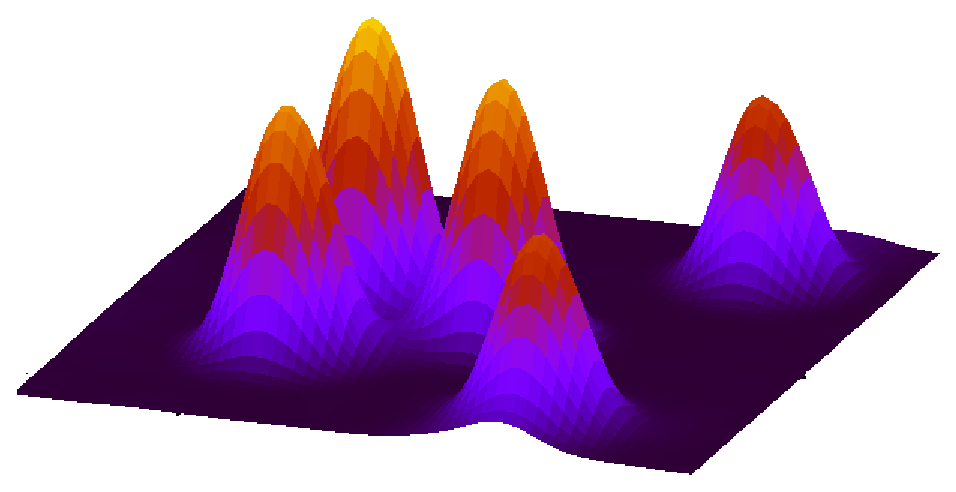
\includegraphics[width=\textwidth]{dillute_filtered_gp_raster}
	\column{0.3\textwidth}
	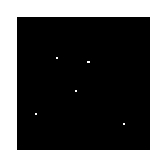
\includegraphics[width=\textwidth]{dillute_centers}
	
	\bigskip
	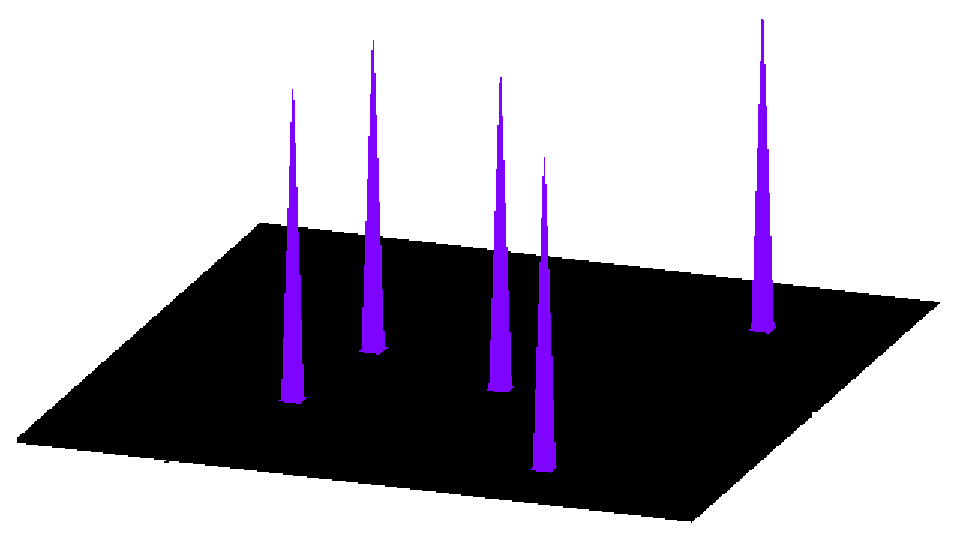
\includegraphics[width=\textwidth]{dillute_centers_gp_raster}
	\end{columns}
	
	\bigskip
	\[ (\unit{512}{pixels})^3 \xrightarrow{\unit{4}{\second}} \unit{5\times 10^4}{particles} \]
\end{frame}

\begin{frame}{Tracking accuracy}
	\begin{columns}
	\column{0.7\textwidth}
	\only<1|handout:0>{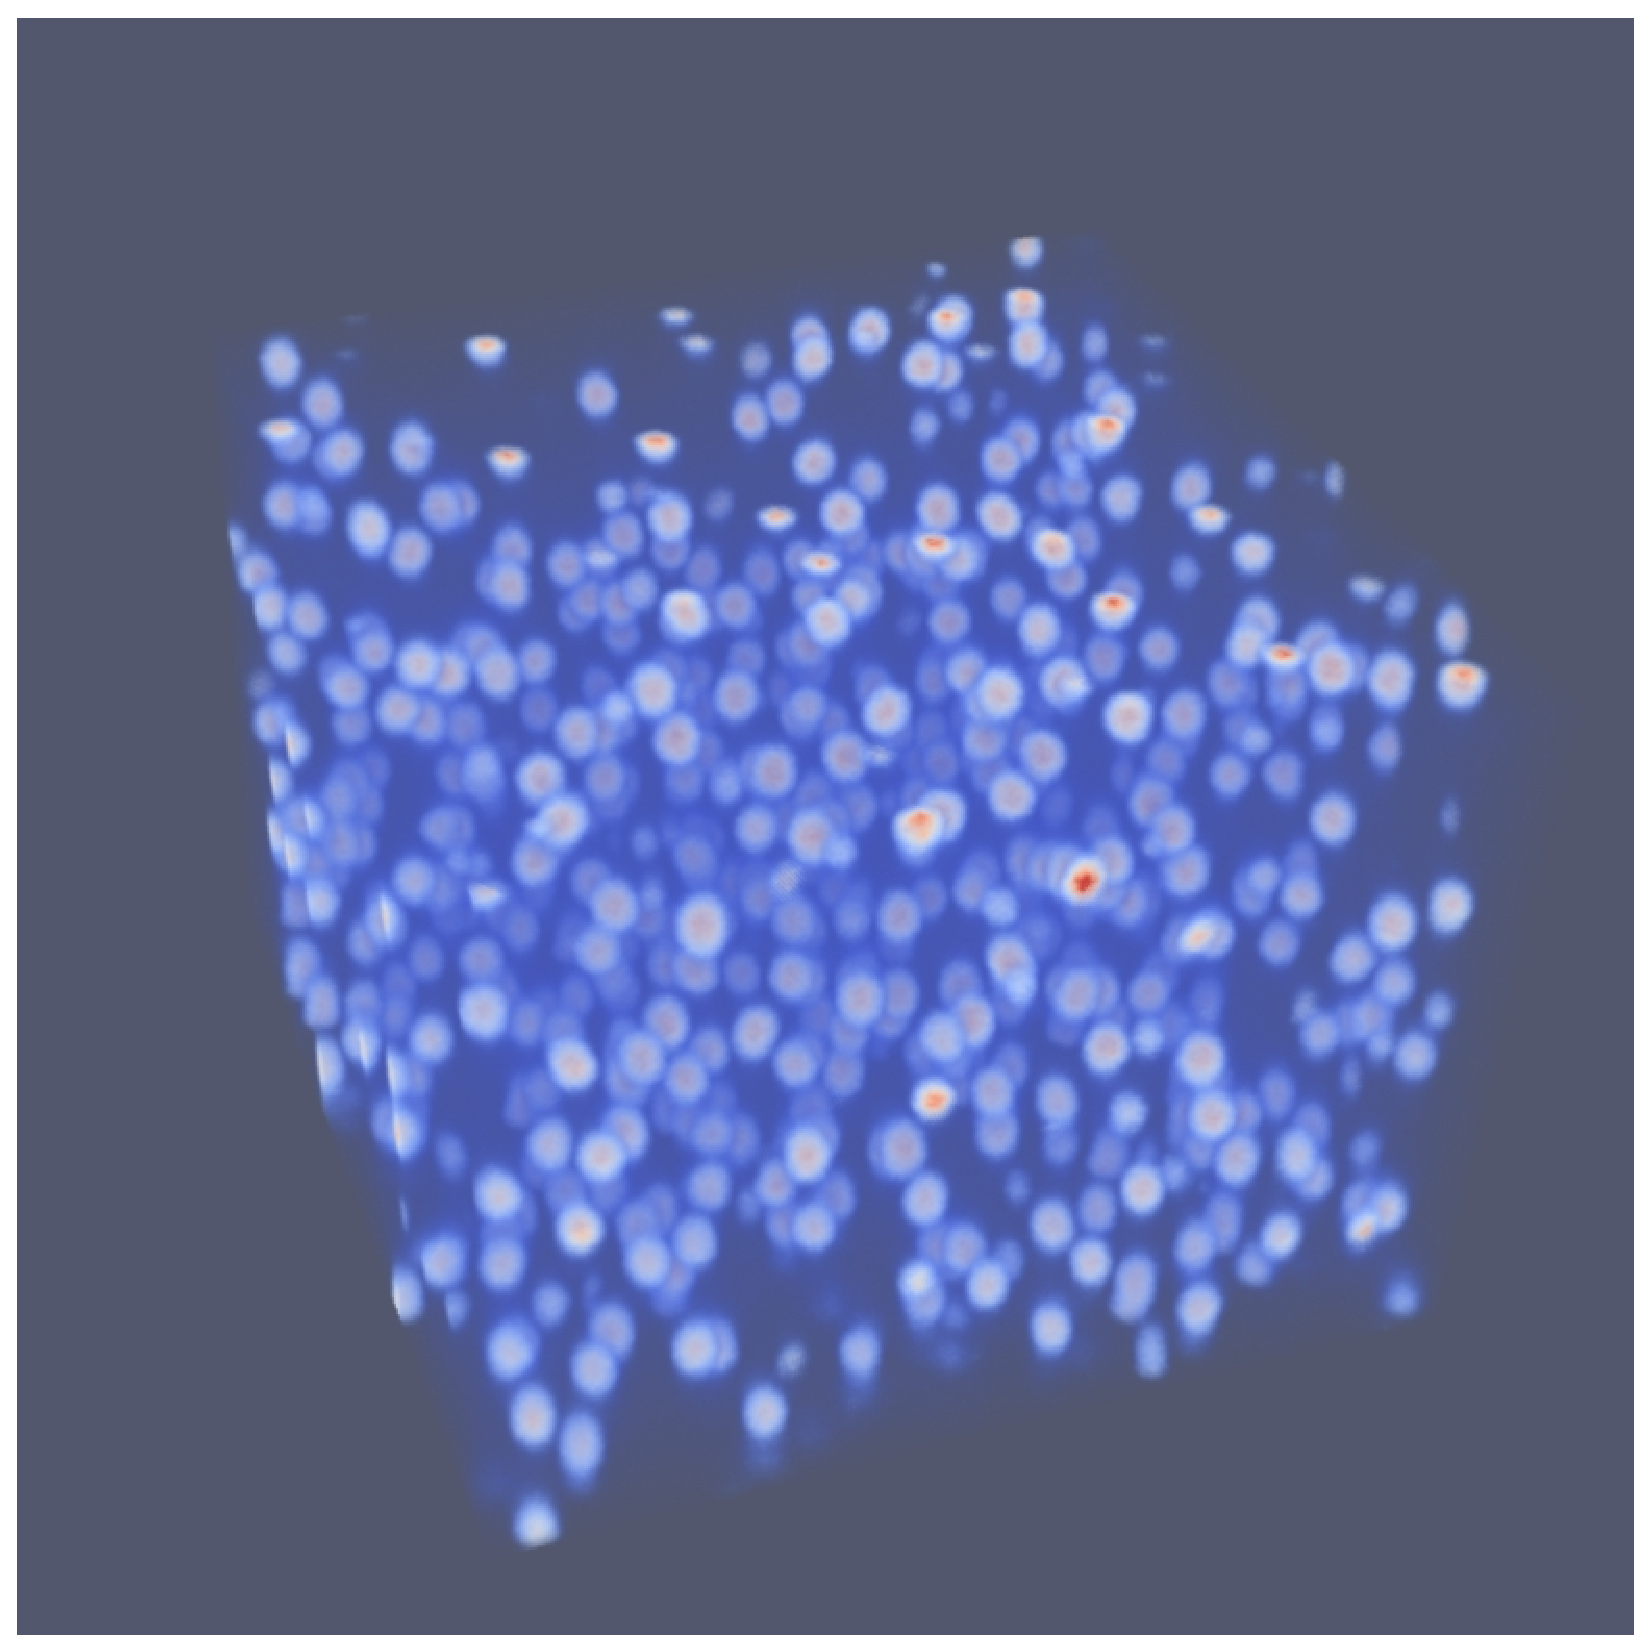
\includegraphics[width=\columnwidth]{compare_image_tracked3D_0}}%
	\only<2|handout:0>{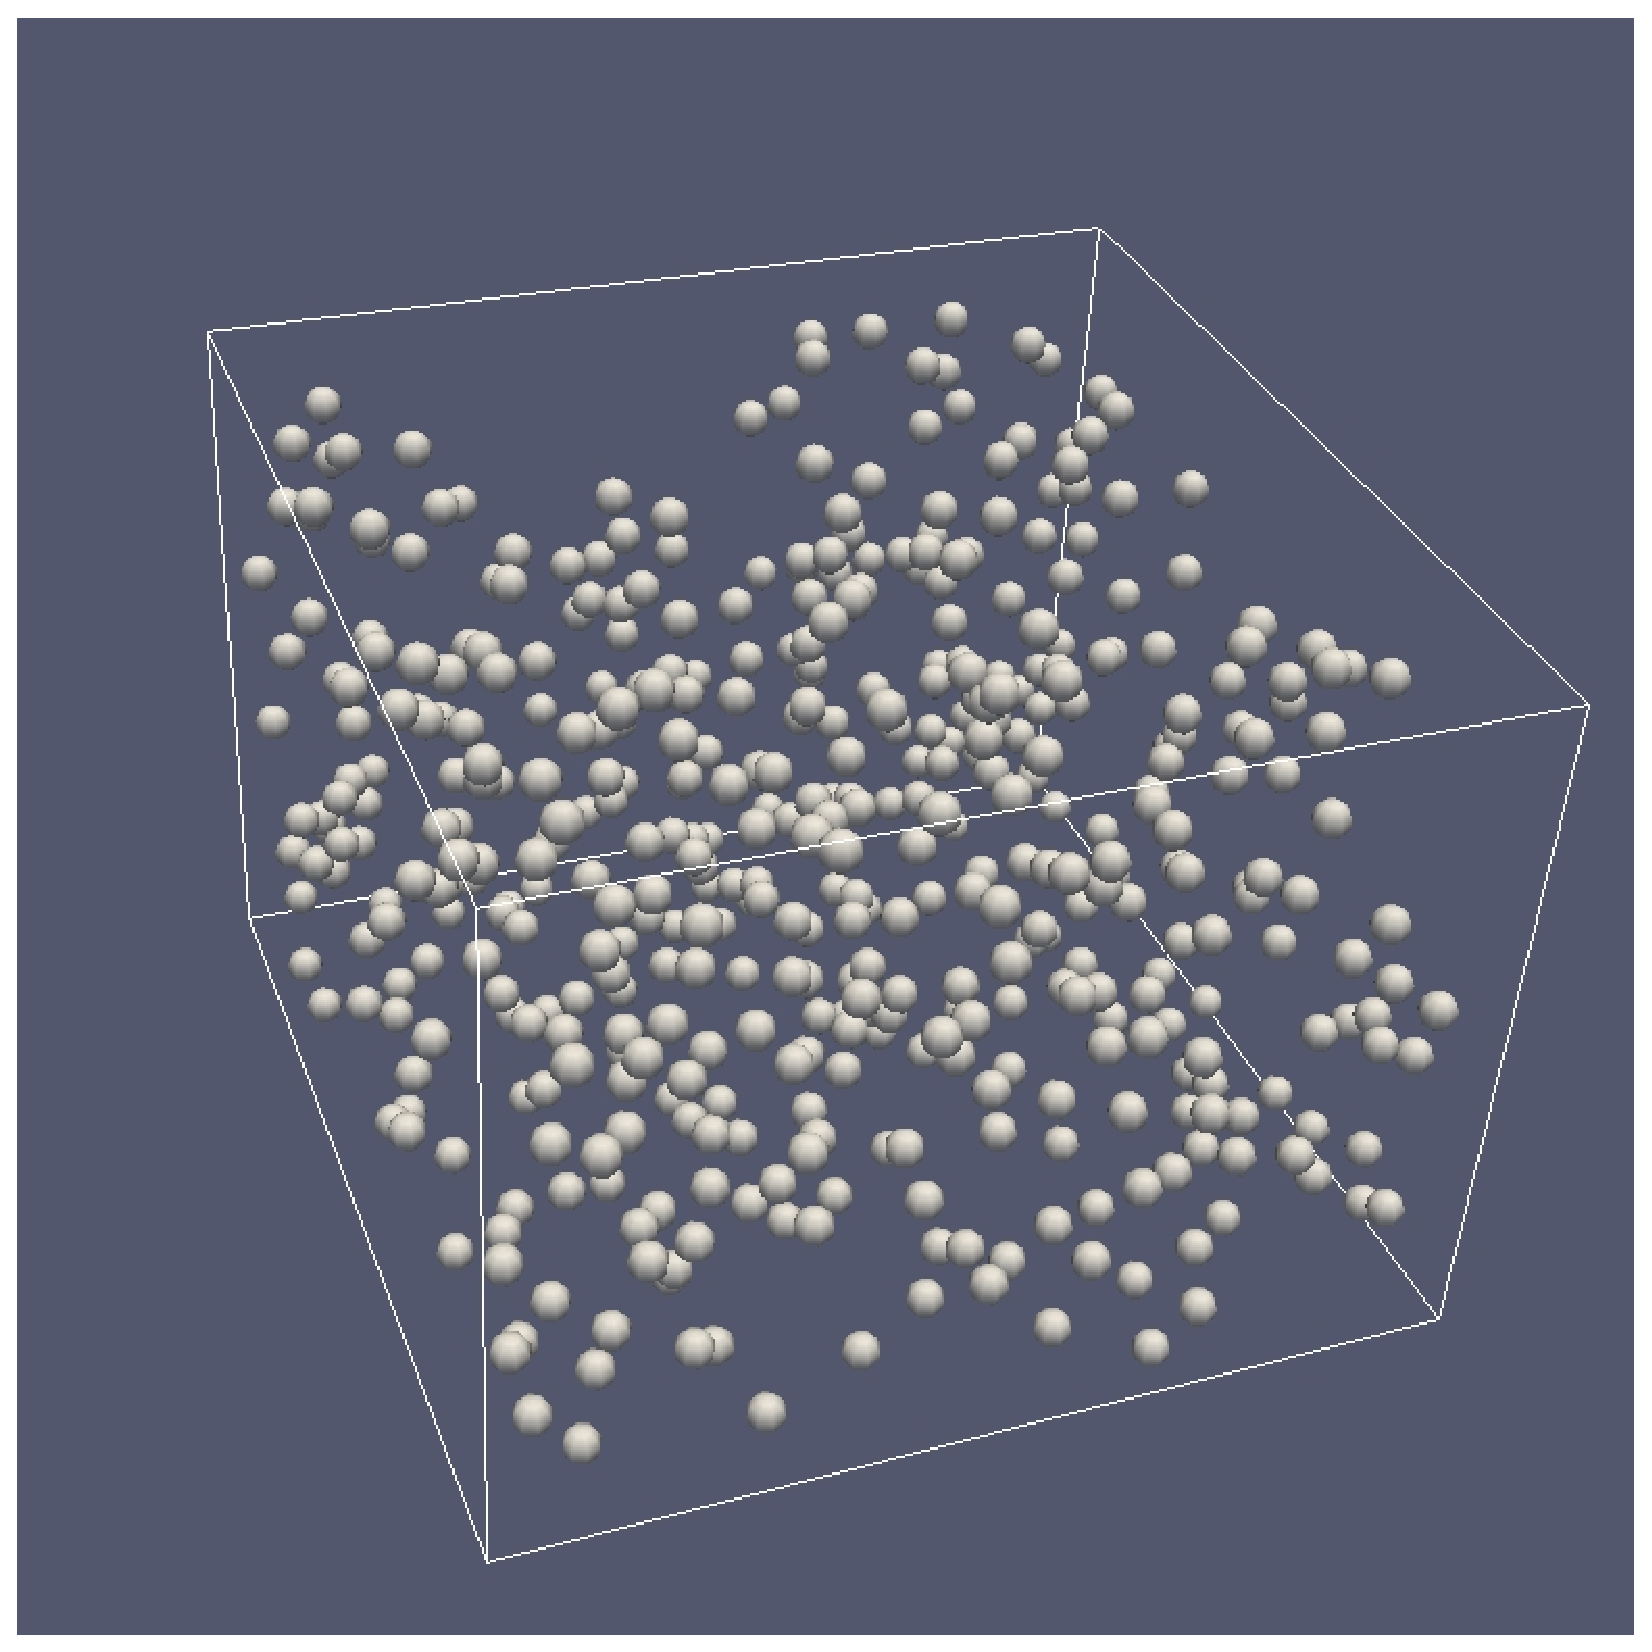
\includegraphics[width=\columnwidth]{compare_image_tracked3D_1}}%
	\only<3>{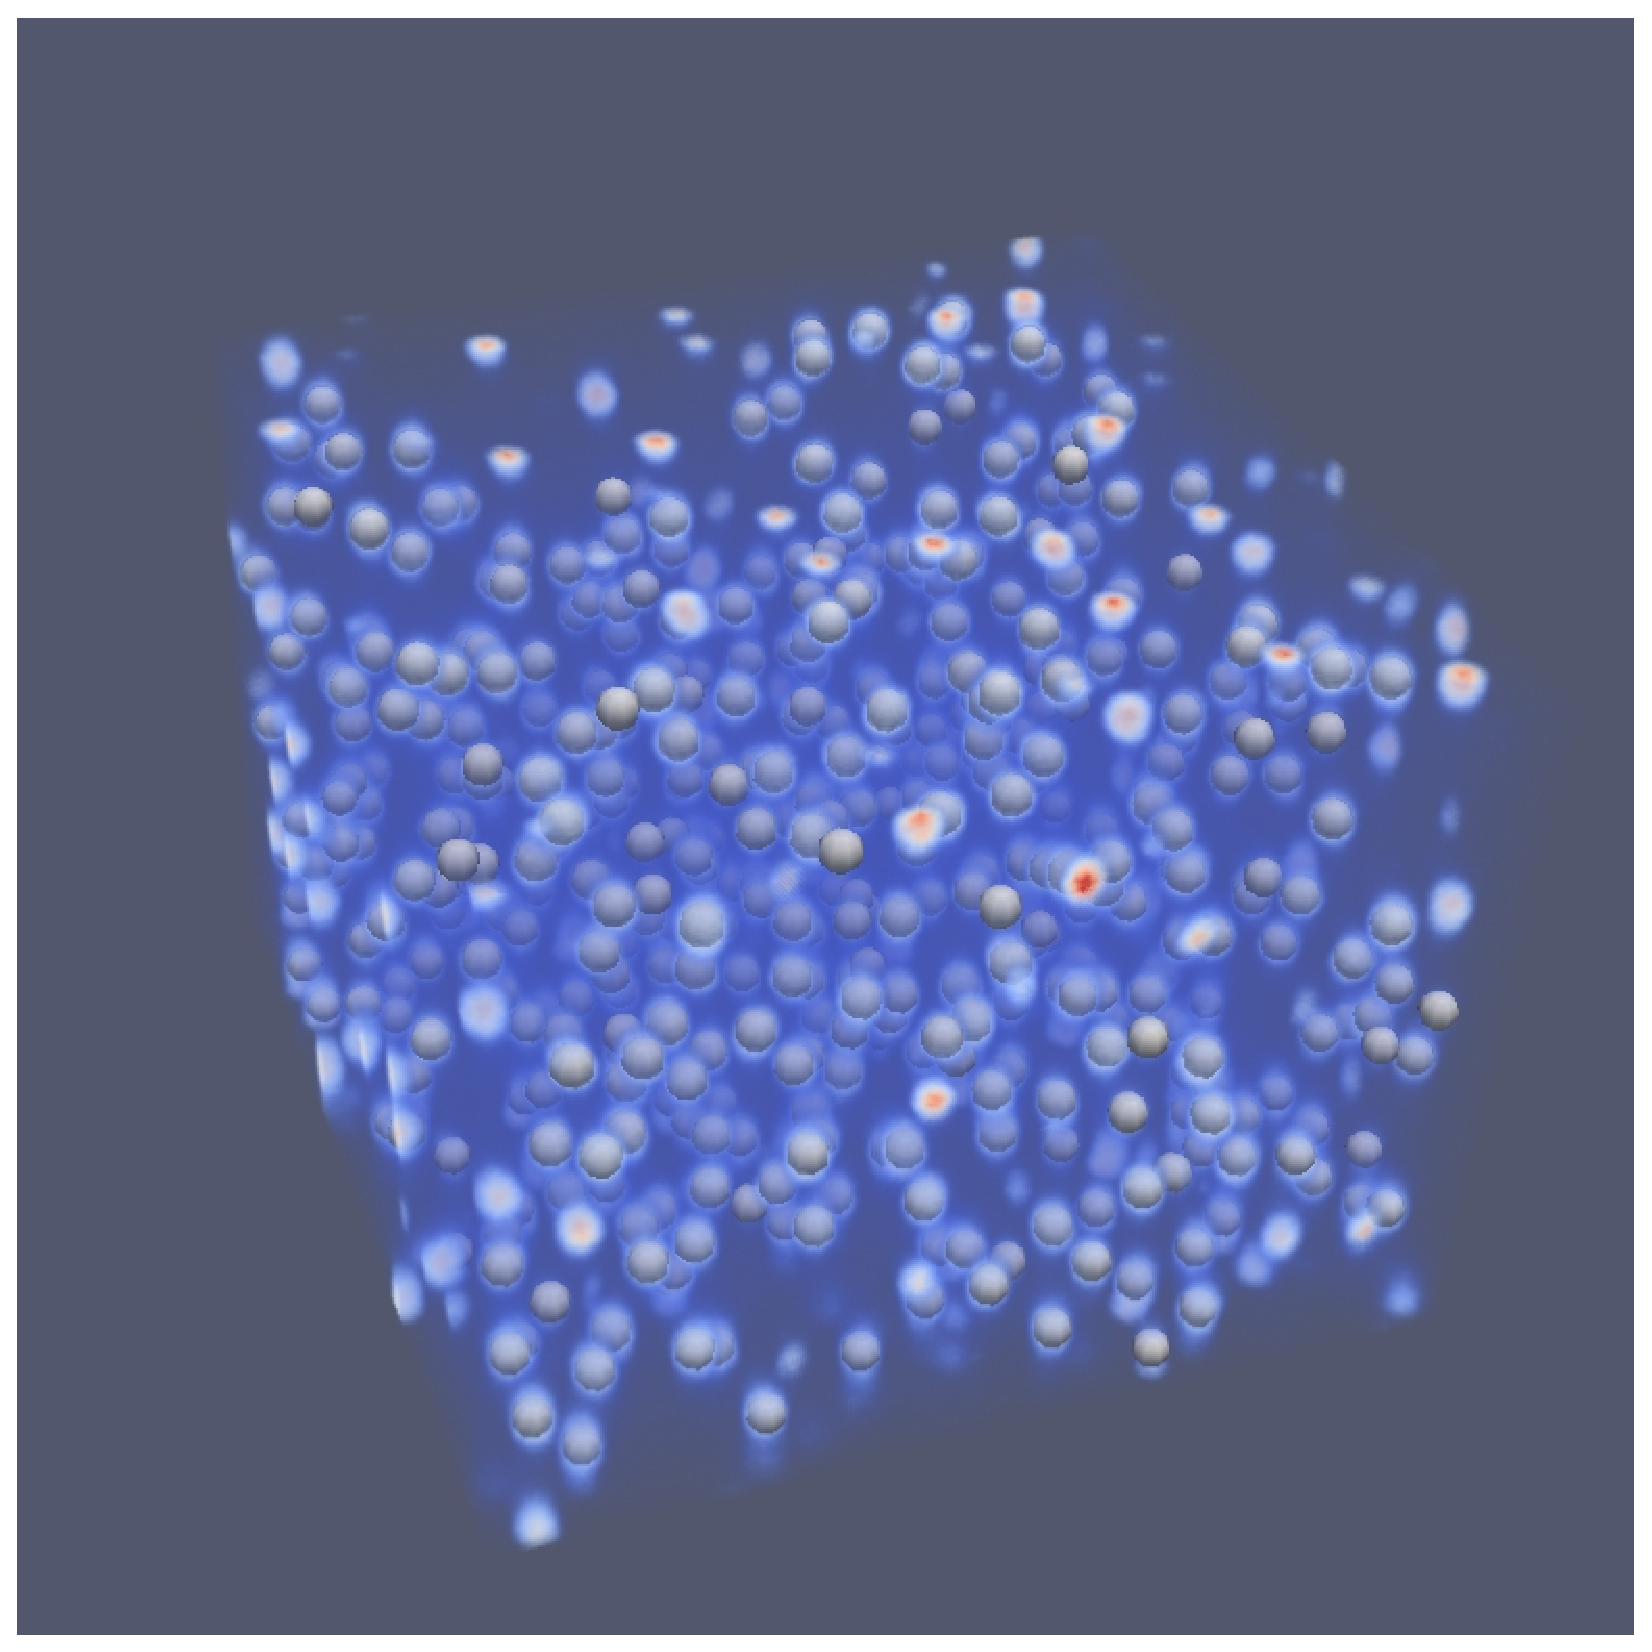
\includegraphics[width=\columnwidth]{compare_image_tracked3D_2}}\\
	\centering{\uncover<1,3>{Image}\uncover<3>{ $+$ }\uncover<2,3>{Tracked}}
	\column{0.3\textwidth}
	\begin{itemize}
		\item All particles are tracked
		\item Only particles are tracked
		\item Precision is about
	\end{itemize}
	\begin{align*}
		&\unit{0.1}{pixels}\\
		&\unit{0.01}{\sigma}\\
		&\unit{30}{\nano\metre}
	\end{align*}
	\end{columns}
\end{frame}

\subsection{Simulations}

\begin{frame}{Comparing with Brownian dynamics simulations}
	\begin{columns}
	\column{0.4\textwidth}
		\resizebox{\columnwidth}{!}{\begin{Large}% GNUPLOT: LaTeX picture with Postscript
\begingroup
  \makeatletter
  \providecommand\color[2][]{%
    \GenericError{(gnuplot) \space\space\space\@spaces}{%
      Package color not loaded in conjunction with
      terminal option `colourtext'%
    }{See the gnuplot documentation for explanation.%
    }{Either use 'blacktext' in gnuplot or load the package
      color.sty in LaTeX.}%
    \renewcommand\color[2][]{}%
  }%
  \providecommand\includegraphics[2][]{%
    \GenericError{(gnuplot) \space\space\space\@spaces}{%
      Package graphicx or graphics not loaded%
    }{See the gnuplot documentation for explanation.%
    }{The gnuplot epslatex terminal needs graphicx.sty or graphics.sty.}%
    \renewcommand\includegraphics[2][]{}%
  }%
  \providecommand\rotatebox[2]{#2}%
  \@ifundefined{ifGPcolor}{%
    \newif\ifGPcolor
    \GPcolortrue
  }{}%
  \@ifundefined{ifGPblacktext}{%
    \newif\ifGPblacktext
    \GPblacktexttrue
  }{}%
  % define a \g@addto@macro without @ in the name:
  \let\gplgaddtomacro\g@addto@macro
  % define empty templates for all commands taking text:
  \gdef\gplbacktext{}%
  \gdef\gplfronttext{}%
  \makeatother
  \ifGPblacktext
    % no textcolor at all
    \def\colorrgb#1{}%
    \def\colorgray#1{}%
  \else
    % gray or color?
    \ifGPcolor
      \def\colorrgb#1{\color[rgb]{#1}}%
      \def\colorgray#1{\color[gray]{#1}}%
      \expandafter\def\csname LTw\endcsname{\color{white}}%
      \expandafter\def\csname LTb\endcsname{\color{black}}%
      \expandafter\def\csname LTa\endcsname{\color{black}}%
      \expandafter\def\csname LT0\endcsname{\color[rgb]{1,0,0}}%
      \expandafter\def\csname LT1\endcsname{\color[rgb]{0,1,0}}%
      \expandafter\def\csname LT2\endcsname{\color[rgb]{0,0,1}}%
      \expandafter\def\csname LT3\endcsname{\color[rgb]{1,0,1}}%
      \expandafter\def\csname LT4\endcsname{\color[rgb]{0,1,1}}%
      \expandafter\def\csname LT5\endcsname{\color[rgb]{1,1,0}}%
      \expandafter\def\csname LT6\endcsname{\color[rgb]{0,0,0}}%
      \expandafter\def\csname LT7\endcsname{\color[rgb]{1,0.3,0}}%
      \expandafter\def\csname LT8\endcsname{\color[rgb]{0.5,0.5,0.5}}%
    \else
      % gray
      \def\colorrgb#1{\color{black}}%
      \def\colorgray#1{\color[gray]{#1}}%
      \expandafter\def\csname LTw\endcsname{\color{white}}%
      \expandafter\def\csname LTb\endcsname{\color{black}}%
      \expandafter\def\csname LTa\endcsname{\color{black}}%
      \expandafter\def\csname LT0\endcsname{\color{black}}%
      \expandafter\def\csname LT1\endcsname{\color{black}}%
      \expandafter\def\csname LT2\endcsname{\color{black}}%
      \expandafter\def\csname LT3\endcsname{\color{black}}%
      \expandafter\def\csname LT4\endcsname{\color{black}}%
      \expandafter\def\csname LT5\endcsname{\color{black}}%
      \expandafter\def\csname LT6\endcsname{\color{black}}%
      \expandafter\def\csname LT7\endcsname{\color{black}}%
      \expandafter\def\csname LT8\endcsname{\color{black}}%
    \fi
  \fi
  \setlength{\unitlength}{0.0500bp}%
  \begin{picture}(3600.00,5040.00)%
    \gplgaddtomacro\gplbacktext{%
      \csname LTb\endcsname%
      \put(660,704){\makebox(0,0)[r]{\strut{}$0$}}%
      \put(660,2740){\makebox(0,0)[r]{\strut{}$0.025$}}%
      \put(660,4776){\makebox(0,0)[r]{\strut{}$0.05$}}%
      \put(1266,484){\makebox(0,0){\strut{}$1$}}%
      \put(2213,484){\makebox(0,0){\strut{}$1.1$}}%
      \put(3160,484){\makebox(0,0){\strut{}$1.2$}}%
      \put(418,3840){\rotatebox{-270}{\makebox(0,0){\strut{}$U(r)/\epsilon$}}}%
      \put(3379,2740){\rotatebox{-270}{\makebox(0,0){\strut{}}}}%
      \put(1976,154){\makebox(0,0){\strut{}$r/\sigma$}}%
      \put(1976,4666){\makebox(0,0){\strut{}}}%
      \put(1976,4665){\makebox(0,0){\strut{}}}%
      \put(-396,110){\makebox(0,0)[l]{\strut{}}}%
      \put(1502,3147){\makebox(0,0){\strut{}$\frac{k_B T}{\epsilon}$}}%
      \put(2118,1722){\makebox(0,0)[r]{\strut{}$\sigma_{eff}$}}%
    }%
    \gplgaddtomacro\gplfronttext{%
    }%
    \gplbacktext
    \put(0,0){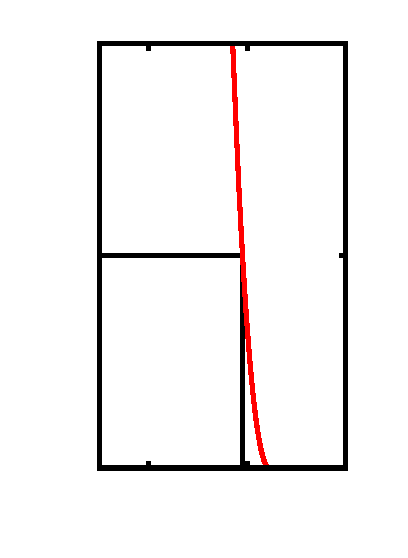
\includegraphics{wca}}%
    \gplfronttext
  \end{picture}%
\endgroup
\end{Large}}
	\column{0.6\textwidth}
	\begin{itemize}
		\item WCA potential: quasi hard-spheres
	\end{itemize}
	\[ U_{jk}(r) = \left\{\begin{array}{l l}
  		4\epsilon & \left[ \left( \frac{\sigma_{jk}}{r}\right)^{12} - \left( \frac{\sigma_{jk}}{r}\right)^{6} +\frac{1}{4}\right]  \\
  		& \quad \text{for }r<2^\frac{1}{6} \sigma_{jk}\\
  		0 & \quad \text{otherwise}
  	\end{array} \right. \]
  	\begin{itemize}
		\item Brownian $\simeq$ colloidal
		\item Gaussian polydispersity $\Delta=6\%$
		\item Periodic boundary conditions
	\end{itemize}
	
	\bigskip
	\footnotesize{Re-analysing simulations of Takeshi Kawasaki}
	\end{columns}
\end{frame}

\subsection{Dynamic signature}

\begin{frame}{Dynamic signature}
	\begin{columns}[T]
	\column{0.5\textwidth}
	\alt<1|handout:0>{\resizebox{\columnwidth}{0.7\columnwidth}{\input{isf_kob.pdf_tex}}}%
		{\resizebox{\textwidth}{!}{\begin{Large}% GNUPLOT: LaTeX picture with Postscript
\begingroup
  \makeatletter
  \providecommand\color[2][]{%
    \GenericError{(gnuplot) \space\space\space\@spaces}{%
      Package color not loaded in conjunction with
      terminal option `colourtext'%
    }{See the gnuplot documentation for explanation.%
    }{Either use 'blacktext' in gnuplot or load the package
      color.sty in LaTeX.}%
    \renewcommand\color[2][]{}%
  }%
  \providecommand\includegraphics[2][]{%
    \GenericError{(gnuplot) \space\space\space\@spaces}{%
      Package graphicx or graphics not loaded%
    }{See the gnuplot documentation for explanation.%
    }{The gnuplot epslatex terminal needs graphicx.sty or graphics.sty.}%
    \renewcommand\includegraphics[2][]{}%
  }%
  \providecommand\rotatebox[2]{#2}%
  \@ifundefined{ifGPcolor}{%
    \newif\ifGPcolor
    \GPcolortrue
  }{}%
  \@ifundefined{ifGPblacktext}{%
    \newif\ifGPblacktext
    \GPblacktexttrue
  }{}%
  % define a \g@addto@macro without @ in the name:
  \let\gplgaddtomacro\g@addto@macro
  % define empty templates for all commands taking text:
  \gdef\gplbacktext{}%
  \gdef\gplfronttext{}%
  \makeatother
  \ifGPblacktext
    % no textcolor at all
    \def\colorrgb#1{}%
    \def\colorgray#1{}%
  \else
    % gray or color?
    \ifGPcolor
      \def\colorrgb#1{\color[rgb]{#1}}%
      \def\colorgray#1{\color[gray]{#1}}%
      \expandafter\def\csname LTw\endcsname{\color{white}}%
      \expandafter\def\csname LTb\endcsname{\color{black}}%
      \expandafter\def\csname LTa\endcsname{\color{black}}%
      \expandafter\def\csname LT0\endcsname{\color[rgb]{1,0,0}}%
      \expandafter\def\csname LT1\endcsname{\color[rgb]{0,1,0}}%
      \expandafter\def\csname LT2\endcsname{\color[rgb]{0,0,1}}%
      \expandafter\def\csname LT3\endcsname{\color[rgb]{1,0,1}}%
      \expandafter\def\csname LT4\endcsname{\color[rgb]{0,1,1}}%
      \expandafter\def\csname LT5\endcsname{\color[rgb]{1,1,0}}%
      \expandafter\def\csname LT6\endcsname{\color[rgb]{0,0,0}}%
      \expandafter\def\csname LT7\endcsname{\color[rgb]{1,0.3,0}}%
      \expandafter\def\csname LT8\endcsname{\color[rgb]{0.5,0.5,0.5}}%
    \else
      % gray
      \def\colorrgb#1{\color{black}}%
      \def\colorgray#1{\color[gray]{#1}}%
      \expandafter\def\csname LTw\endcsname{\color{white}}%
      \expandafter\def\csname LTb\endcsname{\color{black}}%
      \expandafter\def\csname LTa\endcsname{\color{black}}%
      \expandafter\def\csname LT0\endcsname{\color{black}}%
      \expandafter\def\csname LT1\endcsname{\color{black}}%
      \expandafter\def\csname LT2\endcsname{\color{black}}%
      \expandafter\def\csname LT3\endcsname{\color{black}}%
      \expandafter\def\csname LT4\endcsname{\color{black}}%
      \expandafter\def\csname LT5\endcsname{\color{black}}%
      \expandafter\def\csname LT6\endcsname{\color{black}}%
      \expandafter\def\csname LT7\endcsname{\color{black}}%
      \expandafter\def\csname LT8\endcsname{\color{black}}%
    \fi
  \fi
  \setlength{\unitlength}{0.0500bp}%
  \begin{picture}(7200.00,5040.00)%
    \gplgaddtomacro\gplbacktext{%
      \csname LTb\endcsname%
      \put(1056,1518){\makebox(0,0)[r]{\strut{}$0.2$}}%
      \put(1056,2333){\makebox(0,0)[r]{\strut{}$0.4$}}%
      \put(1056,3147){\makebox(0,0)[r]{\strut{}$0.6$}}%
      \put(1056,3962){\makebox(0,0)[r]{\strut{}$0.8$}}%
      \put(1056,4776){\makebox(0,0)[r]{\strut{}$1$}}%
      \put(1251,484){\makebox(0,0){\strut{}$10^{0}$}}%
      \put(2628,484){\makebox(0,0){\strut{}$10^{1}$}}%
      \put(4006,484){\makebox(0,0){\strut{}$10^{2}$}}%
      \put(5383,484){\makebox(0,0){\strut{}$10^{3}$}}%
      \put(6760,484){\makebox(0,0){\strut{}$10^{4}$}}%
      \put(418,2740){\rotatebox{-270}{\makebox(0,0){\strut{}Self \ac{ISF}}}}%
      \put(6979,2740){\rotatebox{-270}{\makebox(0,0){\strut{}}}}%
      \put(3974,154){\makebox(0,0){\strut{}$t/\tau_B$}}%
      \put(3974,4666){\makebox(0,0){\strut{}}}%
      \put(3974,4665){\makebox(0,0){\strut{}}}%
      \put(264,110){\makebox(0,0)[l]{\strut{}}}%
    }%
    \gplgaddtomacro\gplfronttext{%
      \csname LTb\endcsname%
      \put(6037,3525){\makebox(0,0)[r]{\strut{}$\phi=0.497$}}%
      \csname LTb\endcsname%
      \put(6037,3789){\makebox(0,0)[r]{\strut{}$\phi=0.535$}}%
      \csname LTb\endcsname%
      \put(6037,4053){\makebox(0,0)[r]{\strut{}$\phi=0.540$}}%
      \csname LTb\endcsname%
      \put(6037,4317){\makebox(0,0)[r]{\strut{}$\phi=0.555$}}%
      \csname LTb\endcsname%
      \put(6037,4581){\makebox(0,0)[r]{\strut{}$\phi=0.576$}}%
    }%
    \gplbacktext
    \put(0,0){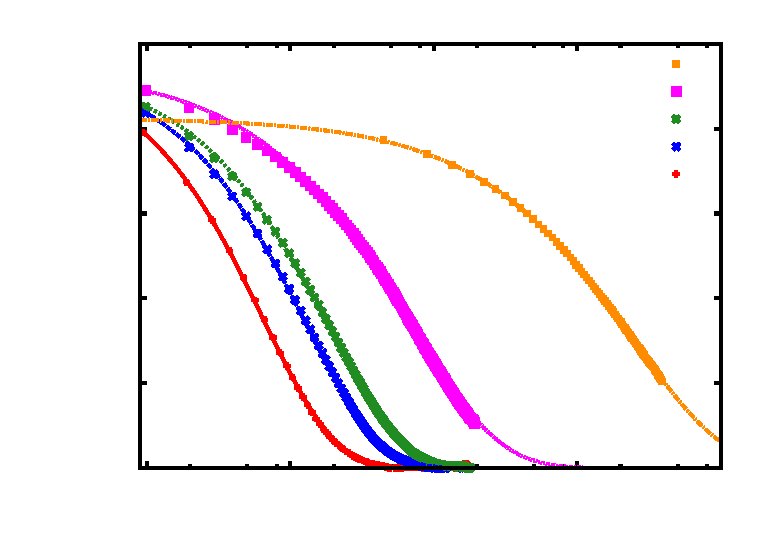
\includegraphics{./fit_isf}}%
    \gplfronttext
  \end{picture}%
\endgroup
\end{Large}}}%
	\begin{itemize}
		\item Dramatic slowing down
		\item Two step relaxation
		\item Plateau
		\item VFT fit $\Rightarrow\phi_0$
		\item<4> Good agreement with simulations
	\end{itemize}
	\column{0.5\textwidth}
	\alt<3->{\resizebox{\textwidth}{!}{\begin{Large}% GNUPLOT: LaTeX picture with Postscript
\begingroup
  \makeatletter
  \providecommand\color[2][]{%
    \GenericError{(gnuplot) \space\space\space\@spaces}{%
      Package color not loaded in conjunction with
      terminal option `colourtext'%
    }{See the gnuplot documentation for explanation.%
    }{Either use 'blacktext' in gnuplot or load the package
      color.sty in LaTeX.}%
    \renewcommand\color[2][]{}%
  }%
  \providecommand\includegraphics[2][]{%
    \GenericError{(gnuplot) \space\space\space\@spaces}{%
      Package graphicx or graphics not loaded%
    }{See the gnuplot documentation for explanation.%
    }{The gnuplot epslatex terminal needs graphicx.sty or graphics.sty.}%
    \renewcommand\includegraphics[2][]{}%
  }%
  \providecommand\rotatebox[2]{#2}%
  \@ifundefined{ifGPcolor}{%
    \newif\ifGPcolor
    \GPcolortrue
  }{}%
  \@ifundefined{ifGPblacktext}{%
    \newif\ifGPblacktext
    \GPblacktexttrue
  }{}%
  % define a \g@addto@macro without @ in the name:
  \let\gplgaddtomacro\g@addto@macro
  % define empty templates for all commands taking text:
  \gdef\gplbacktext{}%
  \gdef\gplfronttext{}%
  \makeatother
  \ifGPblacktext
    % no textcolor at all
    \def\colorrgb#1{}%
    \def\colorgray#1{}%
  \else
    % gray or color?
    \ifGPcolor
      \def\colorrgb#1{\color[rgb]{#1}}%
      \def\colorgray#1{\color[gray]{#1}}%
      \expandafter\def\csname LTw\endcsname{\color{white}}%
      \expandafter\def\csname LTb\endcsname{\color{black}}%
      \expandafter\def\csname LTa\endcsname{\color{black}}%
      \expandafter\def\csname LT0\endcsname{\color[rgb]{1,0,0}}%
      \expandafter\def\csname LT1\endcsname{\color[rgb]{0,1,0}}%
      \expandafter\def\csname LT2\endcsname{\color[rgb]{0,0,1}}%
      \expandafter\def\csname LT3\endcsname{\color[rgb]{1,0,1}}%
      \expandafter\def\csname LT4\endcsname{\color[rgb]{0,1,1}}%
      \expandafter\def\csname LT5\endcsname{\color[rgb]{1,1,0}}%
      \expandafter\def\csname LT6\endcsname{\color[rgb]{0,0,0}}%
      \expandafter\def\csname LT7\endcsname{\color[rgb]{1,0.3,0}}%
      \expandafter\def\csname LT8\endcsname{\color[rgb]{0.5,0.5,0.5}}%
    \else
      % gray
      \def\colorrgb#1{\color{black}}%
      \def\colorgray#1{\color[gray]{#1}}%
      \expandafter\def\csname LTw\endcsname{\color{white}}%
      \expandafter\def\csname LTb\endcsname{\color{black}}%
      \expandafter\def\csname LTa\endcsname{\color{black}}%
      \expandafter\def\csname LT0\endcsname{\color{black}}%
      \expandafter\def\csname LT1\endcsname{\color{black}}%
      \expandafter\def\csname LT2\endcsname{\color{black}}%
      \expandafter\def\csname LT3\endcsname{\color{black}}%
      \expandafter\def\csname LT4\endcsname{\color{black}}%
      \expandafter\def\csname LT5\endcsname{\color{black}}%
      \expandafter\def\csname LT6\endcsname{\color{black}}%
      \expandafter\def\csname LT7\endcsname{\color{black}}%
      \expandafter\def\csname LT8\endcsname{\color{black}}%
    \fi
  \fi
  \setlength{\unitlength}{0.0500bp}%
  \begin{picture}(7200.00,5040.00)%
    \gplgaddtomacro\gplbacktext{%
      \csname LTb\endcsname%
      \put(1056,704){\makebox(0,0)[r]{\strut{}$10^{-2}$}}%
      \put(1056,2061){\makebox(0,0)[r]{\strut{}$10^{-1}$}}%
      \put(1056,3419){\makebox(0,0)[r]{\strut{}$10^{0}$}}%
      \put(1056,4776){\makebox(0,0)[r]{\strut{}$10^{1}$}}%
      \put(1251,484){\makebox(0,0){\strut{}$10^{0}$}}%
      \put(2628,484){\makebox(0,0){\strut{}$10^{1}$}}%
      \put(4006,484){\makebox(0,0){\strut{}$10^{2}$}}%
      \put(5383,484){\makebox(0,0){\strut{}$10^{3}$}}%
      \put(6760,484){\makebox(0,0){\strut{}$10^{4}$}}%
      \put(286,2740){\rotatebox{-270}{\makebox(0,0){\strut{}$\Delta r^2/\sigma^2$}}}%
      \put(6979,2740){\rotatebox{-270}{\makebox(0,0){\strut{}}}}%
      \put(3974,154){\makebox(0,0){\strut{}$t/\tau_B$}}%
      \put(3974,4666){\makebox(0,0){\strut{}}}%
      \put(3974,4665){\makebox(0,0){\strut{}}}%
      \put(-264,110){\makebox(0,0)[l]{\strut{}}}%
    }%
    \gplgaddtomacro\gplfronttext{%
      \csname LTb\endcsname%
      \put(2904,4581){\makebox(0,0)[r]{\strut{}$\phi=0.497$}}%
      \csname LTb\endcsname%
      \put(2904,4317){\makebox(0,0)[r]{\strut{}$\phi=0.535$}}%
      \csname LTb\endcsname%
      \put(2904,4053){\makebox(0,0)[r]{\strut{}$\phi=0.540$}}%
      \csname LTb\endcsname%
      \put(2904,3789){\makebox(0,0)[r]{\strut{}$\phi=0.555$}}%
      \csname LTb\endcsname%
      \put(2904,3525){\makebox(0,0)[r]{\strut{}$\phi=0.576$}}%
    }%
    \gplbacktext
    \put(0,0){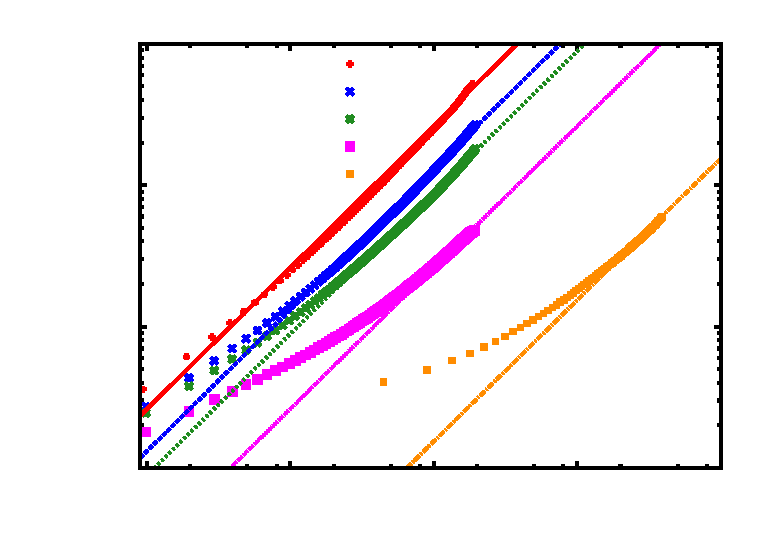
\includegraphics{./fit_msd}}%
    \gplfronttext
  \end{picture}%
\endgroup
\end{Large}}}%
	{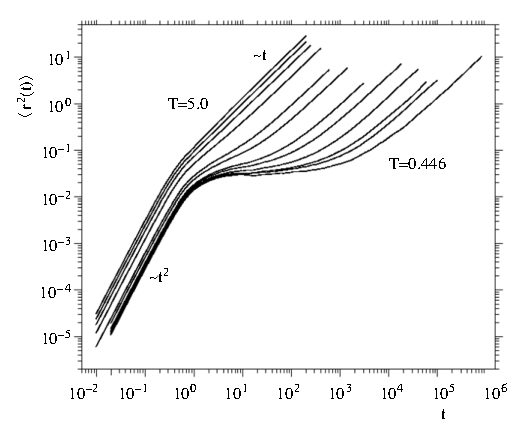
\includegraphics[width=\columnwidth, height=0.7\columnwidth]{msd_kob}}\\
	\alt<4>{\resizebox{\textwidth}{!}{\begin{Large}% GNUPLOT: LaTeX picture with Postscript
\begingroup
  \makeatletter
  \providecommand\color[2][]{%
    \GenericError{(gnuplot) \space\space\space\@spaces}{%
      Package color not loaded in conjunction with
      terminal option `colourtext'%
    }{See the gnuplot documentation for explanation.%
    }{Either use 'blacktext' in gnuplot or load the package
      color.sty in LaTeX.}%
    \renewcommand\color[2][]{}%
  }%
  \providecommand\includegraphics[2][]{%
    \GenericError{(gnuplot) \space\space\space\@spaces}{%
      Package graphicx or graphics not loaded%
    }{See the gnuplot documentation for explanation.%
    }{The gnuplot epslatex terminal needs graphicx.sty or graphics.sty.}%
    \renewcommand\includegraphics[2][]{}%
  }%
  \providecommand\rotatebox[2]{#2}%
  \@ifundefined{ifGPcolor}{%
    \newif\ifGPcolor
    \GPcolortrue
  }{}%
  \@ifundefined{ifGPblacktext}{%
    \newif\ifGPblacktext
    \GPblacktexttrue
  }{}%
  % define a \g@addto@macro without @ in the name:
  \let\gplgaddtomacro\g@addto@macro
  % define empty templates for all commands taking text:
  \gdef\gplbacktext{}%
  \gdef\gplfronttext{}%
  \makeatother
  \ifGPblacktext
    % no textcolor at all
    \def\colorrgb#1{}%
    \def\colorgray#1{}%
  \else
    % gray or color?
    \ifGPcolor
      \def\colorrgb#1{\color[rgb]{#1}}%
      \def\colorgray#1{\color[gray]{#1}}%
      \expandafter\def\csname LTw\endcsname{\color{white}}%
      \expandafter\def\csname LTb\endcsname{\color{black}}%
      \expandafter\def\csname LTa\endcsname{\color{black}}%
      \expandafter\def\csname LT0\endcsname{\color[rgb]{1,0,0}}%
      \expandafter\def\csname LT1\endcsname{\color[rgb]{0,1,0}}%
      \expandafter\def\csname LT2\endcsname{\color[rgb]{0,0,1}}%
      \expandafter\def\csname LT3\endcsname{\color[rgb]{1,0,1}}%
      \expandafter\def\csname LT4\endcsname{\color[rgb]{0,1,1}}%
      \expandafter\def\csname LT5\endcsname{\color[rgb]{1,1,0}}%
      \expandafter\def\csname LT6\endcsname{\color[rgb]{0,0,0}}%
      \expandafter\def\csname LT7\endcsname{\color[rgb]{1,0.3,0}}%
      \expandafter\def\csname LT8\endcsname{\color[rgb]{0.5,0.5,0.5}}%
    \else
      % gray
      \def\colorrgb#1{\color{black}}%
      \def\colorgray#1{\color[gray]{#1}}%
      \expandafter\def\csname LTw\endcsname{\color{white}}%
      \expandafter\def\csname LTb\endcsname{\color{black}}%
      \expandafter\def\csname LTa\endcsname{\color{black}}%
      \expandafter\def\csname LT0\endcsname{\color{black}}%
      \expandafter\def\csname LT1\endcsname{\color{black}}%
      \expandafter\def\csname LT2\endcsname{\color{black}}%
      \expandafter\def\csname LT3\endcsname{\color{black}}%
      \expandafter\def\csname LT4\endcsname{\color{black}}%
      \expandafter\def\csname LT5\endcsname{\color{black}}%
      \expandafter\def\csname LT6\endcsname{\color{black}}%
      \expandafter\def\csname LT7\endcsname{\color{black}}%
      \expandafter\def\csname LT8\endcsname{\color{black}}%
    \fi
  \fi
  \setlength{\unitlength}{0.0500bp}%
  \begin{picture}(7200.00,5040.00)%
    \gplgaddtomacro\gplbacktext{%
      \csname LTb\endcsname%
      \put(1056,704){\makebox(0,0)[r]{\strut{}$10^{0}$}}%
      \put(1056,1722){\makebox(0,0)[r]{\strut{}$10^{1}$}}%
      \put(1056,2740){\makebox(0,0)[r]{\strut{}$10^{2}$}}%
      \put(1056,3758){\makebox(0,0)[r]{\strut{}$10^{3}$}}%
      \put(1056,4776){\makebox(0,0)[r]{\strut{}$10^{4}$}}%
      \put(1967,484){\makebox(0,0){\strut{}$0.50$}}%
      \put(3165,484){\makebox(0,0){\strut{}$0.52$}}%
      \put(4363,484){\makebox(0,0){\strut{}$0.54$}}%
      \put(5562,484){\makebox(0,0){\strut{}$0.56$}}%
      \put(6760,484){\makebox(0,0){\strut{}$0.58$}}%
      \put(418,2740){\rotatebox{-270}{\makebox(0,0){\strut{}$t/\tau_B$}}}%
      \put(6979,2740){\rotatebox{-270}{\makebox(0,0){\strut{}}}}%
      \put(3974,154){\makebox(0,0){\strut{}$\phi$}}%
      \put(3974,4666){\makebox(0,0){\strut{}}}%
      \put(3974,4665){\makebox(0,0){\strut{}}}%
      \put(-132,110){\makebox(0,0)[l]{\strut{}}}%
    }%
    \gplgaddtomacro\gplfronttext{%
      \csname LTb\endcsname%
      \put(4620,4556){\makebox(0,0)[r]{\strut{}$\tau_\alpha$ experiments}}%
      \csname LTb\endcsname%
      \put(4620,4241){\makebox(0,0)[r]{\strut{}$\tau_\alpha$ simulations}}%
    }%
    \gplbacktext
    \put(0,0){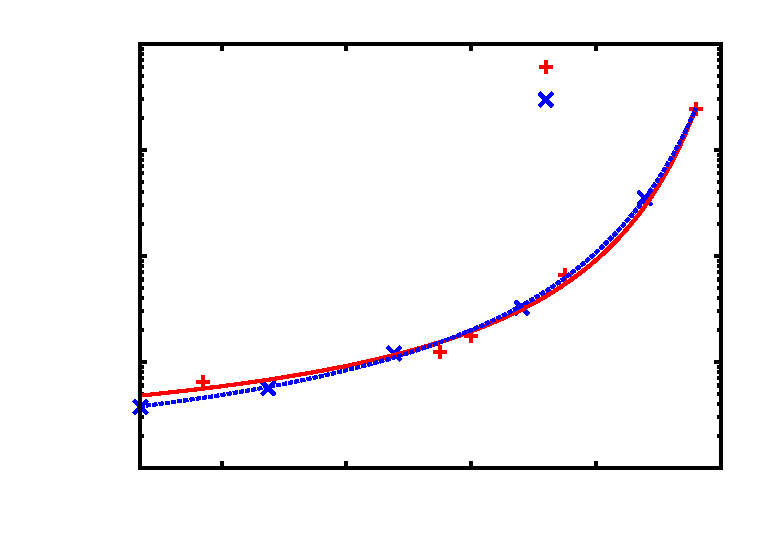
\includegraphics{fit_tau_alpha_vft}}%
    \gplfronttext
  \end{picture}%
\endgroup
\end{Large}}}%
		{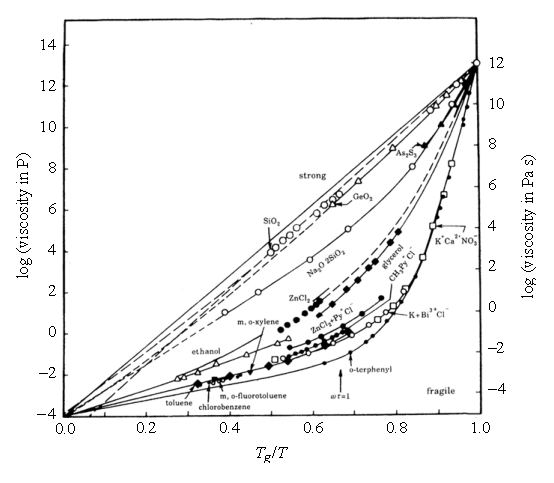
\includegraphics[width=\columnwidth, height=0.7\columnwidth]{angell}}
	\end{columns}
\end{frame}

\begin{frame}<all:1->{Dynamic heterogeneities}
	\begin{textblock*}{0.6\textwidth}(10mm,92mm)
		\simplephasediagram{%
		\node<all:1> at (0.497,0) [xp marker, fill=green!50!black] {};
		\node<all:2> at (0.535,0) [xp marker, fill=green!50!black] {};
		\node<all:3> at (0.576,0) [xp marker, fill=green!50!black] {};
		}
	\end{textblock*}
	\begin{columns}[T]
	\column{0.6\textwidth}
	\only<all:1>{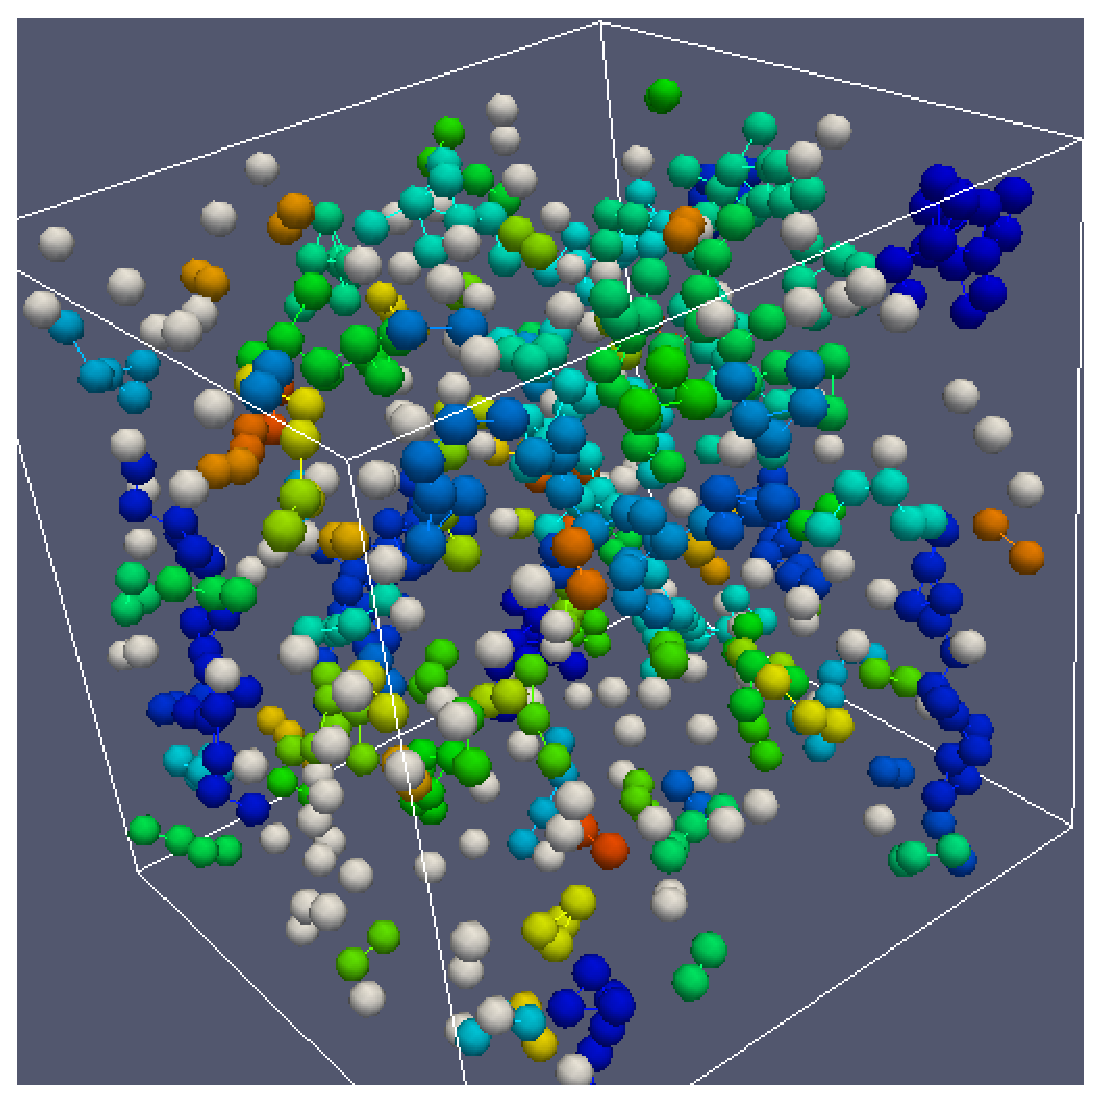
\includegraphics[width=\columnwidth]{dh_3954}
	\[ \phi=0.497 \]}%
	\only<all:2>{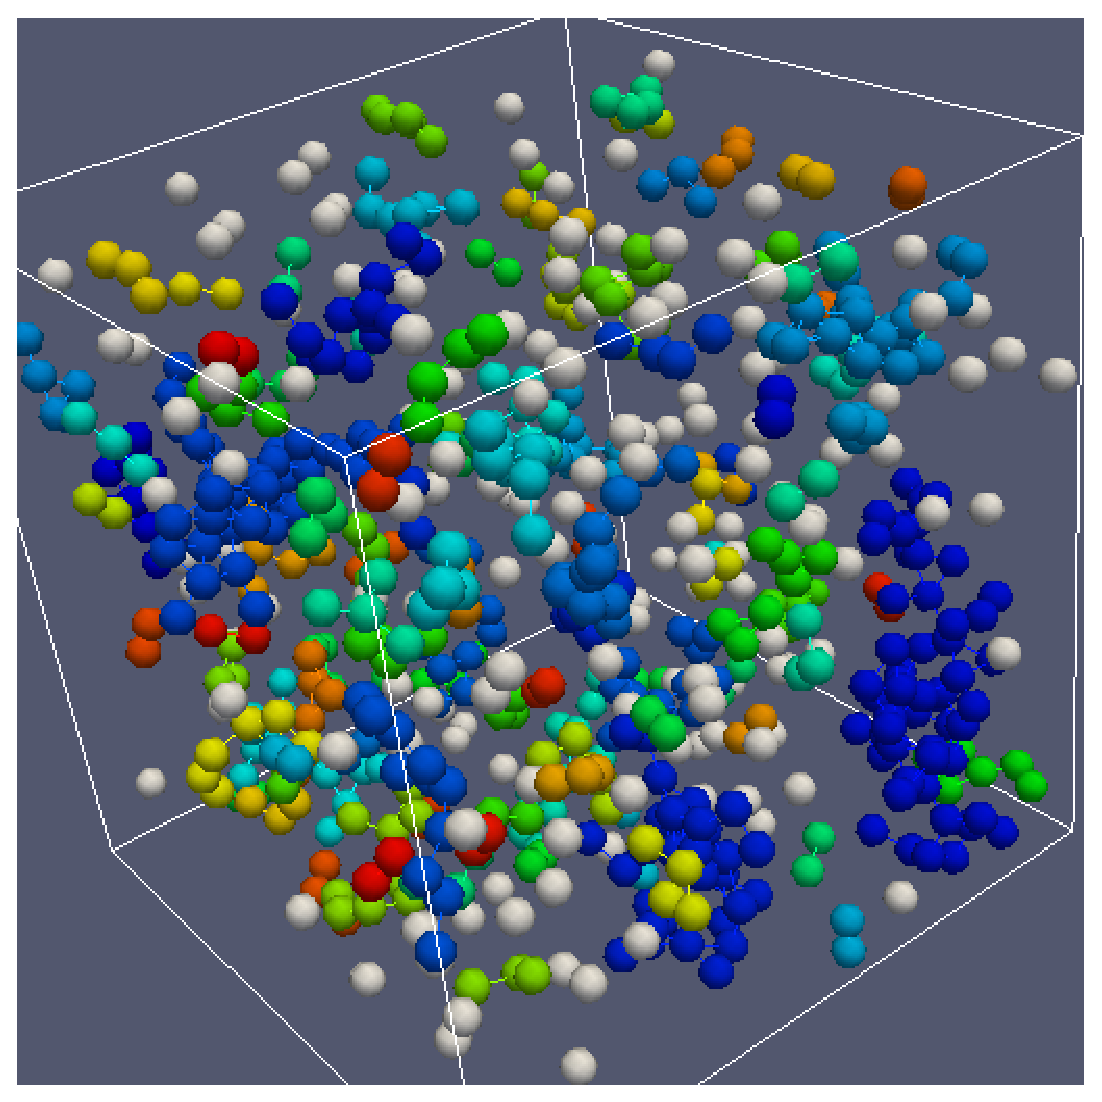
\includegraphics[width=\columnwidth]{dh_4582}
	\[ \phi=0.535 \]}%
	\only<all:3>{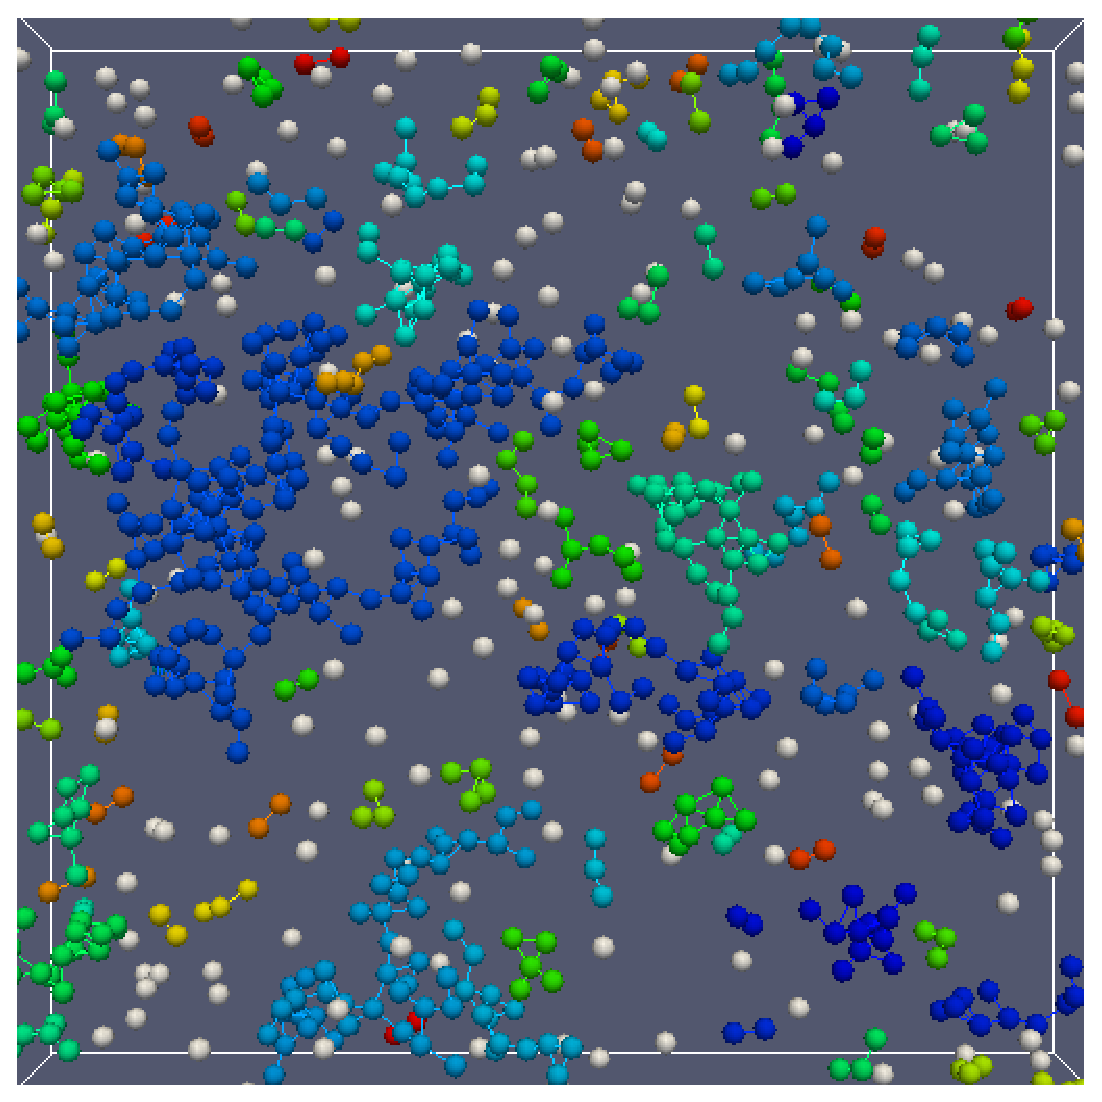
\includegraphics[width=\columnwidth]{dh_go1}
	\[ \phi=0.576 \]}%
	\column{0.4\textwidth}
	\begin{block}{$10\%$ fastest particles}
	\begin{itemize}
		\item isolated \tikz\shade[ball color=white] (0,0) circle (0.5em);
		\item connected \begin{tikzpicture}
			\shade[ball color=blue] (0,0) circle (0.5em);
			\shade[ball color=green] +(1em,0) circle (0.5em);
			\shade[ball color=yellow] +(2em,0) circle (0.5em);
			\shade[ball color=red] +(3em,0) circle (0.5em);
			\end{tikzpicture}
	\end{itemize}
	\end{block}
	\begin{itemize}
		\item Rearrangements group in space
		\item Growing characteristic size
	\end{itemize}
	\end{columns}
\end{frame}

\begin{frame}{Dynamic correlation length}
	\begin{textblock*}{0.6\textwidth}(10mm,92mm)
		\simplephasediagram{}
	\end{textblock*}
	Spatial correlation of the fluctuations of the displacement
	\begin{columns}
	\column{0.6\textwidth}
	\[ \mathcal{G}_u(r,t) \equiv \frac{
		\left\langle \sum_{i,j}{\delta u_i(t) \delta u_j(t) \delta(r_{ij} -r)} \right\rangle 
	}{
		\left\langle \sum_{i,j}{\delta(r_{ij} -r)} \right\rangle
	}\]
	\column{0.4\textwidth}
	\begin{align*}
		u_i(t) \equiv & \|\vec{r}_i(t)-\vec{r}_i(0)\|\\
		\delta u_i \equiv& u_i- \langle u_i \rangle
	\end{align*}
	\end{columns}
	\begin{columns}
	\column{0.6\textwidth}
	\resizebox{\columnwidth}{!}{\begin{Large}% GNUPLOT: LaTeX picture with Postscript
\begingroup
  \makeatletter
  \providecommand\color[2][]{%
    \GenericError{(gnuplot) \space\space\space\@spaces}{%
      Package color not loaded in conjunction with
      terminal option `colourtext'%
    }{See the gnuplot documentation for explanation.%
    }{Either use 'blacktext' in gnuplot or load the package
      color.sty in LaTeX.}%
    \renewcommand\color[2][]{}%
  }%
  \providecommand\includegraphics[2][]{%
    \GenericError{(gnuplot) \space\space\space\@spaces}{%
      Package graphicx or graphics not loaded%
    }{See the gnuplot documentation for explanation.%
    }{The gnuplot epslatex terminal needs graphicx.sty or graphics.sty.}%
    \renewcommand\includegraphics[2][]{}%
  }%
  \providecommand\rotatebox[2]{#2}%
  \@ifundefined{ifGPcolor}{%
    \newif\ifGPcolor
    \GPcolortrue
  }{}%
  \@ifundefined{ifGPblacktext}{%
    \newif\ifGPblacktext
    \GPblacktexttrue
  }{}%
  % define a \g@addto@macro without @ in the name:
  \let\gplgaddtomacro\g@addto@macro
  % define empty templates for all commands taking text:
  \gdef\gplbacktext{}%
  \gdef\gplfronttext{}%
  \makeatother
  \ifGPblacktext
    % no textcolor at all
    \def\colorrgb#1{}%
    \def\colorgray#1{}%
  \else
    % gray or color?
    \ifGPcolor
      \def\colorrgb#1{\color[rgb]{#1}}%
      \def\colorgray#1{\color[gray]{#1}}%
      \expandafter\def\csname LTw\endcsname{\color{white}}%
      \expandafter\def\csname LTb\endcsname{\color{black}}%
      \expandafter\def\csname LTa\endcsname{\color{black}}%
      \expandafter\def\csname LT0\endcsname{\color[rgb]{1,0,0}}%
      \expandafter\def\csname LT1\endcsname{\color[rgb]{0,1,0}}%
      \expandafter\def\csname LT2\endcsname{\color[rgb]{0,0,1}}%
      \expandafter\def\csname LT3\endcsname{\color[rgb]{1,0,1}}%
      \expandafter\def\csname LT4\endcsname{\color[rgb]{0,1,1}}%
      \expandafter\def\csname LT5\endcsname{\color[rgb]{1,1,0}}%
      \expandafter\def\csname LT6\endcsname{\color[rgb]{0,0,0}}%
      \expandafter\def\csname LT7\endcsname{\color[rgb]{1,0.3,0}}%
      \expandafter\def\csname LT8\endcsname{\color[rgb]{0.5,0.5,0.5}}%
    \else
      % gray
      \def\colorrgb#1{\color{black}}%
      \def\colorgray#1{\color[gray]{#1}}%
      \expandafter\def\csname LTw\endcsname{\color{white}}%
      \expandafter\def\csname LTb\endcsname{\color{black}}%
      \expandafter\def\csname LTa\endcsname{\color{black}}%
      \expandafter\def\csname LT0\endcsname{\color{black}}%
      \expandafter\def\csname LT1\endcsname{\color{black}}%
      \expandafter\def\csname LT2\endcsname{\color{black}}%
      \expandafter\def\csname LT3\endcsname{\color{black}}%
      \expandafter\def\csname LT4\endcsname{\color{black}}%
      \expandafter\def\csname LT5\endcsname{\color{black}}%
      \expandafter\def\csname LT6\endcsname{\color{black}}%
      \expandafter\def\csname LT7\endcsname{\color{black}}%
      \expandafter\def\csname LT8\endcsname{\color{black}}%
    \fi
  \fi
  \setlength{\unitlength}{0.0500bp}%
  \begin{picture}(7200.00,5040.00)%
    \gplgaddtomacro\gplbacktext{%
      \csname LTb\endcsname%
      \put(1056,704){\makebox(0,0)[r]{\strut{}$10^{-4}$}}%
      \put(1056,1938){\makebox(0,0)[r]{\strut{}$10^{-3}$}}%
      \put(1056,3171){\makebox(0,0)[r]{\strut{}$10^{-2}$}}%
      \put(1056,4405){\makebox(0,0)[r]{\strut{}$10^{-1}$}}%
      \put(1368,484){\makebox(0,0){\strut{}$2$}}%
      \put(2266,484){\makebox(0,0){\strut{}$3$}}%
      \put(3165,484){\makebox(0,0){\strut{}$4$}}%
      \put(4064,484){\makebox(0,0){\strut{}$5$}}%
      \put(4963,484){\makebox(0,0){\strut{}$6$}}%
      \put(5861,484){\makebox(0,0){\strut{}$7$}}%
      \put(6760,484){\makebox(0,0){\strut{}$8$}}%
      \put(286,2740){\rotatebox{-270}{\makebox(0,0){\strut{}$\mathcal{G}_u(r,t^{dh})/\Delta r^2(t^{dh})$}}}%
      \put(6979,2740){\rotatebox{-270}{\makebox(0,0){\strut{}}}}%
      \put(3974,154){\makebox(0,0){\strut{}$r/\sigma$}}%
      \put(3974,4666){\makebox(0,0){\strut{}}}%
      \put(3974,4665){\makebox(0,0){\strut{}}}%
      \put(-264,110){\makebox(0,0)[l]{\strut{}}}%
    }%
    \gplgaddtomacro\gplfronttext{%
      \csname LTb\endcsname%
      \put(2904,932){\makebox(0,0)[r]{\strut{}$\phi=0.497$}}%
      \csname LTb\endcsname%
      \put(2904,1262){\makebox(0,0)[r]{\strut{}$\phi=0.555$}}%
      \csname LTb\endcsname%
      \put(2904,1592){\makebox(0,0)[r]{\strut{}$\phi=0.576$}}%
    }%
    \gplbacktext
    \put(0,0){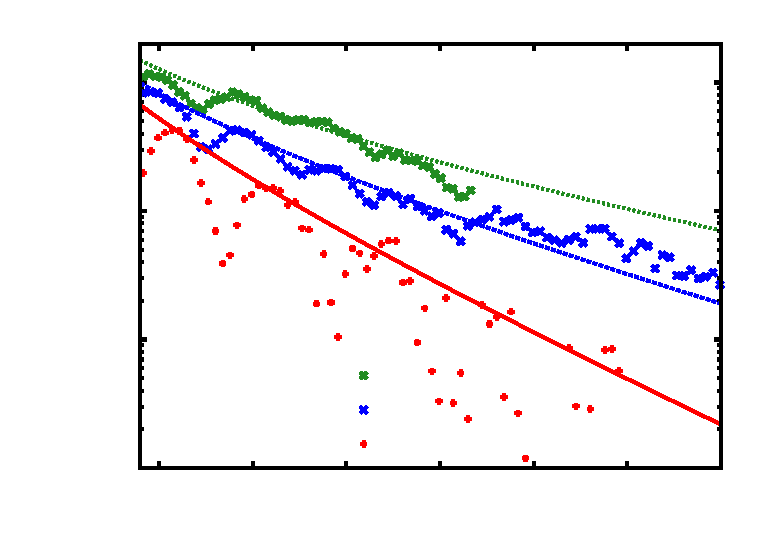
\includegraphics{fit_gu}}%
    \gplfronttext
  \end{picture}%
\endgroup
\end{Large}}
	\column{0.4\textwidth}
	Ornstein-Zernike fit
	\[ \mathcal{G}_u(r,t^{dh}) \propto r^{-1}\exp( -\frac{r}{\xi_u} )\]
	$\xi_u$ grows when approaching the glass transition
	\end{columns}
\end{frame}

\begin{frame}{Our system}
	\begin{itemize}
		\item Exhibits the phenomenology of the glass transition
		\item Is a valid model system
		\item Allows access to the scale of its elementary particles
	\end{itemize}
	\bigskip $\Rightarrow$ We can investigate both the dynamics and the structure at the particle level
\end{frame}

\section[Structure]{Structural heterogeneities}
\subsection{Identification}

\begin{frame}{Usual way to identify structures: Diffraction}
	\begin{columns}
	\column{0.5\textwidth}
	\def\svgwidth{\columnwidth}\input{xray.pdf_tex}
	\begin{itemize}
		\item Average over illuminated area
		\item Long ranged positional order
		\item Coherent orientation
	\end{itemize}
	\column{0.5\textwidth}
	\centering Quasi-crystal\\
	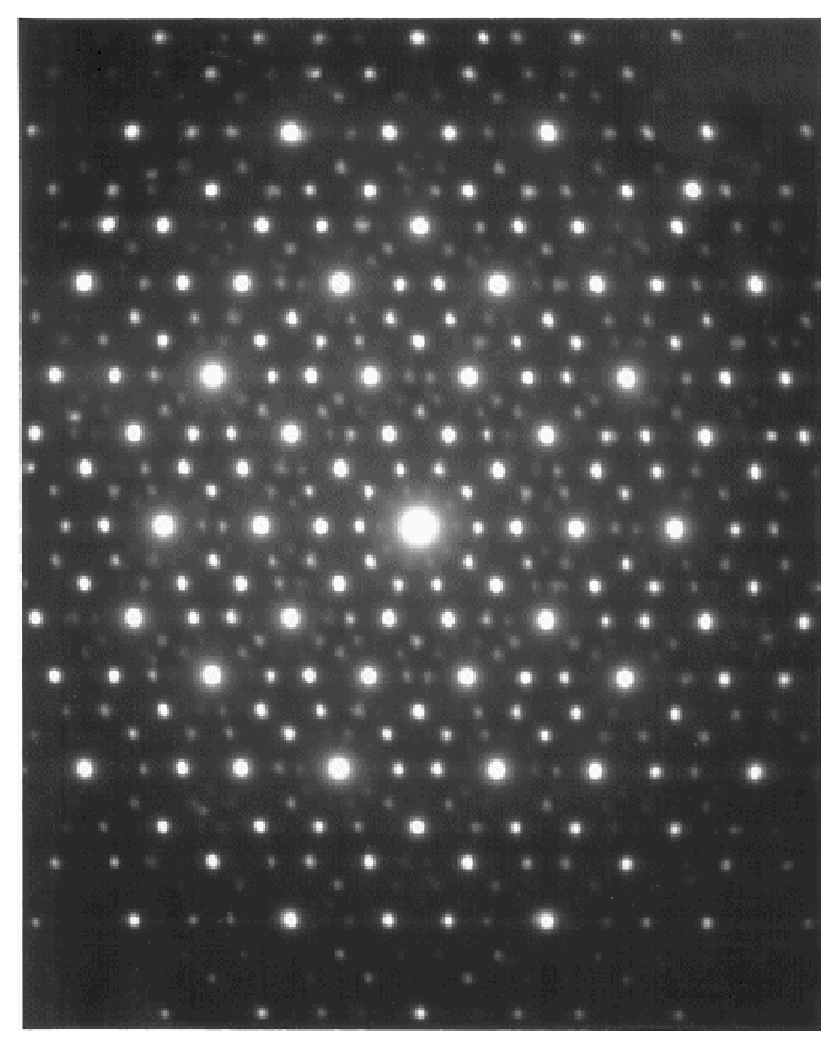
\includegraphics[width=\columnwidth]{diffraction_quasiX}
	\end{columns}
\end{frame}

\begin{frame}{Local symmetry}
	\begin{center}
	\begin{tikzpicture}[scale=0.3]
		\tikzset{particle/.style={circle, ball color=blue!50!white, inner sep=0, minimum size=2em}}
		\tikzset{ar/.style={->, draw=red!80!black, thick}}
		\node[particle] at (14.356, 47.436) (a) {};
		\node[particle] at (17.000, 52.387) (b) {};
		\node[particle] at (20.000, 48.000) (c) {};
		\node[particle] at (17.178, 44.149) (d) {};
		\node[particle] at (22.258, 51.951) (e) {};
		\node[particle] at (22.822, 44.049) (f) {};
		\node[particle] at (23.387, 56.467) (g) {};
		\node[particle] at (27.902, 58.160) (g1) {};
		\node[particle] at (26.773, 53.080) (h) {};
		\node[particle] at (25.644, 48.000) (i) {};
		\node[particle] at (31.300, 54.773) (j) {};
		\node[particle] at (30.724, 49.693) (k) {};
		\node[particle] at (36.000, 57.596) (k1) {};
		\node[particle] at (35.804, 53.016) (l) {};
		\node[particle] at (34.676, 47.436) (m) {};
		\node[particle] at (40.320, 54.209) (n) {};
		\node[particle] at (39.191, 49.129) (o) {};
		\path[ar] (d) edge (c);
		\path[ar] (c) edge (e);
		\path[ar] (i) edge (h);
		\path[ar] (k) edge (j);
		\path[ar] (l) edge (k1);
		\draw[green!50!black] (a) -- (c) -- (b);
		\path[green!50!black,<->] (a) edge [bend left] (b);
		\draw[green!50!black] (n) -- (l) -- (o);
		\path[green!50!black,<->] (n) edge [bend left] (o);
	\end{tikzpicture}
	\begin{itemize}
		\item The orientation changes $\Rightarrow$ No positional order
		\item The local angles stay the same $\Rightarrow$ Bond orientational order
	\end{itemize}
	\end{center}
\end{frame}

\begin{frame}{Local structures}
	\begin{center}\begin{tabular}{ccc}
	FCC & HCP & Icosahedron \\ 
	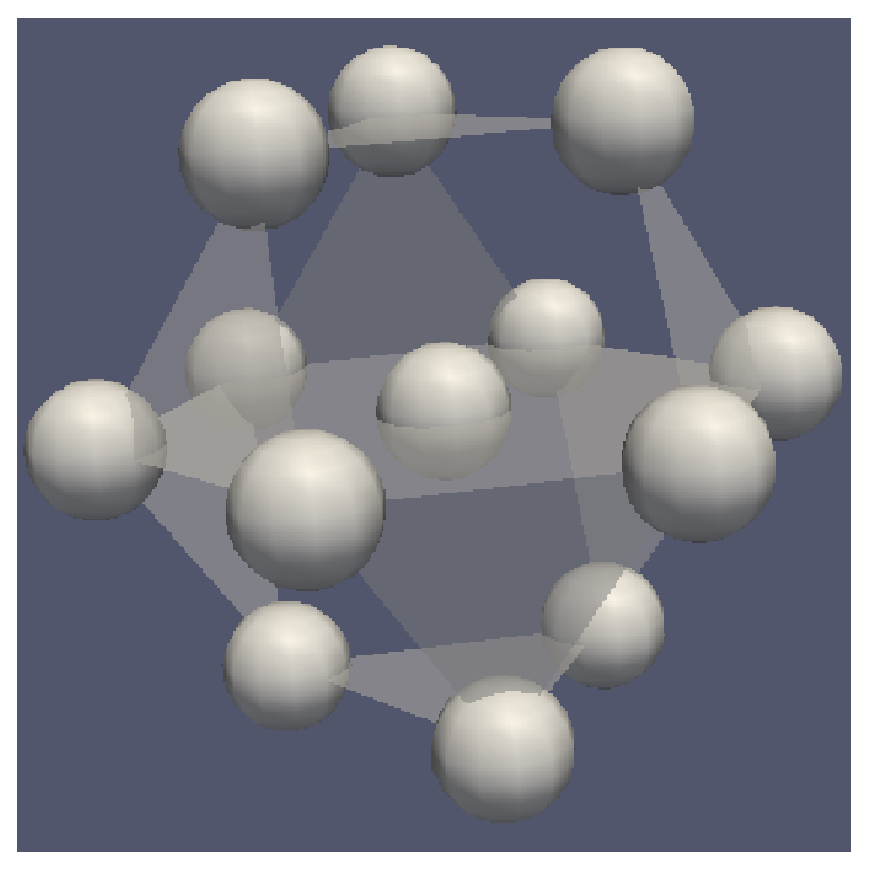
\includegraphics[width=0.27\textwidth]{fcc_13} & 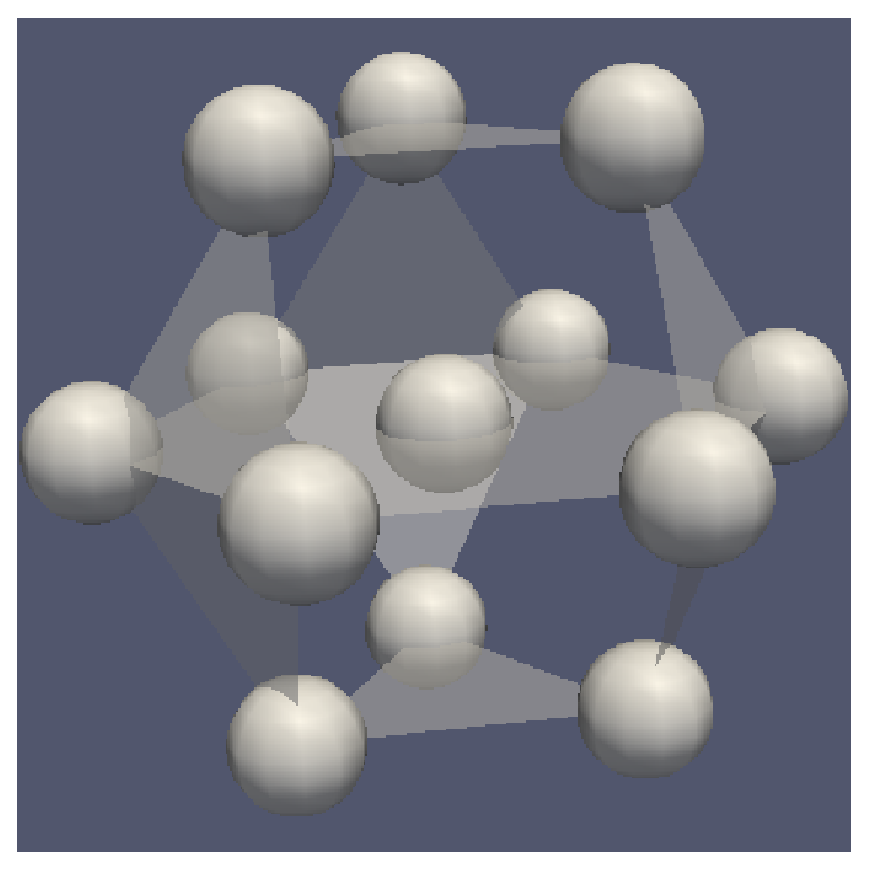
\includegraphics[width=0.27\textwidth]{hcp_13} & 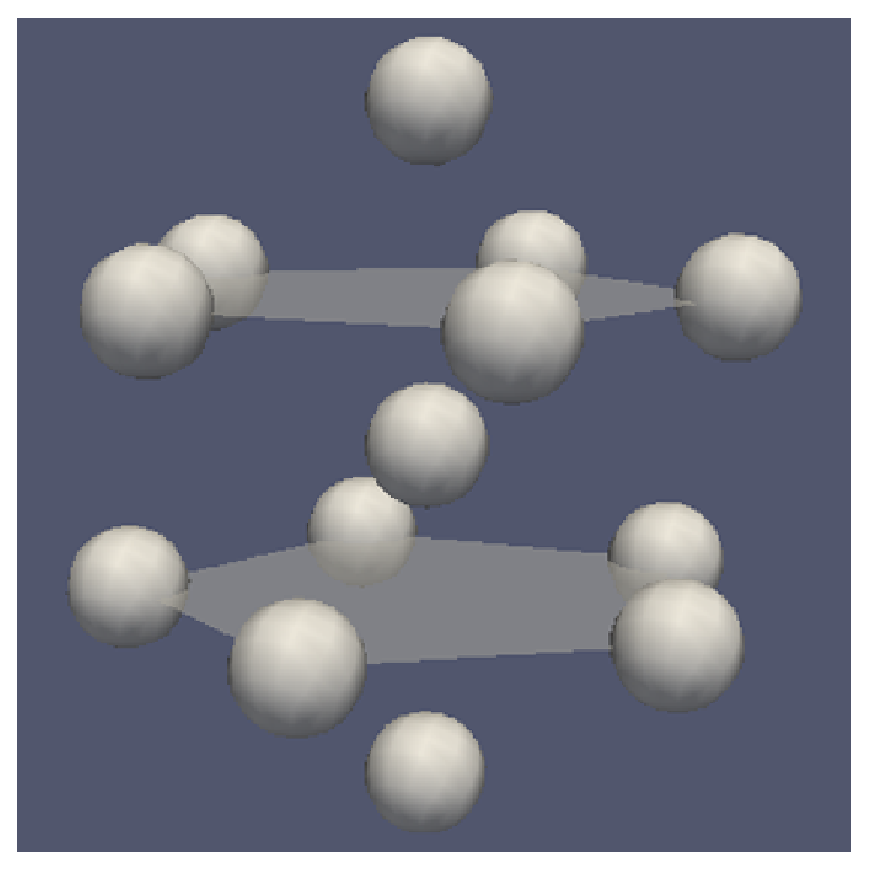
\includegraphics[width=0.27\textwidth]{ico_13}
	\end{tabular}
	\only<all:1>{\begin{tabular}{ccc}
	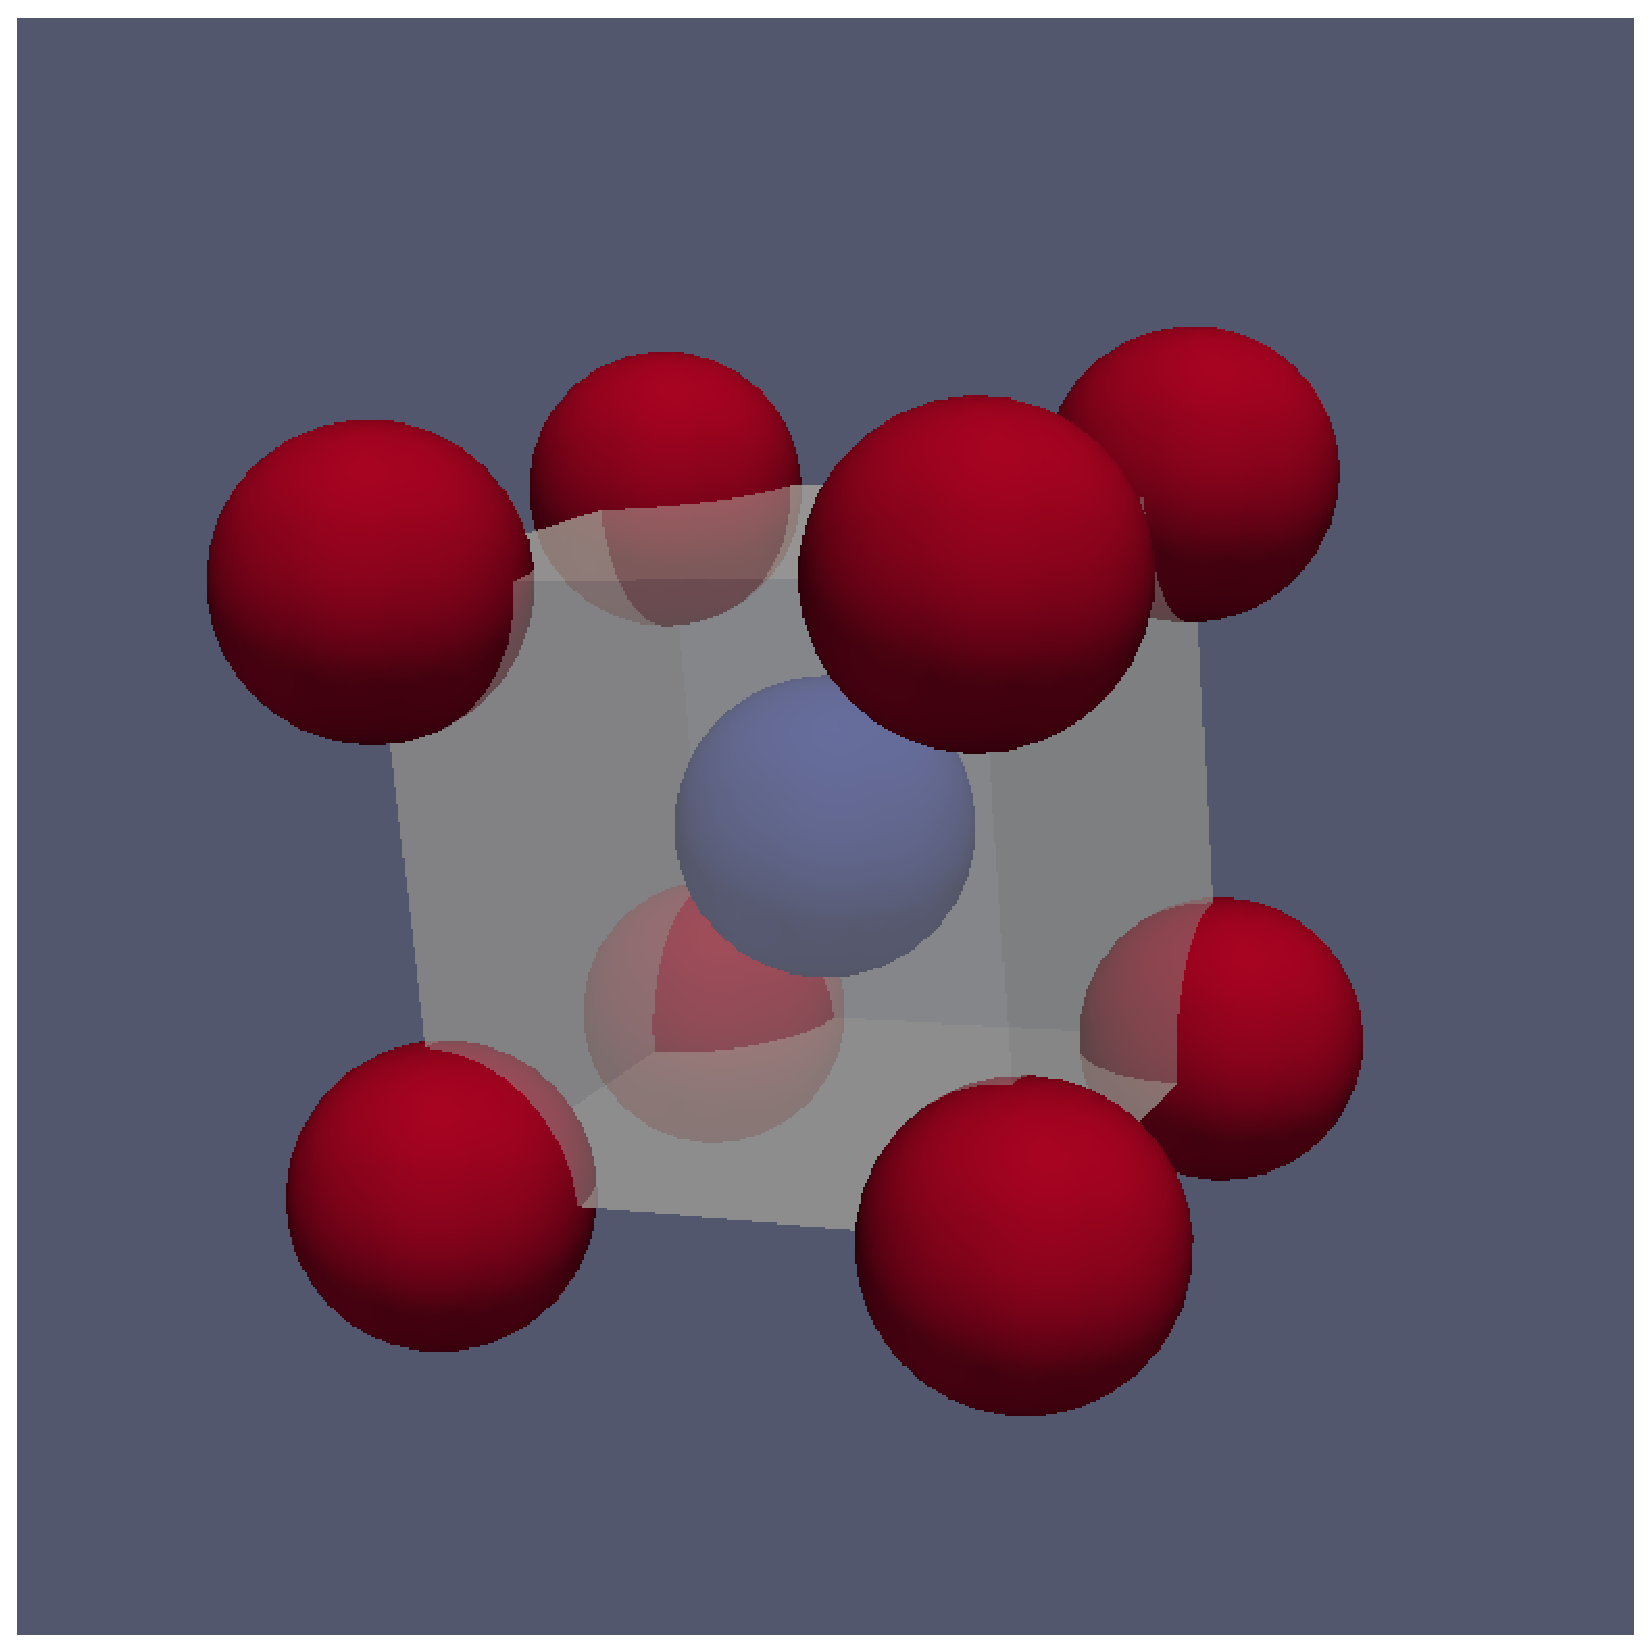
\includegraphics[width=0.27\textwidth]{bcc_9} & 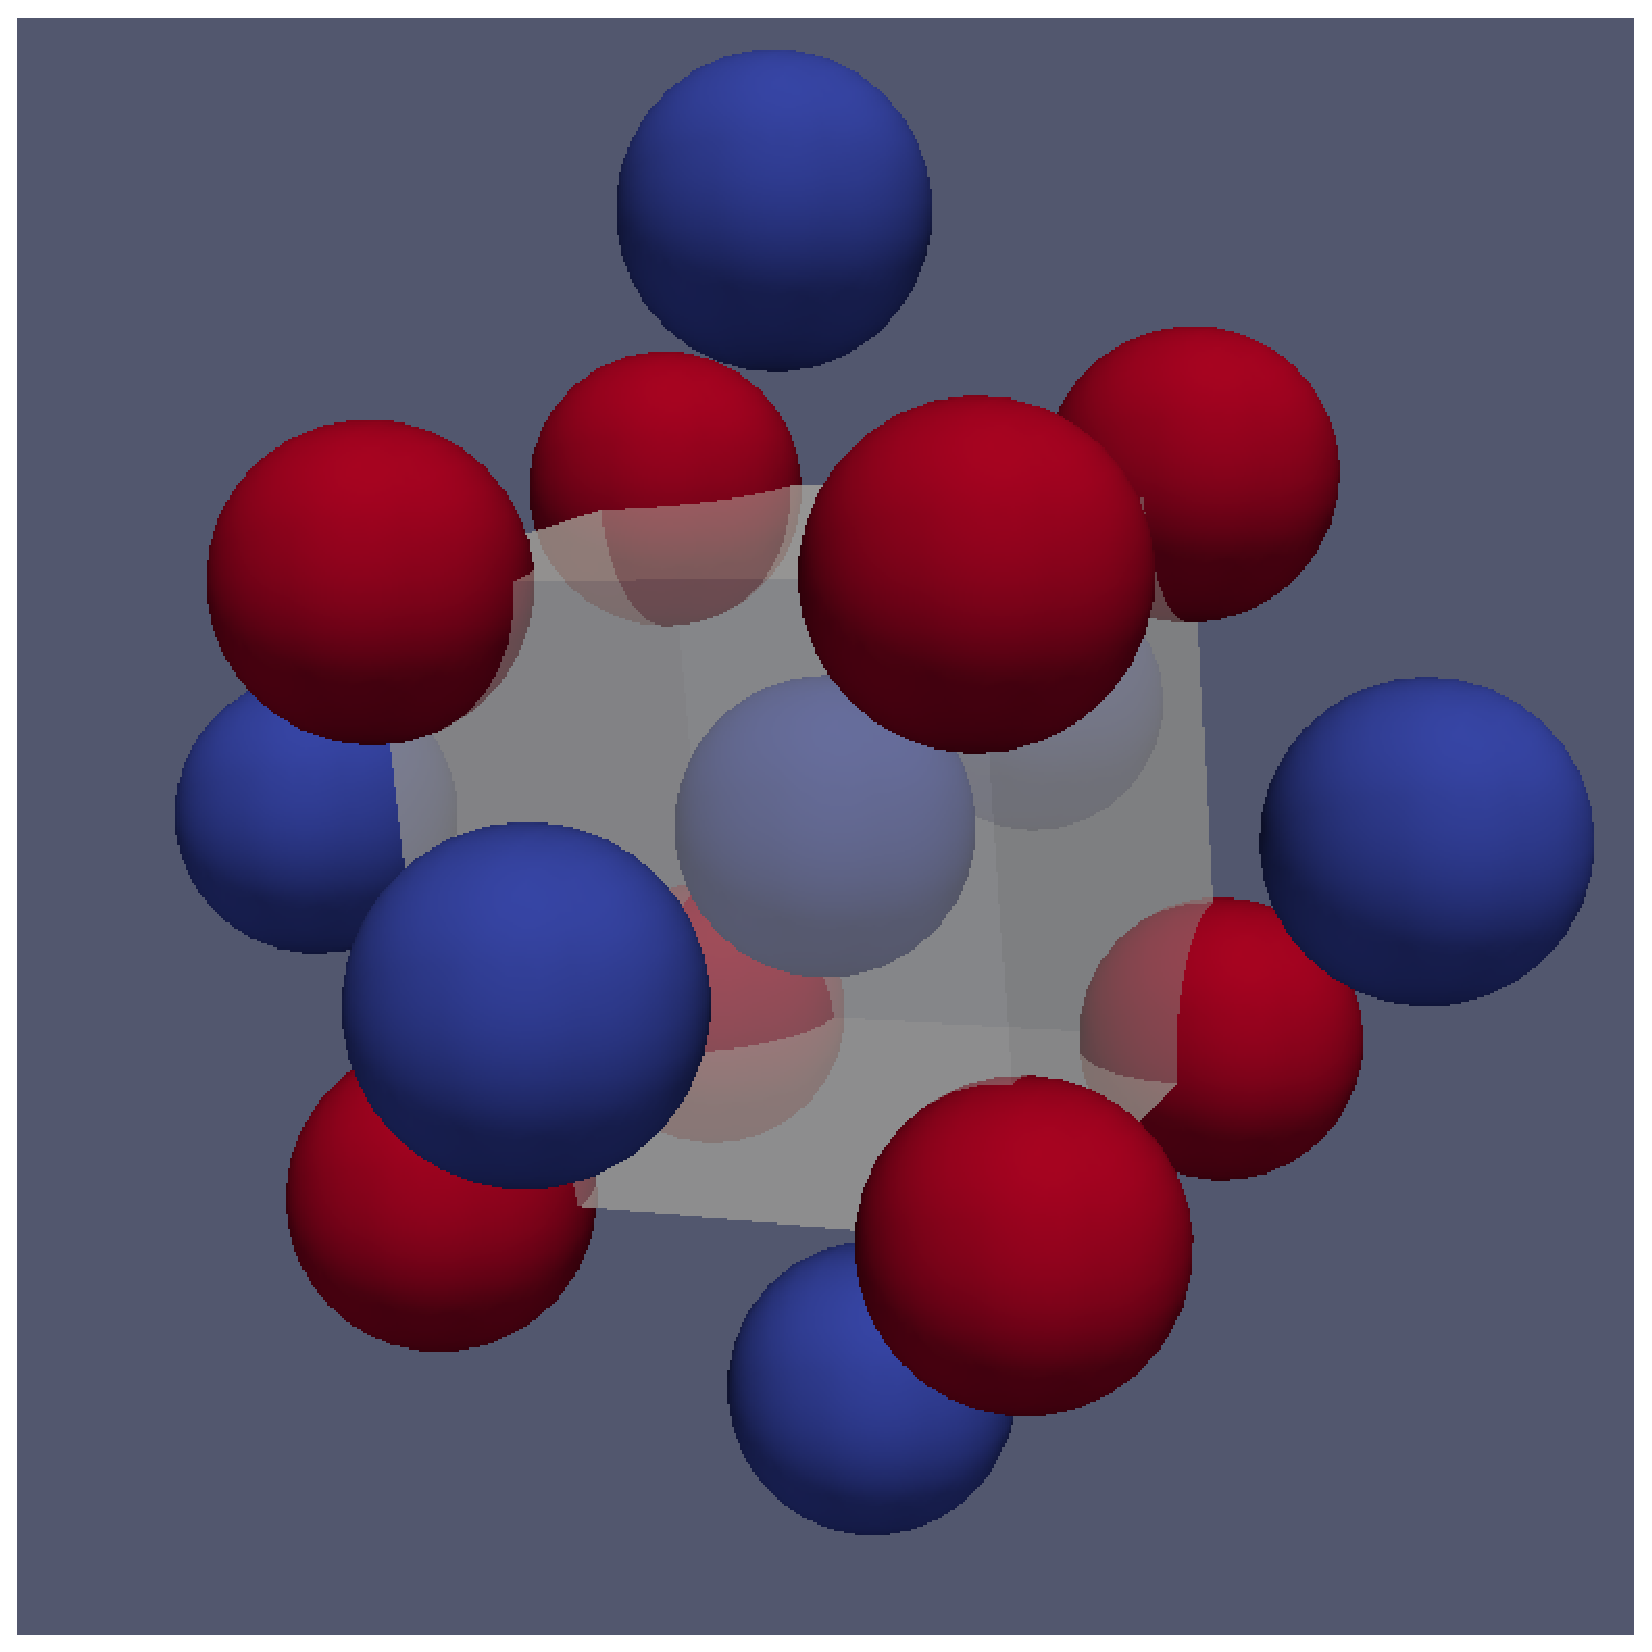
\includegraphics[width=0.27\textwidth]{bcc_15} & 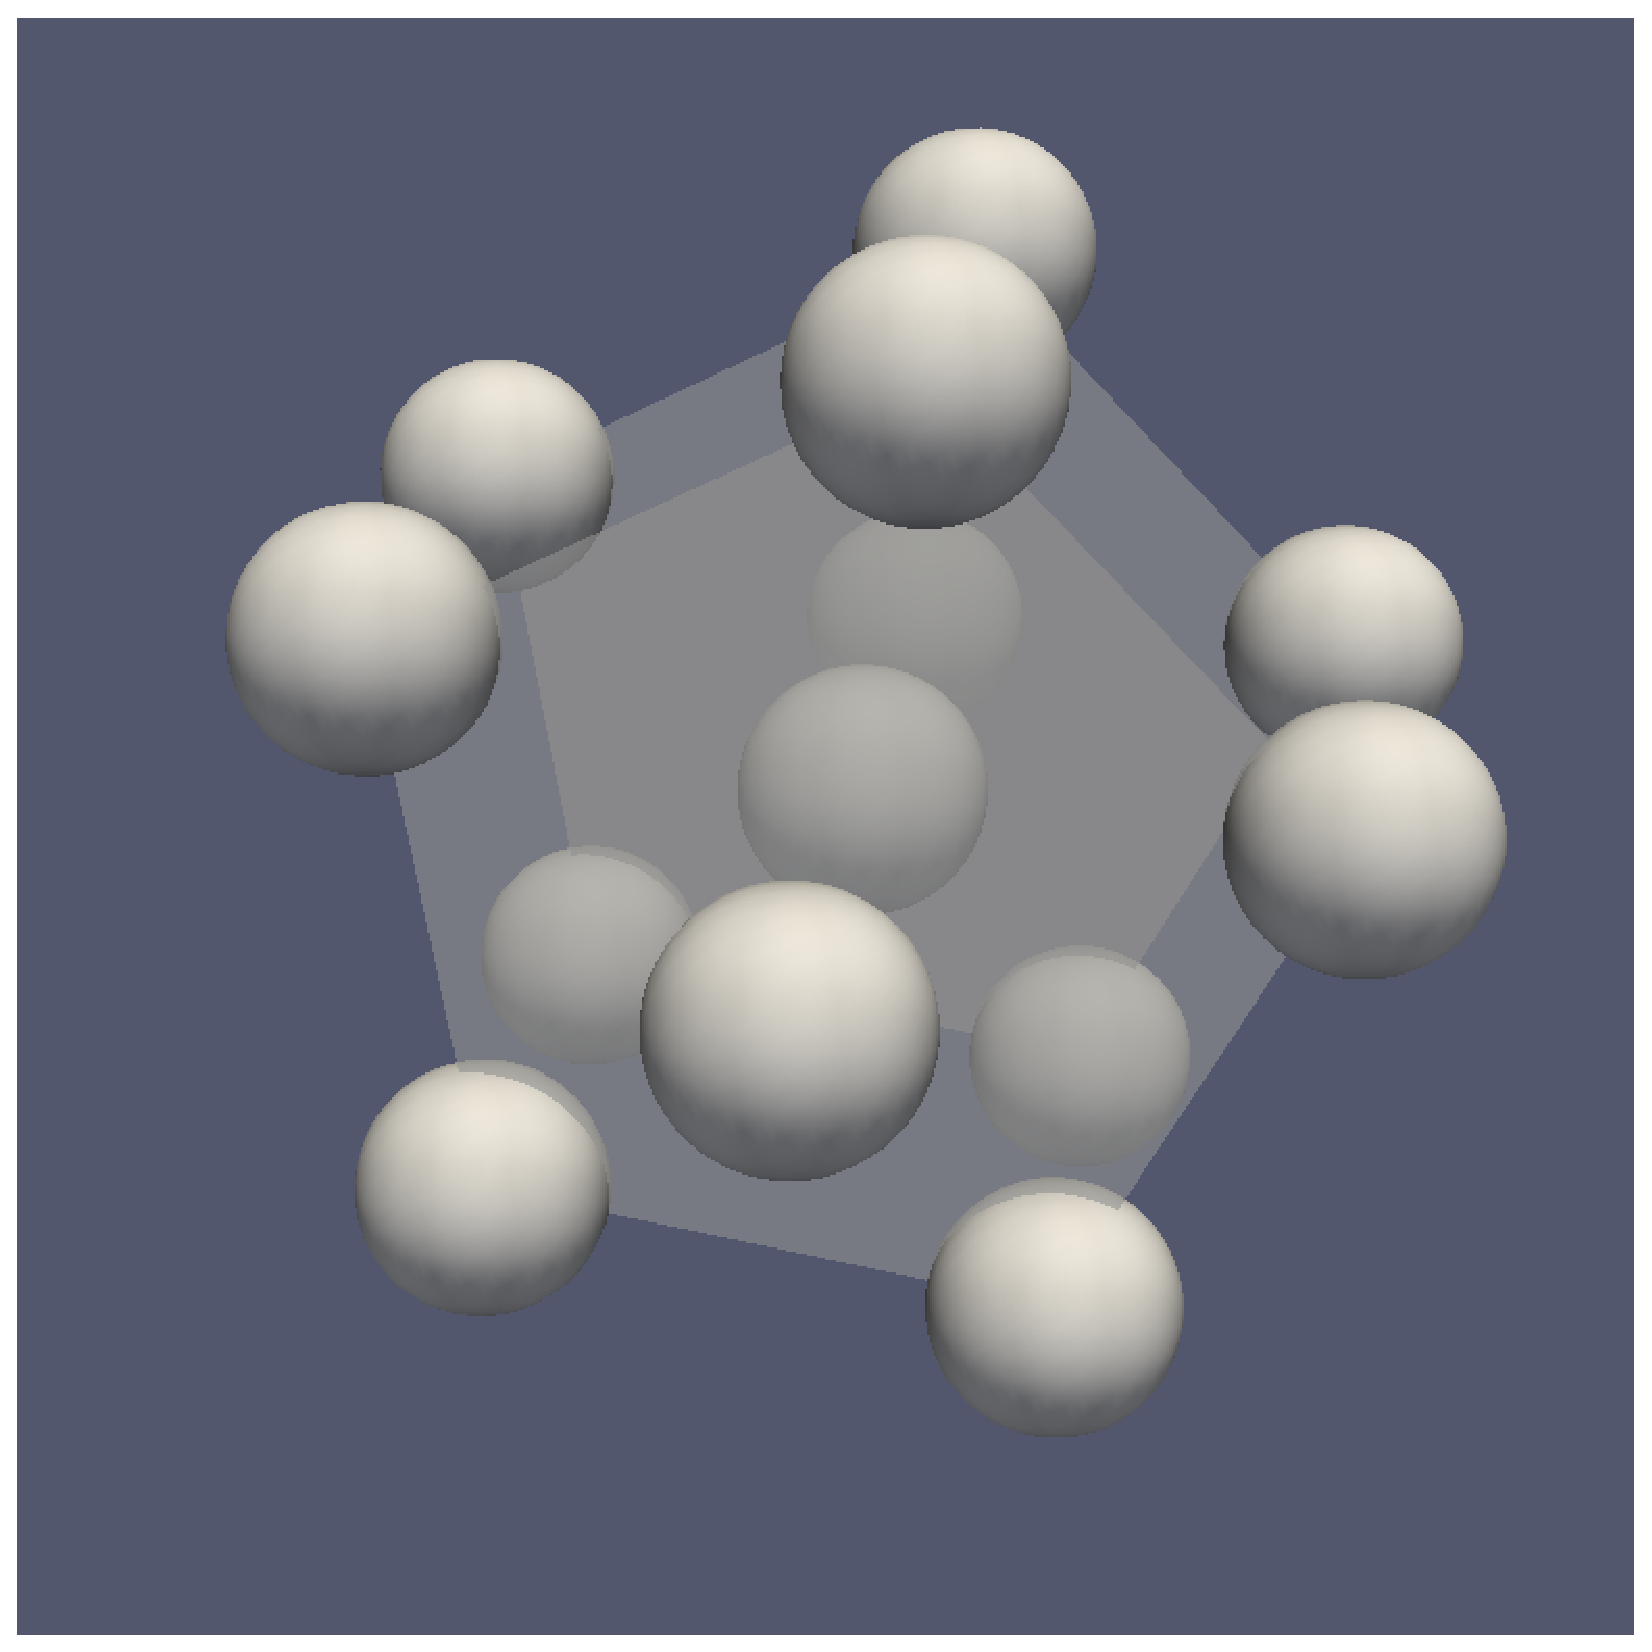
\includegraphics[width=0.27\textwidth]{dodec_13} \\ 
	BCC 9 & BCC 15 & Dodecadehron \\ 
	\end{tabular}}%
	\end{center}
	\only<all:2>{%
	\begin{itemize}
		\item The best ways to pack particles
		\item In hard spheres
		\begin{itemize}
			\item no potential energy
			\item ordering maximizes local vibrations
			\item vibrational entropy $\Leftrightarrow$ configurational entropy
			\item packing drives ordering
		\end{itemize}
	\end{itemize}
	
	\bigskip}%
\end{frame}

\begin{frame}[label=local_sym_sh]{Local symmetries and spherical harmonics}
	\begin{columns}
	\centering
	\column{0.25\textwidth}
	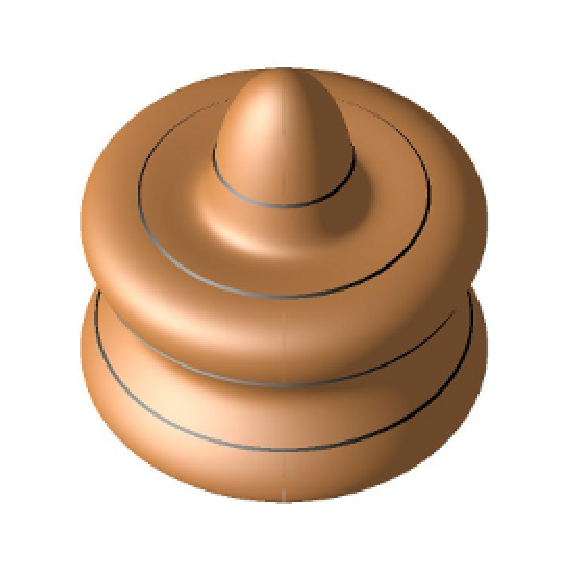
\includegraphics[width=\columnwidth]{sh6-0}\\
	\centering{$\ell=6, m=0$}
	\column{0.05\textwidth}
	$+$
	\column{0.25\textwidth}
	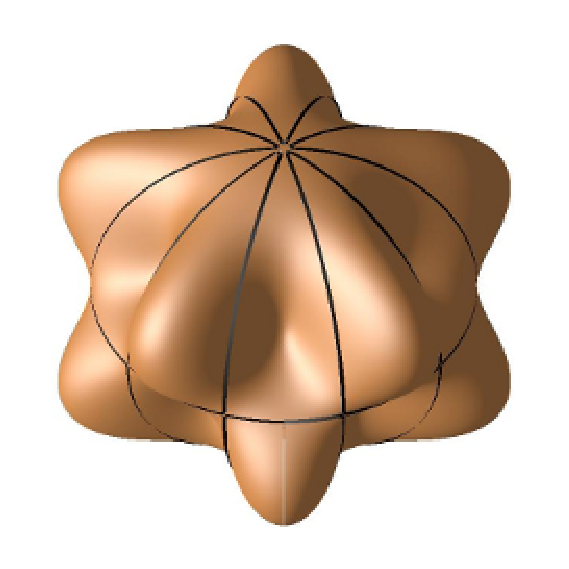
\includegraphics[width=\columnwidth]{sh6-5}\\
	\centering{$\ell=6, m=5$}
	\column{0.05\textwidth}
	$=$
	\column{0.3\textwidth}
	\centering{Icosahedron}\\
	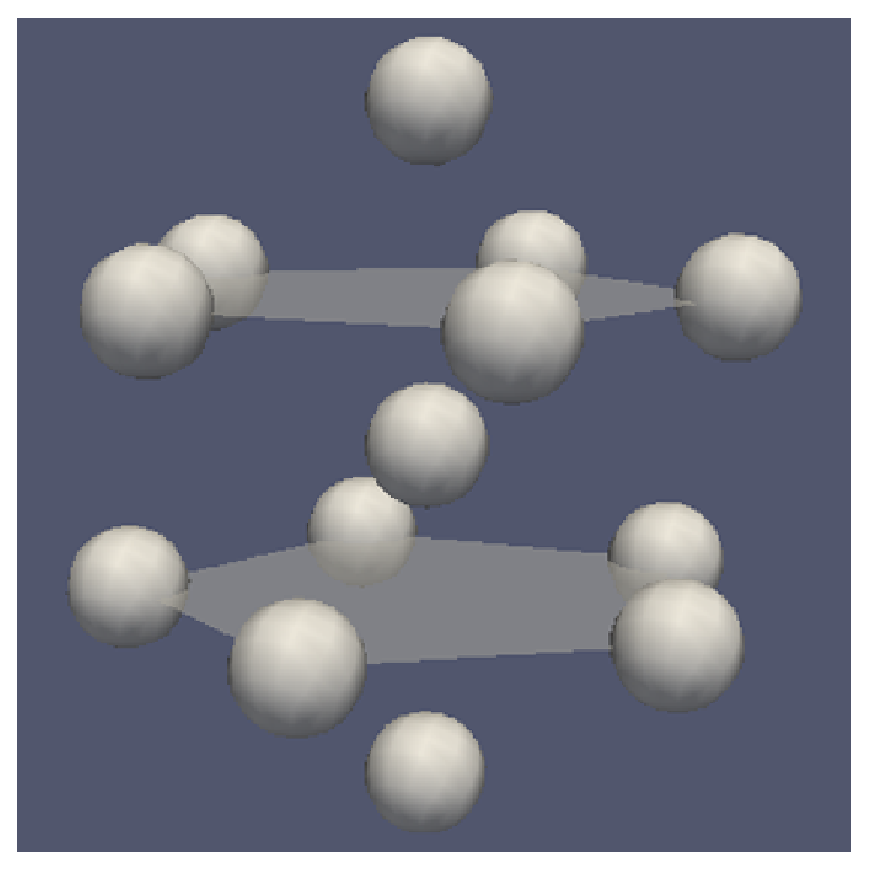
\includegraphics[width=\columnwidth]{ico_13}
	\end{columns}
	
	\begin{columns}
	\centering
	\column{0.25\textwidth}
	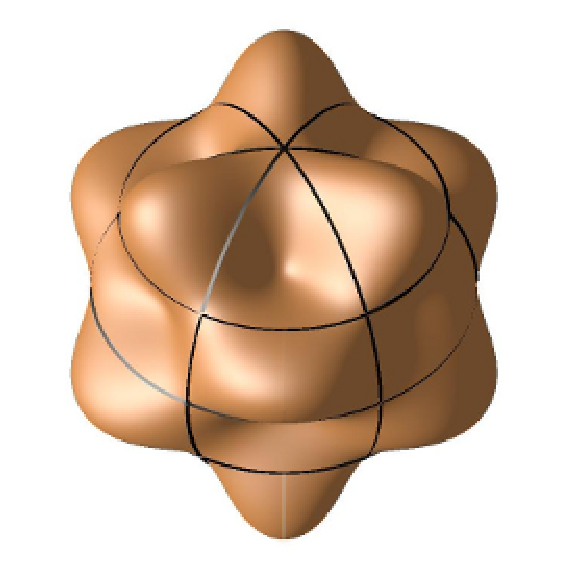
\includegraphics[width=\columnwidth]{sh6-3}\\
	\centering{$\ell=6, m=3$}
	\column{0.05\textwidth}
	$+$
	\column{0.25\textwidth}
	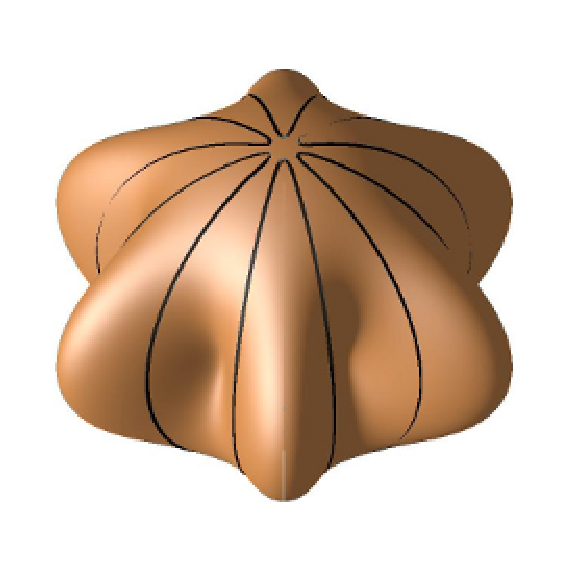
\includegraphics[width=\columnwidth]{sh6-6}\\
	\centering{$\ell=6, m=6$}
	\column{0.05\textwidth}
	$=$
	\column{0.3\textwidth}
	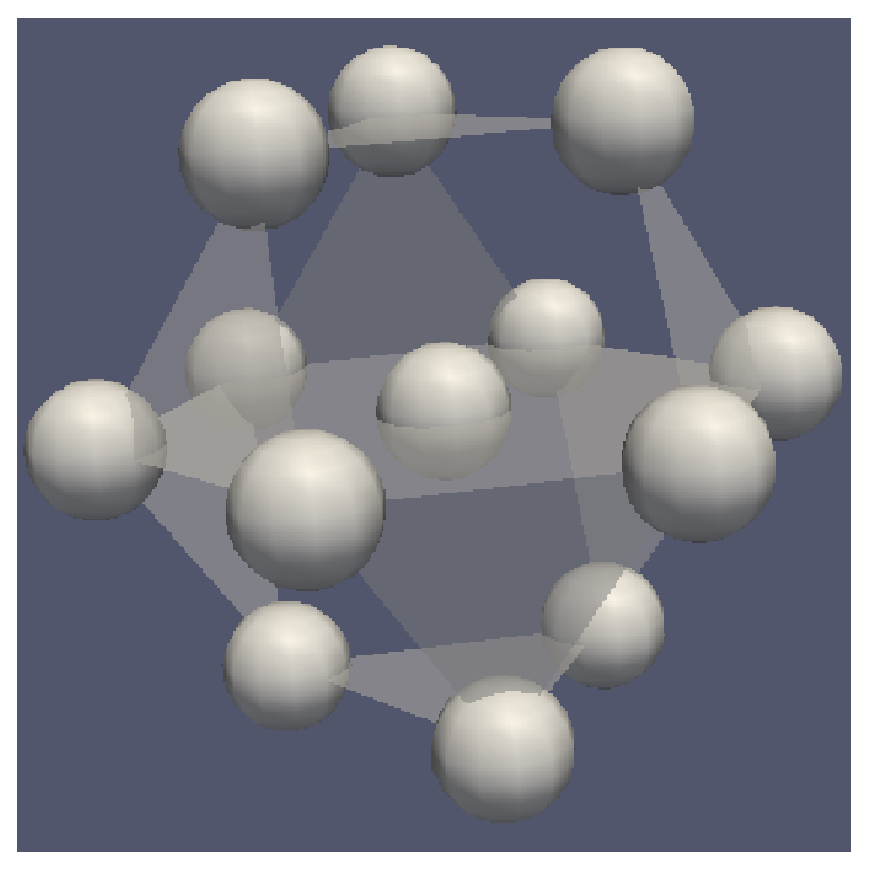
\includegraphics[width=\columnwidth]{fcc_13}\\
	\centering{FCC}
	\end{columns}
\end{frame}

\begin{frame}{Bond orientational order}
	\begin{columns}
	\column{0.5\textwidth}
	\includegraphics[width=\columnwidth]{lechner_Q4Q6}
	\column{0.5\textwidth}
	\begin{itemize}
		\item $Q_\ell$ is the strength of the $\ell$-fold symmetry
		\item Very good at telling apart
			\begin{itemize}
				\item aperiodic structures
				\item locally periodic
			\end{itemize}
		\item Differentiate between crystal structures
	\end{itemize}
	\end{columns}
	
	\bigskip
	\begin{footnotesize}
		\bibentry{steinhardt1983boo}
		\bibentry{lechner:114707}
	\end{footnotesize}
\end{frame}

\begin{frame}{Crystal-like bond order}
	\begin{textblock*}{0.6\textwidth}(10mm,92mm)
		\simplephasediagram{}
	\end{textblock*}
	\begin{columns}
	\column{0.65\textwidth}
	\resizebox{1.15\columnwidth}{!}{\input{Q4Q6quarter.pdf_tex}}
	\column{0.35\textwidth}
	\begin{itemize}
		\item Appear at $\phi_F$
		\item Develop at deep supercooling
		\item Not BCC
	\end{itemize}
	\end{columns}
\end{frame}

\begin{frame}{$\ldots$ is FCC-like}
	\begin{textblock*}{0.6\textwidth}(10mm,92mm)
		\simplephasediagram{}
	\end{textblock*}
	\begin{columns}
	\column{0.65\textwidth}
	\resizebox{1.15\columnwidth}{!}{\input{W4Q6quarter.pdf_tex}}
	\column{0.35\textwidth}
	\begin{itemize}
		\item $W_\ell$ indicates how the $\ell$-fold symmetry is "rotating"
		\item Uniform tail at shallow supercooling
		\item Clearly FCC at deep supercooling
		\item Not HCP
	\end{itemize}
	
	\bigskip
	\centering Ok to keep only $Q_6$ as \alert{crystal-like axis}
	\end{columns}
\end{frame}

\begin{frame}<all:1>[label=ico_axis]{Icosahedral axis}
	%\tikzstyle{background grid}=[draw, black!50,step=0.1\textwidth]
    \begin{tikzpicture}[xscale=38]
    	\draw[->, very thick] (-0.1697,0) -- (0.10,0) node[below left]{$w_6$};
    	\draw[thick] (-0.1697, 0.3em) -- (-0.1697, -0.3em) node[below]{$w_6^{ico}$}
    		(-0.0937, 0.3em) -- (-0.0937,-0.3em) node[below]{$w_6^{dodec}$}
    		(0, 0.3em) -- (0,-0.3em) node[below]{$0$};
    	\draw<all:2>[thick] (-0.15, 0.3em) -- (-0.15, -0.3em) node[below]{$w_6^*$};
    	\draw[dashed] (-0.1697, 0.3em) -- (-0.1697, 2em) node [inner sep=0pt,above right] (ico){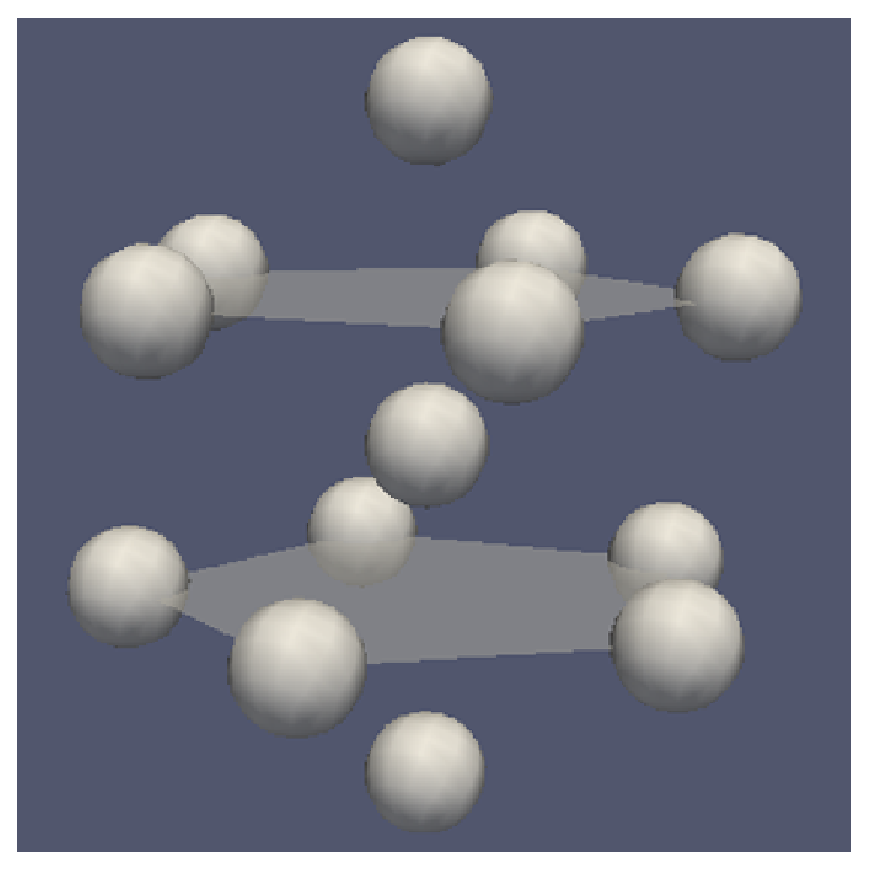
\includegraphics[width=0.22\textwidth]{ico_13}};
    	\node[below] at (ico.south) {Icosahedron};
    	\draw[dashed] (-0.0937, 0.3em) -- (-0.0937, 2em) node [inner sep=0pt,above right] (dodec){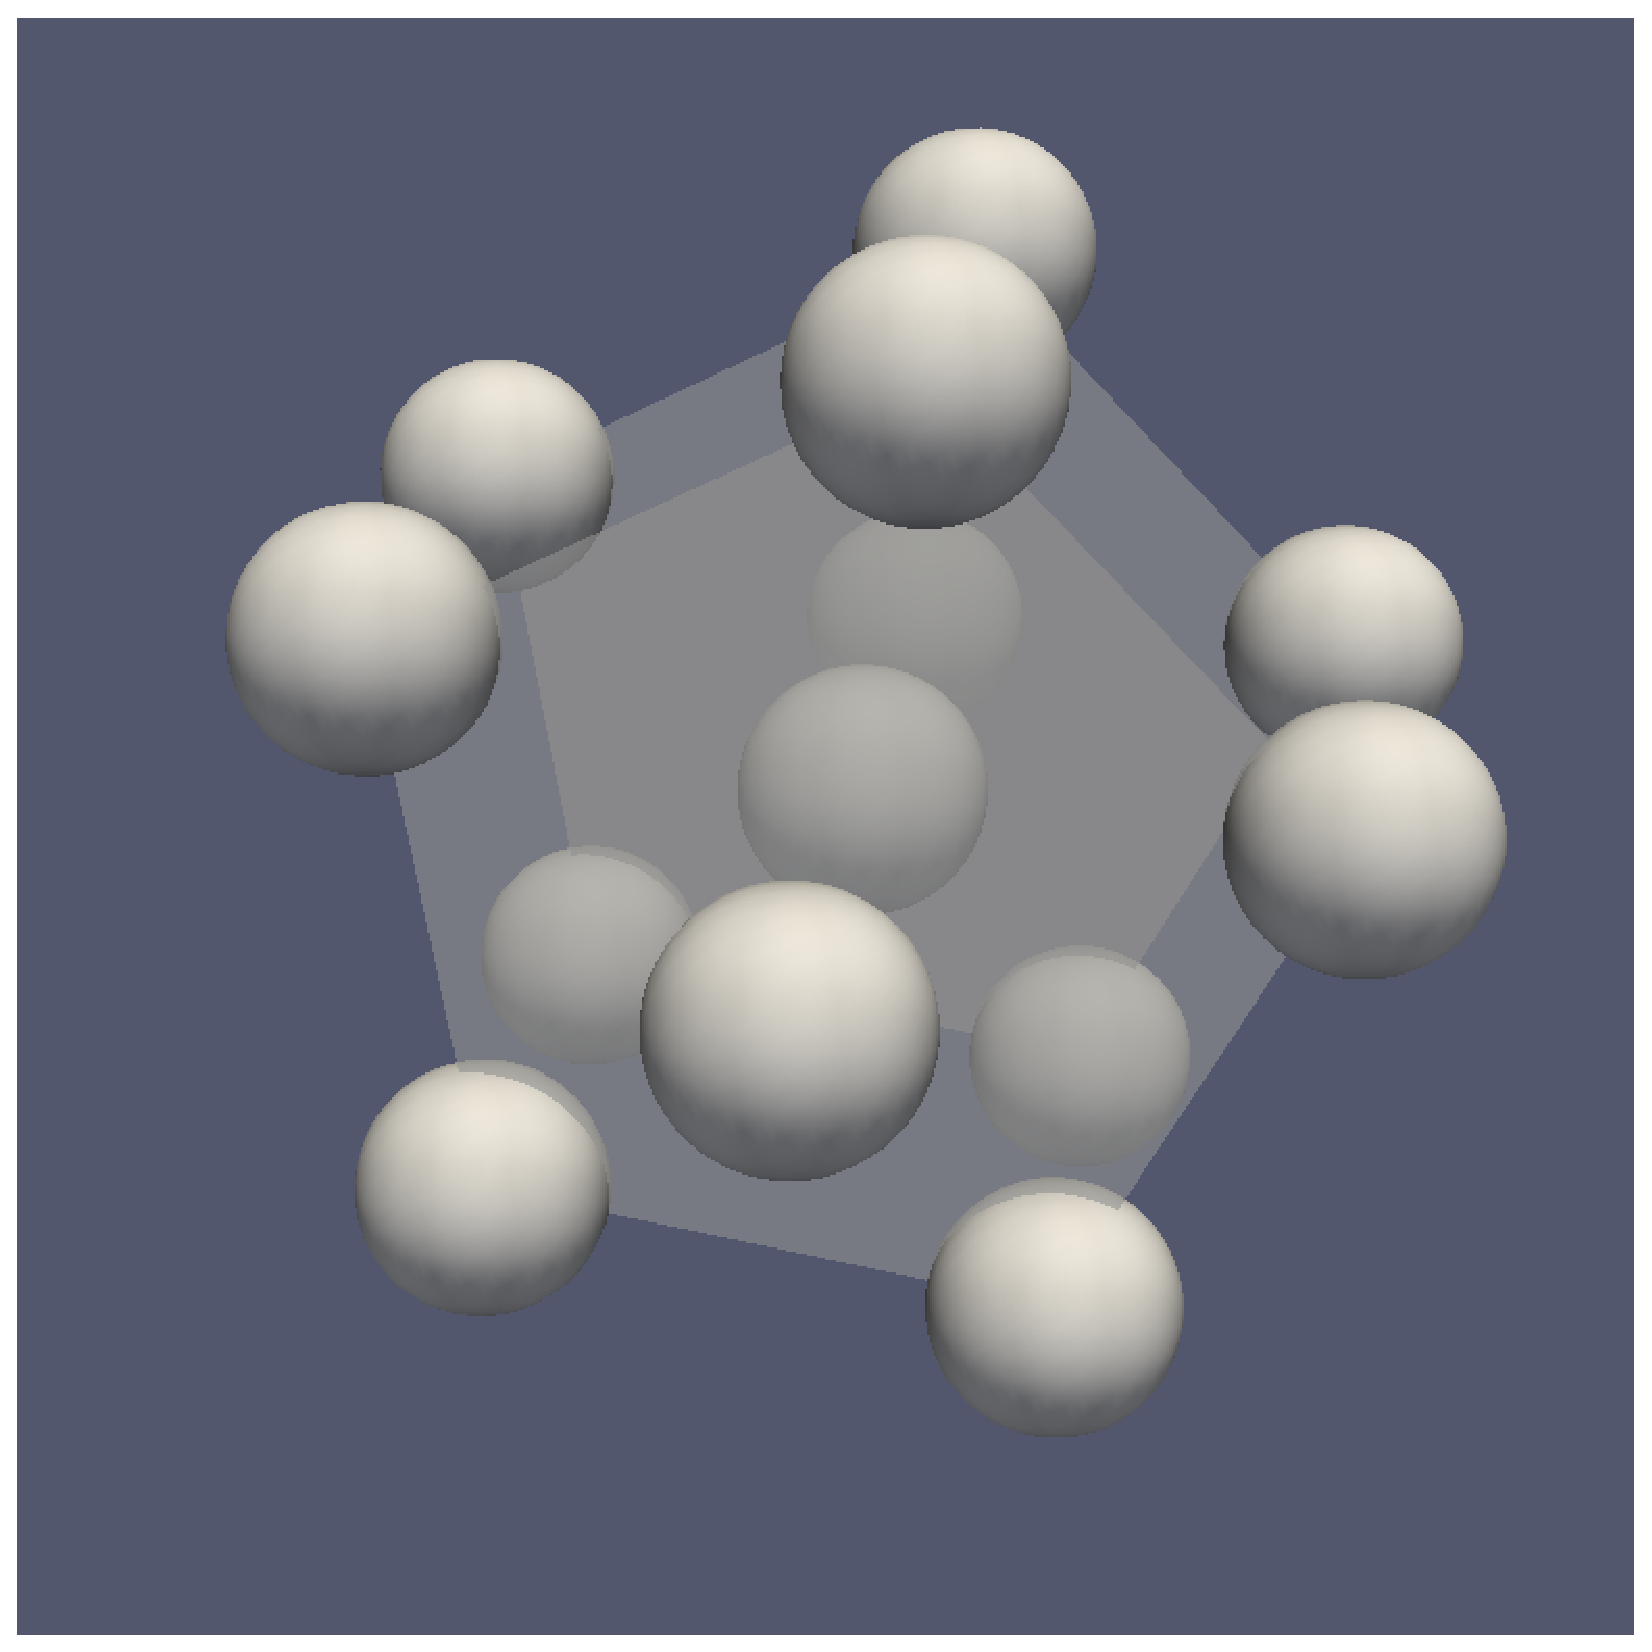
\includegraphics[width=0.22\textwidth]{dodec_13}};
    	\node[below] at (dodec.south) {Dodecahedron};
	\end{tikzpicture}
	
	\alt<all:1>{\begin{columns}
	\column{0.5\textwidth}
	$w_6^{ico}$ is the absolute minimum 
	\[ w_6^{ico}= -\frac{11}{\sqrt{4199}} \sim -0.1697 \]
	\column{0.5\textwidth}
	\begin{itemize}
		\item Icosahedra exist in attractive systems
		\item In hard spheres: only packing
		\item Not looked for except at $\phi>\phi_g$
	\end{itemize}
	\end{columns}}%
	{$w_6^* \simeq 0.15$ differentiate between
	\begin{itemize}
		\item perfect (stable) icosahedra
		\item imperfect (less stable) icosahedra
	\end{itemize}}
\end{frame}

\begin{frame}{Icosahedral order}
	\begin{textblock*}{0.6\textwidth}(10mm,92mm)
		\simplephasediagram{}
	\end{textblock*}
	\begin{columns}
	\column{0.65\textwidth}
	\resizebox{1.15\columnwidth}{!}{\input{w6Q6quarter.pdf_tex}}
	\column{0.35\textwidth}
	\begin{itemize}
		\item Already in the normal liquid
		\item Increases with supercooling
	\end{itemize}
	\end{columns}
\end{frame}

\begin{frame}<all:1->{Two types of orders in real space}
	\begin{textblock*}{0.6\textwidth}(10mm,92mm)
		\simplephasediagram{%
		\node<all:1> at (0.497,0) [xp marker, fill=green!50!black] {};
		\node<all:2> at (0.535,0) [xp marker, fill=green!50!black] {};
		\node<all:3> at (0.576,0) [xp marker, fill=green!50!black] {};
		}
	\end{textblock*}
	\begin{columns}[T]
	\column{0.6\textwidth}
	\only<all:1>{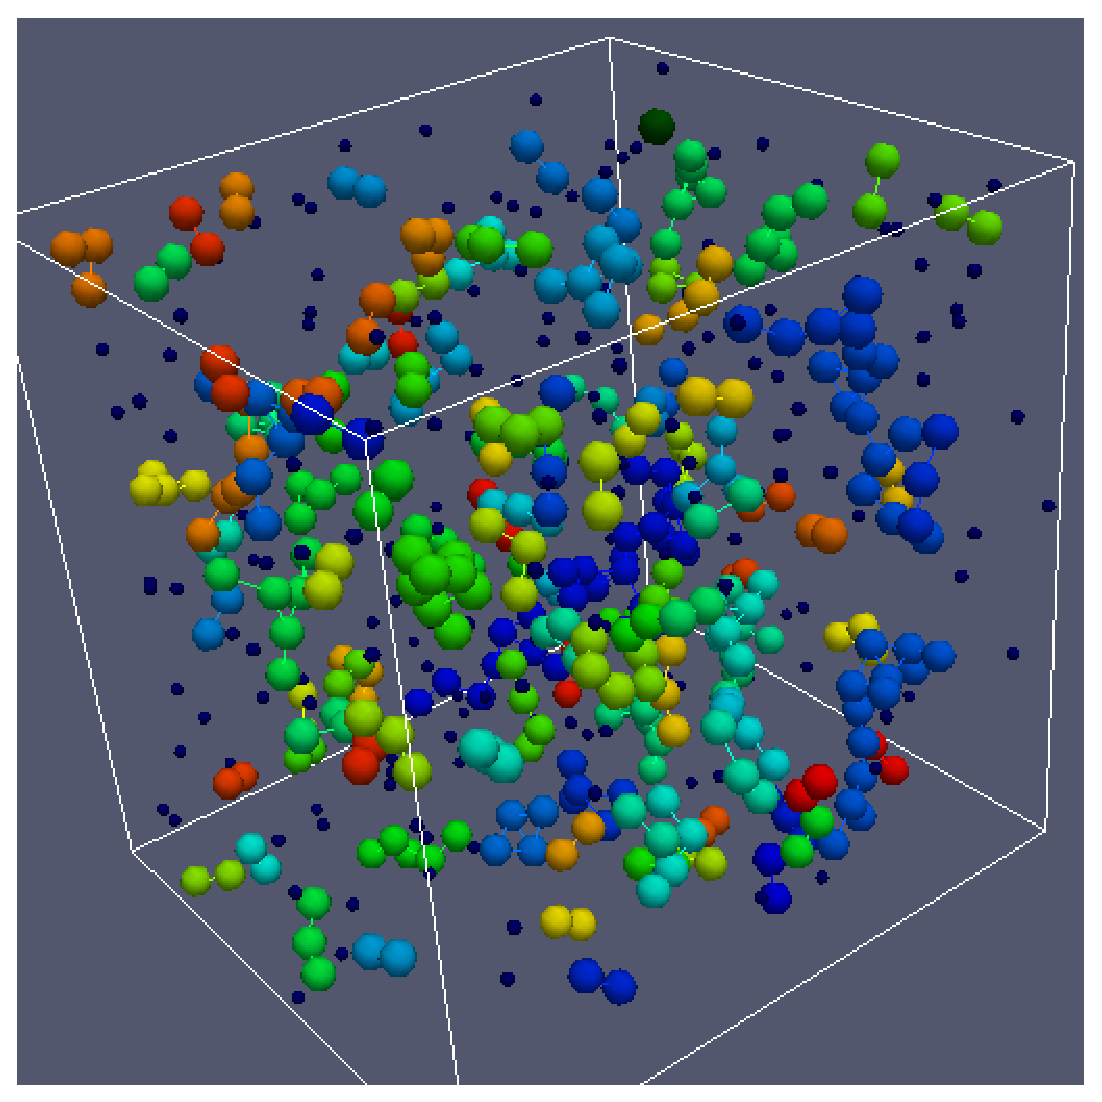
\includegraphics[width=\columnwidth]{mrco_alphabonds_3954}
	\[ \phi=0.497 \]}%
	\only<all:2>{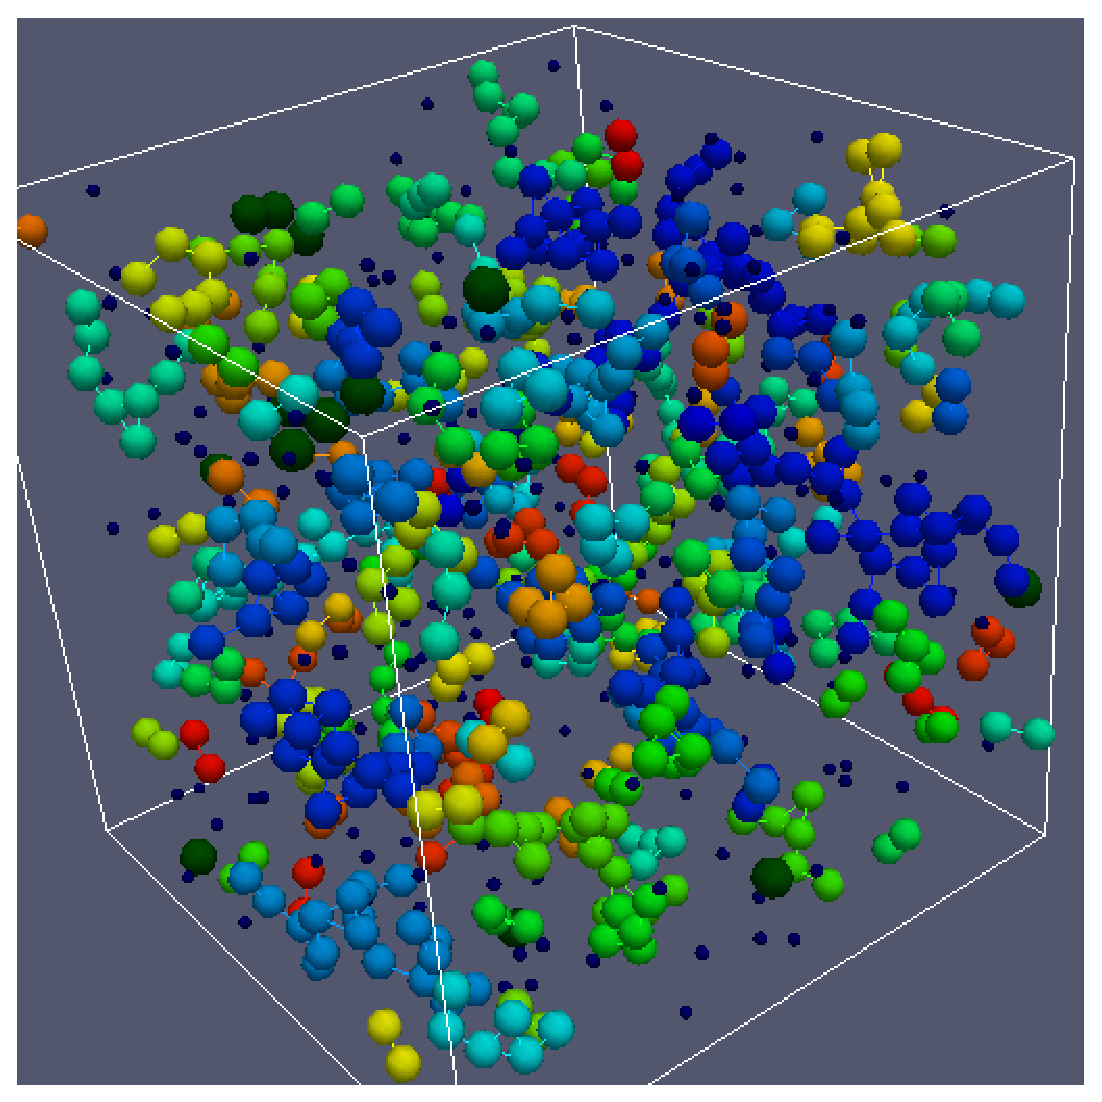
\includegraphics[width=\columnwidth]{mrco_alphabonds_4582}
	\[ \phi=0.535 \]}%
	\only<all:3>{\includegraphics[width=\columnwidth]{mrco_alphabonds_go1}
	\[ \phi=0.576 \]}%
	\column{0.4\textwidth}
	\begin{block}{Central particle}
	\begin{itemize}
		\item Crystal-like \tikz\shade[ball color=green!33!black] (0,0) circle (0.5em);
		\item Icosahedra 
		\begin{itemize}
			\item isolated \tikz\shade[ball color=blue!50!black] (0,0) circle (0.3em);
			\item connected \begin{tikzpicture}
				\shade[ball color=blue] (0,0) circle (0.5em);
				\shade[ball color=green] +(1em,0) circle (0.5em);
				\shade[ball color=yellow] +(2em,0) circle (0.5em);
				\shade[ball color=red] +(3em,0) circle (0.5em);
				\end{tikzpicture}
		\end{itemize}
	\end{itemize}
	\end{block}
	\begin{itemize}
		\item Crystal-like \only<all:1>{order negligible}%
			\only<all:2>{order forms clusters}%
			\only<all:3> {compact clusters growing}%
		\item Icosahedral \only<all:1>{order forms strings}%
			\only<all:2>{order forms low dimensional clusters}%
			\only<all:3>{network percolates}%
	\end{itemize}
	\end{columns}
\end{frame}

\subsection{Characterisation}

\begin{frame}<1-| handout:1,3>{Local volume fraction along the \alt<all:1>{crystal-like}{icosahedral} axis}
	\begin{textblock*}{0.6\textwidth}(10mm,92mm)
		\simplephasediagram{}
	\end{textblock*}
	\begin{columns}
	\column{0.3\textwidth}
	\begin{tikzpicture}[scale=0.13]
		\tikzset{particle/.style={circle, ball color=blue!50!white, inner sep=0, minimum size=1.5em}}
		\tikzset{vertice/.style={circle, ball color=red!50!white, inner sep=0}}
		\tikzset{edge/.style={thick, green!33!black}}
		\node [vertice] at (54.249, 39) (v2) {};
		\node [vertice] at (56.188, 41.909) (v3) {};
		\node [vertice] at (49.390, 43.713) (v5) {};
		\node [vertice] at (47.620, 45.446) (v6) {};
		\node [vertice] at (44.765, 45.106) (v7) {};
		\node [vertice] at (42.413, 47.493) (v8) {};
		\node [vertice] at (43.388, 50.418) (v9) {};
		\node [vertice] at (52.905, 53.618) (v10) {};
		\node [vertice] at (48.781, 49.134) (v11) {};
		\node [vertice] at (48.073, 55.602) (v12) {};
		\node [vertice] at (46.675, 51.240) (v13) {};
		\node [vertice] at (53.776, 45.093) (v14) {};
		\node [vertice] at (55.715, 43.8) (v15) {};
		\node [vertice] at (52.603, 49.531) (v16) {};
		\node [vertice] at (53.321, 50.608) (v17) {};
		\node [vertice] at (59.416, 47.5) (v18) {};
		\node [vertice] at (58.488, 50.283) (v19) {};
		\node [vertice] at (49.582, 39) (v20) {};
		\node [vertice] at (48.988, 39.891) (v21) {};
		\node [vertice] at (43.416, 40.682) (v23) {};
		\fill<all:1-2>[red!50!white] (v5.center) -- (v6.center) -- (v11.center) -- (v16.center) -- (v14.center) -- cycle;
		\fill<all:3>[red!50!white] (v2.center) -- (v3.center) -- (v15.center) -- (v18.center) -- (v19.center) -- (v17.center) -- (v10.center) -- (v12.center) -- (v13.center) -- (v9.center) -- (v8.center) -- (v7.center) -- (v23.center) -- (v21.center) -- (v20.center) -- cycle;
		\draw[edge] (v2.center) -- (v3.center) -- (v15.center) -- (v14.center) -- (v5.center) -- (v21.center) -- (v20.center) -- cycle;
		\draw[edge] (v5.center) -- (v6.center) -- (v7.center) -- (v23.center) -- (v21.center) -- cycle;
		\draw[edge] (v6.center) -- (v7.center) -- (v8.center) -- (v9.center) -- (v13.center) -- (v11.center) -- cycle;
		\draw[edge] (v11.center) -- (v16.center) -- (v17.center) -- (v10.center) -- (v12.center) -- (v13.center) -- cycle;
		\draw[edge] (v14.center) -- (v15.center) -- (v18.center) -- (v19.center) -- (v17.center) -- (v16.center) -- cycle;
		\node [particle] at (51.916, 56.871) (p1) {};
		\node [particle] at (44.480, 53.742) (p2) {};
		\node [particle] at (49.916, 52.000) (p3) {};
		\node [particle] at (56.222, 52.871) (p4) {};
		\node [particle] at (39.916, 50.000) (p5) {};
		\node [particle] at (45.916, 48.000) (p6) {};
		\node [particle] at (50.480, 46.564) (p7) {};
		\node [particle] at (55.916, 48.000) (p8) {};
		\node [particle] at (61.916, 50.000) (p9) {};
		\node [particle] at (41.854, 44.000) (p10) {};
		\node [particle] at (46.564, 42.564) (p11) {};
		\node [particle] at (51.916, 42.000) (p12) {};
		\node [particle] at (59.916, 44.000) (p13) {};
		\node [particle] at (45.916, 38.000) (p15) {};
		\node [particle] at (51.916, 36.000) (p16) {};
		\node [particle] at (57.916, 38.000) (p17) {};
	\end{tikzpicture}
	\column{0.7\textwidth}
	\resizebox{\columnwidth}{!}{%
		\only<all:1>{% GNUPLOT: LaTeX picture with Postscript
\begingroup
  \makeatletter
  \providecommand\color[2][]{%
    \GenericError{(gnuplot) \space\space\space\@spaces}{%
      Package color not loaded in conjunction with
      terminal option `colourtext'%
    }{See the gnuplot documentation for explanation.%
    }{Either use 'blacktext' in gnuplot or load the package
      color.sty in LaTeX.}%
    \renewcommand\color[2][]{}%
  }%
  \providecommand\includegraphics[2][]{%
    \GenericError{(gnuplot) \space\space\space\@spaces}{%
      Package graphicx or graphics not loaded%
    }{See the gnuplot documentation for explanation.%
    }{The gnuplot epslatex terminal needs graphicx.sty or graphics.sty.}%
    \renewcommand\includegraphics[2][]{}%
  }%
  \providecommand\rotatebox[2]{#2}%
  \@ifundefined{ifGPcolor}{%
    \newif\ifGPcolor
    \GPcolortrue
  }{}%
  \@ifundefined{ifGPblacktext}{%
    \newif\ifGPblacktext
    \GPblacktexttrue
  }{}%
  % define a \g@addto@macro without @ in the name:
  \let\gplgaddtomacro\g@addto@macro
  % define empty templates for all commands taking text:
  \gdef\gplbacktext{}%
  \gdef\gplfronttext{}%
  \makeatother
  \ifGPblacktext
    % no textcolor at all
    \def\colorrgb#1{}%
    \def\colorgray#1{}%
  \else
    % gray or color?
    \ifGPcolor
      \def\colorrgb#1{\color[rgb]{#1}}%
      \def\colorgray#1{\color[gray]{#1}}%
      \expandafter\def\csname LTw\endcsname{\color{white}}%
      \expandafter\def\csname LTb\endcsname{\color{black}}%
      \expandafter\def\csname LTa\endcsname{\color{black}}%
      \expandafter\def\csname LT0\endcsname{\color[rgb]{1,0,0}}%
      \expandafter\def\csname LT1\endcsname{\color[rgb]{0,1,0}}%
      \expandafter\def\csname LT2\endcsname{\color[rgb]{0,0,1}}%
      \expandafter\def\csname LT3\endcsname{\color[rgb]{1,0,1}}%
      \expandafter\def\csname LT4\endcsname{\color[rgb]{0,1,1}}%
      \expandafter\def\csname LT5\endcsname{\color[rgb]{1,1,0}}%
      \expandafter\def\csname LT6\endcsname{\color[rgb]{0,0,0}}%
      \expandafter\def\csname LT7\endcsname{\color[rgb]{1,0.3,0}}%
      \expandafter\def\csname LT8\endcsname{\color[rgb]{0.5,0.5,0.5}}%
    \else
      % gray
      \def\colorrgb#1{\color{black}}%
      \def\colorgray#1{\color[gray]{#1}}%
      \expandafter\def\csname LTw\endcsname{\color{white}}%
      \expandafter\def\csname LTb\endcsname{\color{black}}%
      \expandafter\def\csname LTa\endcsname{\color{black}}%
      \expandafter\def\csname LT0\endcsname{\color{black}}%
      \expandafter\def\csname LT1\endcsname{\color{black}}%
      \expandafter\def\csname LT2\endcsname{\color{black}}%
      \expandafter\def\csname LT3\endcsname{\color{black}}%
      \expandafter\def\csname LT4\endcsname{\color{black}}%
      \expandafter\def\csname LT5\endcsname{\color{black}}%
      \expandafter\def\csname LT6\endcsname{\color{black}}%
      \expandafter\def\csname LT7\endcsname{\color{black}}%
      \expandafter\def\csname LT8\endcsname{\color{black}}%
    \fi
  \fi
  \setlength{\unitlength}{0.0500bp}%
  \begin{picture}(7200.00,5040.00)%
    \gplgaddtomacro\gplbacktext{%
      \csname LTb\endcsname%
      \put(1056,2520){\makebox(0,0)[r]{\strut{}$0.4$}}%
      \put(1056,3165){\makebox(0,0)[r]{\strut{}$0.5$}}%
      \put(1056,3809){\makebox(0,0)[r]{\strut{}$0.6$}}%
      \put(1056,4454){\makebox(0,0)[r]{\strut{}$0.7$}}%
      \put(1188,2300){\makebox(0,0){\strut{}}}%
      \put(1931,2300){\makebox(0,0){\strut{}}}%
      \put(2674,2300){\makebox(0,0){\strut{}}}%
      \put(3417,2300){\makebox(0,0){\strut{}}}%
      \put(4160,2300){\makebox(0,0){\strut{}}}%
      \put(4903,2300){\makebox(0,0){\strut{}}}%
      \put(5646,2300){\makebox(0,0){\strut{}}}%
      \put(6389,2300){\makebox(0,0){\strut{}}}%
      \put(418,3648){\rotatebox{-270}{\makebox(0,0){\strut{}$<\tilde{\phi}_{local}>$}}}%
      \put(6979,3648){\rotatebox{-270}{\makebox(0,0){\strut{}}}}%
      \put(3974,4666){\makebox(0,0){\strut{}}}%
      \put(3974,4665){\makebox(0,0){\strut{}}}%
      \put(264,2410){\makebox(0,0)[l]{\strut{}}}%
    }%
    \gplgaddtomacro\gplfronttext{%
      \put(5424,4603){\makebox(0,0){\strut{}Experiments}}%
      \csname LTb\endcsname%
      \put(5805,3569){\makebox(0,0)[r]{\strut{}$\phi=0.497$}}%
      \csname LTb\endcsname%
      \put(5805,3833){\makebox(0,0)[r]{\strut{}$\phi=0.535$}}%
      \csname LTb\endcsname%
      \put(5805,4097){\makebox(0,0)[r]{\strut{}$\phi=0.555$}}%
      \csname LTb\endcsname%
      \put(5805,4361){\makebox(0,0)[r]{\strut{}$\phi=0.576$}}%
    }%
    \gplgaddtomacro\gplbacktext{%
      \csname LTb\endcsname%
      \put(1056,704){\makebox(0,0)[r]{\strut{}$0.4$}}%
      \put(1056,1223){\makebox(0,0)[r]{\strut{}$0.5$}}%
      \put(1056,1741){\makebox(0,0)[r]{\strut{}$0.6$}}%
      \put(1056,2260){\makebox(0,0)[r]{\strut{}$0.7$}}%
      \put(1188,484){\makebox(0,0){\strut{}$0$}}%
      \put(1931,484){\makebox(0,0){\strut{}$0.1$}}%
      \put(2674,484){\makebox(0,0){\strut{}$0.2$}}%
      \put(3417,484){\makebox(0,0){\strut{}$0.3$}}%
      \put(4160,484){\makebox(0,0){\strut{}$0.4$}}%
      \put(4903,484){\makebox(0,0){\strut{}$0.5$}}%
      \put(5646,484){\makebox(0,0){\strut{}$0.6$}}%
      \put(6389,484){\makebox(0,0){\strut{}$0.7$}}%
      \put(418,1611){\rotatebox{-270}{\makebox(0,0){\strut{}$<\phi_{local}>$}}}%
      \put(6979,1611){\rotatebox{-270}{\makebox(0,0){\strut{}}}}%
      \put(3974,154){\makebox(0,0){\strut{}$Q_6$}}%
      \put(3974,2409){\makebox(0,0){\strut{}}}%
      \put(3974,2408){\makebox(0,0){\strut{}}}%
      \put(264,110){\makebox(0,0)[l]{\strut{}}}%
    }%
    \gplgaddtomacro\gplfronttext{%
      \put(5358,2346){\makebox(0,0){\strut{}Simulations}}%
      \csname LTb\endcsname%
      \put(5805,1048){\makebox(0,0)[r]{\strut{}$\phi=0.487$ }}%
      \csname LTb\endcsname%
      \put(5805,1312){\makebox(0,0)[r]{\strut{}$\phi=0.507$ }}%
      \csname LTb\endcsname%
      \put(5805,1576){\makebox(0,0)[r]{\strut{}$\phi=0.528$ }}%
      \csname LTb\endcsname%
      \put(5805,1840){\makebox(0,0)[r]{\strut{}$\phi=0.548$ }}%
      \csname LTb\endcsname%
      \put(5805,2104){\makebox(0,0)[r]{\strut{}$\phi=0.568$ }}%
    }%
    \gplbacktext
    \put(0,0){\includegraphics{phi_Q6_xpsim}}%
    \gplfronttext
  \end{picture}%
\endgroup
}%
		\only<all:2>{% GNUPLOT: LaTeX picture with Postscript
\begingroup
  \makeatletter
  \providecommand\color[2][]{%
    \GenericError{(gnuplot) \space\space\space\@spaces}{%
      Package color not loaded in conjunction with
      terminal option `colourtext'%
    }{See the gnuplot documentation for explanation.%
    }{Either use 'blacktext' in gnuplot or load the package
      color.sty in LaTeX.}%
    \renewcommand\color[2][]{}%
  }%
  \providecommand\includegraphics[2][]{%
    \GenericError{(gnuplot) \space\space\space\@spaces}{%
      Package graphicx or graphics not loaded%
    }{See the gnuplot documentation for explanation.%
    }{The gnuplot epslatex terminal needs graphicx.sty or graphics.sty.}%
    \renewcommand\includegraphics[2][]{}%
  }%
  \providecommand\rotatebox[2]{#2}%
  \@ifundefined{ifGPcolor}{%
    \newif\ifGPcolor
    \GPcolortrue
  }{}%
  \@ifundefined{ifGPblacktext}{%
    \newif\ifGPblacktext
    \GPblacktexttrue
  }{}%
  % define a \g@addto@macro without @ in the name:
  \let\gplgaddtomacro\g@addto@macro
  % define empty templates for all commands taking text:
  \gdef\gplbacktext{}%
  \gdef\gplfronttext{}%
  \makeatother
  \ifGPblacktext
    % no textcolor at all
    \def\colorrgb#1{}%
    \def\colorgray#1{}%
  \else
    % gray or color?
    \ifGPcolor
      \def\colorrgb#1{\color[rgb]{#1}}%
      \def\colorgray#1{\color[gray]{#1}}%
      \expandafter\def\csname LTw\endcsname{\color{white}}%
      \expandafter\def\csname LTb\endcsname{\color{black}}%
      \expandafter\def\csname LTa\endcsname{\color{black}}%
      \expandafter\def\csname LT0\endcsname{\color[rgb]{1,0,0}}%
      \expandafter\def\csname LT1\endcsname{\color[rgb]{0,1,0}}%
      \expandafter\def\csname LT2\endcsname{\color[rgb]{0,0,1}}%
      \expandafter\def\csname LT3\endcsname{\color[rgb]{1,0,1}}%
      \expandafter\def\csname LT4\endcsname{\color[rgb]{0,1,1}}%
      \expandafter\def\csname LT5\endcsname{\color[rgb]{1,1,0}}%
      \expandafter\def\csname LT6\endcsname{\color[rgb]{0,0,0}}%
      \expandafter\def\csname LT7\endcsname{\color[rgb]{1,0.3,0}}%
      \expandafter\def\csname LT8\endcsname{\color[rgb]{0.5,0.5,0.5}}%
    \else
      % gray
      \def\colorrgb#1{\color{black}}%
      \def\colorgray#1{\color[gray]{#1}}%
      \expandafter\def\csname LTw\endcsname{\color{white}}%
      \expandafter\def\csname LTb\endcsname{\color{black}}%
      \expandafter\def\csname LTa\endcsname{\color{black}}%
      \expandafter\def\csname LT0\endcsname{\color{black}}%
      \expandafter\def\csname LT1\endcsname{\color{black}}%
      \expandafter\def\csname LT2\endcsname{\color{black}}%
      \expandafter\def\csname LT3\endcsname{\color{black}}%
      \expandafter\def\csname LT4\endcsname{\color{black}}%
      \expandafter\def\csname LT5\endcsname{\color{black}}%
      \expandafter\def\csname LT6\endcsname{\color{black}}%
      \expandafter\def\csname LT7\endcsname{\color{black}}%
      \expandafter\def\csname LT8\endcsname{\color{black}}%
    \fi
  \fi
  \setlength{\unitlength}{0.0500bp}%
  \begin{picture}(7200.00,5040.00)%
    \gplgaddtomacro\gplbacktext{%
      \csname LTb\endcsname%
      \put(1056,2520){\makebox(0,0)[r]{\strut{}$0.4$}}%
      \put(1056,3165){\makebox(0,0)[r]{\strut{}$0.5$}}%
      \put(1056,3809){\makebox(0,0)[r]{\strut{}$0.6$}}%
      \put(1056,4454){\makebox(0,0)[r]{\strut{}$0.7$}}%
      \put(1369,2300){\makebox(0,0){\strut{}}}%
      \put(1791,2300){\makebox(0,0){\strut{}}}%
      \put(2394,2300){\makebox(0,0){\strut{}}}%
      \put(2997,2300){\makebox(0,0){\strut{}}}%
      \put(418,3648){\rotatebox{-270}{\makebox(0,0){\strut{}$<\tilde{\phi}_{local}>$}}}%
      \put(3819,3648){\rotatebox{-270}{\makebox(0,0){\strut{}}}}%
      \put(2394,4666){\makebox(0,0){\strut{}}}%
      \put(2394,4665){\makebox(0,0){\strut{}}}%
      \put(264,2190){\makebox(0,0)[l]{\strut{}}}%
    }%
    \gplgaddtomacro\gplfronttext{%
      \put(2557,4537){\makebox(0,0){\strut{}Experiments}}%
    }%
    \gplgaddtomacro\gplbacktext{%
      \csname LTb\endcsname%
      \put(6231,3648){\rotatebox{-270}{\makebox(0,0){\strut{} }}}%
      \put(4806,4666){\makebox(0,0){\strut{}}}%
      \put(4806,4665){\makebox(0,0){\strut{}}}%
      \put(3600,2630){\makebox(0,0)[l]{\strut{}}}%
    }%
    \gplgaddtomacro\gplfronttext{%
      \csname LTb\endcsname%
      \put(4669,3877){\makebox(0,0)[r]{\strut{}$\phi=0.497$}}%
      \csname LTb\endcsname%
      \put(4669,4097){\makebox(0,0)[r]{\strut{}$\phi=0.535$}}%
      \csname LTb\endcsname%
      \put(4669,4317){\makebox(0,0)[r]{\strut{}$\phi=0.555$}}%
      \csname LTb\endcsname%
      \put(4669,4537){\makebox(0,0)[r]{\strut{}$\phi=0.576$}}%
    }%
    \gplgaddtomacro\gplbacktext{%
      \csname LTb\endcsname%
      \put(1056,704){\makebox(0,0)[r]{\strut{}$0.4$}}%
      \put(1056,1223){\makebox(0,0)[r]{\strut{}$0.5$}}%
      \put(1056,1741){\makebox(0,0)[r]{\strut{}$0.6$}}%
      \put(1056,2260){\makebox(0,0)[r]{\strut{}$0.7$}}%
      \put(1369,484){\makebox(0,0){\strut{}$-0.17$}}%
      \put(1791,484){\makebox(0,0){\strut{}$-0.1$}}%
      \put(2394,484){\makebox(0,0){\strut{}$0$}}%
      \put(2997,484){\makebox(0,0){\strut{}$0.1$}}%
      \put(418,1611){\rotatebox{90}{\makebox(0,0){\strut{}$<\phi_{local}>$}}}%
      \put(2394,154){\makebox(0,0){\strut{}$w_6$}}%
      \put(2394,2409){\makebox(0,0){\strut{}}}%
      \put(2394,2408){\makebox(0,0){\strut{}}}%
      \put(264,110){\makebox(0,0)[l]{\strut{}}}%
    }%
    \gplgaddtomacro\gplfronttext{%
      \put(2161,2305){\makebox(0,0){\strut{}Simulations}}%
      \csname LTb\endcsname%
      \put(2740,1865){\makebox(0,0)[r]{\strut{}$\phi=0.548$ }}%
      \csname LTb\endcsname%
      \put(2740,2085){\makebox(0,0)[r]{\strut{}$\phi=0.568$ }}%
    }%
    \gplgaddtomacro\gplbacktext{%
      \csname LTb\endcsname%
      \put(6231,1611){\rotatebox{90}{\makebox(0,0){\strut{} }}}%
      \put(4806,2409){\makebox(0,0){\strut{}}}%
      \put(4806,2408){\makebox(0,0){\strut{}}}%
      \put(3600,814){\makebox(0,0)[l]{\strut{}}}%
    }%
    \gplgaddtomacro\gplfronttext{%
      \csname LTb\endcsname%
      \put(4669,1865){\makebox(0,0)[r]{\strut{}$\phi=0.487$ }}%
      \csname LTb\endcsname%
      \put(4669,2085){\makebox(0,0)[r]{\strut{}$\phi=0.507$ }}%
      \csname LTb\endcsname%
      \put(4669,2305){\makebox(0,0)[r]{\strut{}$\phi=0.528$ }}%
    }%
    \gplbacktext
    \put(0,0){\includegraphics{phi_w6_xpsim_local}}%
    \gplfronttext
  \end{picture}%
\endgroup
}%
		\only<all:3>{% GNUPLOT: LaTeX picture with Postscript
\begingroup
  \makeatletter
  \providecommand\color[2][]{%
    \GenericError{(gnuplot) \space\space\space\@spaces}{%
      Package color not loaded in conjunction with
      terminal option `colourtext'%
    }{See the gnuplot documentation for explanation.%
    }{Either use 'blacktext' in gnuplot or load the package
      color.sty in LaTeX.}%
    \renewcommand\color[2][]{}%
  }%
  \providecommand\includegraphics[2][]{%
    \GenericError{(gnuplot) \space\space\space\@spaces}{%
      Package graphicx or graphics not loaded%
    }{See the gnuplot documentation for explanation.%
    }{The gnuplot epslatex terminal needs graphicx.sty or graphics.sty.}%
    \renewcommand\includegraphics[2][]{}%
  }%
  \providecommand\rotatebox[2]{#2}%
  \@ifundefined{ifGPcolor}{%
    \newif\ifGPcolor
    \GPcolortrue
  }{}%
  \@ifundefined{ifGPblacktext}{%
    \newif\ifGPblacktext
    \GPblacktexttrue
  }{}%
  % define a \g@addto@macro without @ in the name:
  \let\gplgaddtomacro\g@addto@macro
  % define empty templates for all commands taking text:
  \gdef\gplbacktext{}%
  \gdef\gplfronttext{}%
  \makeatother
  \ifGPblacktext
    % no textcolor at all
    \def\colorrgb#1{}%
    \def\colorgray#1{}%
  \else
    % gray or color?
    \ifGPcolor
      \def\colorrgb#1{\color[rgb]{#1}}%
      \def\colorgray#1{\color[gray]{#1}}%
      \expandafter\def\csname LTw\endcsname{\color{white}}%
      \expandafter\def\csname LTb\endcsname{\color{black}}%
      \expandafter\def\csname LTa\endcsname{\color{black}}%
      \expandafter\def\csname LT0\endcsname{\color[rgb]{1,0,0}}%
      \expandafter\def\csname LT1\endcsname{\color[rgb]{0,1,0}}%
      \expandafter\def\csname LT2\endcsname{\color[rgb]{0,0,1}}%
      \expandafter\def\csname LT3\endcsname{\color[rgb]{1,0,1}}%
      \expandafter\def\csname LT4\endcsname{\color[rgb]{0,1,1}}%
      \expandafter\def\csname LT5\endcsname{\color[rgb]{1,1,0}}%
      \expandafter\def\csname LT6\endcsname{\color[rgb]{0,0,0}}%
      \expandafter\def\csname LT7\endcsname{\color[rgb]{1,0.3,0}}%
      \expandafter\def\csname LT8\endcsname{\color[rgb]{0.5,0.5,0.5}}%
    \else
      % gray
      \def\colorrgb#1{\color{black}}%
      \def\colorgray#1{\color[gray]{#1}}%
      \expandafter\def\csname LTw\endcsname{\color{white}}%
      \expandafter\def\csname LTb\endcsname{\color{black}}%
      \expandafter\def\csname LTa\endcsname{\color{black}}%
      \expandafter\def\csname LT0\endcsname{\color{black}}%
      \expandafter\def\csname LT1\endcsname{\color{black}}%
      \expandafter\def\csname LT2\endcsname{\color{black}}%
      \expandafter\def\csname LT3\endcsname{\color{black}}%
      \expandafter\def\csname LT4\endcsname{\color{black}}%
      \expandafter\def\csname LT5\endcsname{\color{black}}%
      \expandafter\def\csname LT6\endcsname{\color{black}}%
      \expandafter\def\csname LT7\endcsname{\color{black}}%
      \expandafter\def\csname LT8\endcsname{\color{black}}%
    \fi
  \fi
  \setlength{\unitlength}{0.0500bp}%
  \begin{picture}(7200.00,5040.00)%
    \gplgaddtomacro\gplbacktext{%
      \csname LTb\endcsname%
      \put(1056,2520){\makebox(0,0)[r]{\strut{}$0.4$}}%
      \put(1056,3165){\makebox(0,0)[r]{\strut{}$0.5$}}%
      \put(1056,3809){\makebox(0,0)[r]{\strut{}$0.6$}}%
      \put(1056,4454){\makebox(0,0)[r]{\strut{}$0.7$}}%
      \put(1369,2300){\makebox(0,0){\strut{}}}%
      \put(1791,2300){\makebox(0,0){\strut{}}}%
      \put(2394,2300){\makebox(0,0){\strut{}}}%
      \put(2997,2300){\makebox(0,0){\strut{}}}%
      \put(418,3648){\rotatebox{-270}{\makebox(0,0){\strut{}$<\tilde{\phi}_{local}>$}}}%
      \put(3819,3648){\rotatebox{-270}{\makebox(0,0){\strut{}}}}%
      \put(2394,4666){\makebox(0,0){\strut{}}}%
      \put(2394,4665){\makebox(0,0){\strut{}}}%
      \put(264,2190){\makebox(0,0)[l]{\strut{}}}%
    }%
    \gplgaddtomacro\gplfronttext{%
      \put(2557,4537){\makebox(0,0){\strut{}Experiments}}%
    }%
    \gplgaddtomacro\gplbacktext{%
      \csname LTb\endcsname%
      \put(3468,2520){\makebox(0,0)[r]{\strut{}}}%
      \put(3468,3165){\makebox(0,0)[r]{\strut{}}}%
      \put(3468,3809){\makebox(0,0)[r]{\strut{}}}%
      \put(3468,4454){\makebox(0,0)[r]{\strut{}}}%
      \put(3781,2300){\makebox(0,0){\strut{}}}%
      \put(4203,2300){\makebox(0,0){\strut{}}}%
      \put(4806,2300){\makebox(0,0){\strut{}}}%
      \put(5409,2300){\makebox(0,0){\strut{}}}%
      \put(6231,3648){\rotatebox{-270}{\makebox(0,0){\strut{}$<\tilde{\phi}_{ngb}>$}}}%
      \put(4806,4666){\makebox(0,0){\strut{}}}%
      \put(4806,4665){\makebox(0,0){\strut{}}}%
      \put(3336,2190){\makebox(0,0)[l]{\strut{}}}%
    }%
    \gplgaddtomacro\gplfronttext{%
      \csname LTb\endcsname%
      \put(4669,3877){\makebox(0,0)[r]{\strut{}$\phi=0.497$}}%
      \csname LTb\endcsname%
      \put(4669,4097){\makebox(0,0)[r]{\strut{}$\phi=0.535$}}%
      \csname LTb\endcsname%
      \put(4669,4317){\makebox(0,0)[r]{\strut{}$\phi=0.555$}}%
      \csname LTb\endcsname%
      \put(4669,4537){\makebox(0,0)[r]{\strut{}$\phi=0.576$}}%
    }%
    \gplgaddtomacro\gplbacktext{%
      \csname LTb\endcsname%
      \put(1056,704){\makebox(0,0)[r]{\strut{}$0.4$}}%
      \put(1056,1223){\makebox(0,0)[r]{\strut{}$0.5$}}%
      \put(1056,1741){\makebox(0,0)[r]{\strut{}$0.6$}}%
      \put(1056,2260){\makebox(0,0)[r]{\strut{}$0.7$}}%
      \put(1369,484){\makebox(0,0){\strut{}$-0.17$}}%
      \put(1791,484){\makebox(0,0){\strut{}$-0.1$}}%
      \put(2394,484){\makebox(0,0){\strut{}$0$}}%
      \put(2997,484){\makebox(0,0){\strut{}$0.1$}}%
      \put(418,1611){\rotatebox{90}{\makebox(0,0){\strut{}$<\phi_{local}>$}}}%
      \put(2394,154){\makebox(0,0){\strut{}$w_6$}}%
      \put(2394,2409){\makebox(0,0){\strut{}}}%
      \put(2394,2408){\makebox(0,0){\strut{}}}%
      \put(264,110){\makebox(0,0)[l]{\strut{}}}%
    }%
    \gplgaddtomacro\gplfronttext{%
      \put(2161,2305){\makebox(0,0){\strut{}Simulations}}%
      \csname LTb\endcsname%
      \put(2740,1865){\makebox(0,0)[r]{\strut{}$\phi=0.548$ }}%
      \csname LTb\endcsname%
      \put(2740,2085){\makebox(0,0)[r]{\strut{}$\phi=0.568$ }}%
    }%
    \gplgaddtomacro\gplbacktext{%
      \csname LTb\endcsname%
      \put(3468,704){\makebox(0,0)[r]{\strut{}}}%
      \put(3468,1223){\makebox(0,0)[r]{\strut{}}}%
      \put(3468,1741){\makebox(0,0)[r]{\strut{}}}%
      \put(3468,2260){\makebox(0,0)[r]{\strut{}}}%
      \put(3781,484){\makebox(0,0){\strut{}$-0.17$}}%
      \put(4203,484){\makebox(0,0){\strut{}$-0.1$}}%
      \put(4806,484){\makebox(0,0){\strut{}$0$}}%
      \put(5409,484){\makebox(0,0){\strut{}$0.1$}}%
      \put(6231,1611){\rotatebox{90}{\makebox(0,0){\strut{}$<\phi_{ngb}>$}}}%
      \put(4806,154){\makebox(0,0){\strut{}$w_6$}}%
      \put(4806,2409){\makebox(0,0){\strut{}}}%
      \put(4806,2408){\makebox(0,0){\strut{}}}%
      \put(3336,110){\makebox(0,0)[l]{\strut{}}}%
    }%
    \gplgaddtomacro\gplfronttext{%
      \csname LTb\endcsname%
      \put(4669,1865){\makebox(0,0)[r]{\strut{}$\phi=0.487$ }}%
      \csname LTb\endcsname%
      \put(4669,2085){\makebox(0,0)[r]{\strut{}$\phi=0.507$ }}%
      \csname LTb\endcsname%
      \put(4669,2305){\makebox(0,0)[r]{\strut{}$\phi=0.528$ }}%
    }%
    \gplbacktext
    \put(0,0){\includegraphics{phi_w6_xpsim_total}}%
    \gplfronttext
  \end{picture}%
\endgroup
}%
	}
	\end{columns}
	\alt<all:1>{%
	\begin{itemize}
		\item Crystallisation is a first order transition
		\item No steep change in density upon ordering
		\item Crystal-like bond ordered regions $\neq$ crystal
	\end{itemize}
	}{%
	\begin{itemize}
		\item Icosahedron's central particle has less free volume
		\item<3> Neighbours have more free volume $\Rightarrow$ stabilised
		\item<3> Much more stable below $w_6^* \simeq -0.15$
	\end{itemize}
	}%
\end{frame}

\againframe<all:2>{ico_axis}

\begin{frame}<all:1->{Perfect/imperfect icosahedra}
	\begin{textblock*}{0.6\textwidth}(10mm,92mm)
		\simplephasediagram{%
		\node<all:1> at (0.497,0) [xp marker, fill=green!50!black] {};
		\node<all:2> at (0.535,0) [xp marker, fill=green!50!black] {};
		\node<all:3> at (0.576,0) [xp marker, fill=green!50!black] {};
		}
	\end{textblock*}
	\begin{columns}[T]
	\column{0.6\textwidth}
	\only<all:1>{\includegraphics[width=\columnwidth]{stable_ico_3954}
	\[ \phi=0.497 \]}%
	\only<all:2>{\includegraphics[width=\columnwidth]{stable_ico_4582}
	\[ \phi=0.535 \]}%
	\only<all:3>{\includegraphics[width=\columnwidth]{stable_ico_go1}
	\[ \phi=0.576 \]}%
	\column{0.4\textwidth}
	\begin{block}{Central particle}
	\begin{itemize}
		\item Perfect \tikz\shade[ball color=gray] (0,0) circle (0.5em);
		\item Imperfect \tikz\shade[ball color=gray] (0,0) circle (0.3em);
	\end{itemize}
	\end{block}
	\begin{itemize}
		\item Perfect icosahedra are few 
		\item No medium range size without the imperfect icosahedra
	\end{itemize}
	\end{columns}
\end{frame}

\begin{frame}{Size of the crystal-like ordered regions}
	\begin{textblock*}{0.6\textwidth}(10mm,92mm)
		\simplephasediagram{}
	\end{textblock*}
	\centering\resizebox{0.5\textwidth}{!}{\begin{LARGE}% GNUPLOT: LaTeX picture with Postscript
\begingroup
  \makeatletter
  \providecommand\color[2][]{%
    \GenericError{(gnuplot) \space\space\space\@spaces}{%
      Package color not loaded in conjunction with
      terminal option `colourtext'%
    }{See the gnuplot documentation for explanation.%
    }{Either use 'blacktext' in gnuplot or load the package
      color.sty in LaTeX.}%
    \renewcommand\color[2][]{}%
  }%
  \providecommand\includegraphics[2][]{%
    \GenericError{(gnuplot) \space\space\space\@spaces}{%
      Package graphicx or graphics not loaded%
    }{See the gnuplot documentation for explanation.%
    }{The gnuplot epslatex terminal needs graphicx.sty or graphics.sty.}%
    \renewcommand\includegraphics[2][]{}%
  }%
  \providecommand\rotatebox[2]{#2}%
  \@ifundefined{ifGPcolor}{%
    \newif\ifGPcolor
    \GPcolortrue
  }{}%
  \@ifundefined{ifGPblacktext}{%
    \newif\ifGPblacktext
    \GPblacktexttrue
  }{}%
  % define a \g@addto@macro without @ in the name:
  \let\gplgaddtomacro\g@addto@macro
  % define empty templates for all commands taking text:
  \gdef\gplbacktext{}%
  \gdef\gplfronttext{}%
  \makeatother
  \ifGPblacktext
    % no textcolor at all
    \def\colorrgb#1{}%
    \def\colorgray#1{}%
  \else
    % gray or color?
    \ifGPcolor
      \def\colorrgb#1{\color[rgb]{#1}}%
      \def\colorgray#1{\color[gray]{#1}}%
      \expandafter\def\csname LTw\endcsname{\color{white}}%
      \expandafter\def\csname LTb\endcsname{\color{black}}%
      \expandafter\def\csname LTa\endcsname{\color{black}}%
      \expandafter\def\csname LT0\endcsname{\color[rgb]{1,0,0}}%
      \expandafter\def\csname LT1\endcsname{\color[rgb]{0,1,0}}%
      \expandafter\def\csname LT2\endcsname{\color[rgb]{0,0,1}}%
      \expandafter\def\csname LT3\endcsname{\color[rgb]{1,0,1}}%
      \expandafter\def\csname LT4\endcsname{\color[rgb]{0,1,1}}%
      \expandafter\def\csname LT5\endcsname{\color[rgb]{1,1,0}}%
      \expandafter\def\csname LT6\endcsname{\color[rgb]{0,0,0}}%
      \expandafter\def\csname LT7\endcsname{\color[rgb]{1,0.3,0}}%
      \expandafter\def\csname LT8\endcsname{\color[rgb]{0.5,0.5,0.5}}%
    \else
      % gray
      \def\colorrgb#1{\color{black}}%
      \def\colorgray#1{\color[gray]{#1}}%
      \expandafter\def\csname LTw\endcsname{\color{white}}%
      \expandafter\def\csname LTb\endcsname{\color{black}}%
      \expandafter\def\csname LTa\endcsname{\color{black}}%
      \expandafter\def\csname LT0\endcsname{\color{black}}%
      \expandafter\def\csname LT1\endcsname{\color{black}}%
      \expandafter\def\csname LT2\endcsname{\color{black}}%
      \expandafter\def\csname LT3\endcsname{\color{black}}%
      \expandafter\def\csname LT4\endcsname{\color{black}}%
      \expandafter\def\csname LT5\endcsname{\color{black}}%
      \expandafter\def\csname LT6\endcsname{\color{black}}%
      \expandafter\def\csname LT7\endcsname{\color{black}}%
      \expandafter\def\csname LT8\endcsname{\color{black}}%
    \fi
  \fi
  \setlength{\unitlength}{0.0500bp}%
  \begin{picture}(7200.00,5040.00)%
    \gplgaddtomacro\gplbacktext{%
      \csname LTb\endcsname%
      \put(1056,704){\makebox(0,0)[r]{\strut{}$10^{-7}$}}%
      \put(1056,1518){\makebox(0,0)[r]{\strut{}$10^{-6}$}}%
      \put(1056,2333){\makebox(0,0)[r]{\strut{}$10^{-5}$}}%
      \put(1056,3147){\makebox(0,0)[r]{\strut{}$10^{-4}$}}%
      \put(1056,3962){\makebox(0,0)[r]{\strut{}$10^{-3}$}}%
      \put(1056,4776){\makebox(0,0)[r]{\strut{}$10^{-2}$}}%
      \put(1453,484){\makebox(0,0){\strut{}$2$}}%
      \put(2117,484){\makebox(0,0){\strut{}$2.5$}}%
      \put(2780,484){\makebox(0,0){\strut{}$3$}}%
      \put(3443,484){\makebox(0,0){\strut{}$3.5$}}%
      \put(4107,484){\makebox(0,0){\strut{}$4$}}%
      \put(4770,484){\makebox(0,0){\strut{}$4.5$}}%
      \put(5433,484){\makebox(0,0){\strut{}$5$}}%
      \put(6097,484){\makebox(0,0){\strut{}$5.5$}}%
      \put(6760,484){\makebox(0,0){\strut{}$6$}}%
      \put(286,2740){\rotatebox{-270}{\makebox(0,0){\strut{}$G_6(r)$}}}%
      \put(6979,2740){\rotatebox{-270}{\makebox(0,0){\strut{}}}}%
      \put(3974,154){\makebox(0,0){\strut{}$r/\sigma$}}%
      \put(3974,4666){\makebox(0,0){\strut{}}}%
      \put(3974,4665){\makebox(0,0){\strut{}}}%
      \put(-264,110){\makebox(0,0)[l]{\strut{}}}%
    }%
    \gplgaddtomacro\gplfronttext{%
      \csname LTb\endcsname%
      \put(2904,932){\makebox(0,0)[r]{\strut{}$\phi=0.535$}}%
      \csname LTb\endcsname%
      \put(2904,1262){\makebox(0,0)[r]{\strut{}$\phi=0.555$}}%
      \csname LTb\endcsname%
      \put(2904,1592){\makebox(0,0)[r]{\strut{}$\phi=0.576$}}%
    }%
    \gplbacktext
    \put(0,0){\includegraphics{fit_G6}}%
    \gplfronttext
  \end{picture}%
\endgroup
\end{LARGE}}
	\begin{itemize}
		\item Spatial correlation of the crystal-like order parameter
		\item Ornstein-Zernike fit
		\[ G_6(r) \propto r^{-1}\exp( -\frac{r}{\xi_6} )\]
		\item Growing correlation length
	\end{itemize}
\end{frame}

\section[Link with dynamics]{Link between structures and dynamics}
\subsection{Critical behaviour}

\begin{frame}{Two correlation lengths}
	\begin{textblock*}{0.6\textwidth}(10mm,92mm)
		\simplephasediagram{}
	\end{textblock*}
	\begin{columns}[T]
	\column{0.5\textwidth}\centering
	Structural correlation\\
	\resizebox{\columnwidth}{!}{\begin{Large}% GNUPLOT: LaTeX picture with Postscript
\begingroup
  \makeatletter
  \providecommand\color[2][]{%
    \GenericError{(gnuplot) \space\space\space\@spaces}{%
      Package color not loaded in conjunction with
      terminal option `colourtext'%
    }{See the gnuplot documentation for explanation.%
    }{Either use 'blacktext' in gnuplot or load the package
      color.sty in LaTeX.}%
    \renewcommand\color[2][]{}%
  }%
  \providecommand\includegraphics[2][]{%
    \GenericError{(gnuplot) \space\space\space\@spaces}{%
      Package graphicx or graphics not loaded%
    }{See the gnuplot documentation for explanation.%
    }{The gnuplot epslatex terminal needs graphicx.sty or graphics.sty.}%
    \renewcommand\includegraphics[2][]{}%
  }%
  \providecommand\rotatebox[2]{#2}%
  \@ifundefined{ifGPcolor}{%
    \newif\ifGPcolor
    \GPcolortrue
  }{}%
  \@ifundefined{ifGPblacktext}{%
    \newif\ifGPblacktext
    \GPblacktexttrue
  }{}%
  % define a \g@addto@macro without @ in the name:
  \let\gplgaddtomacro\g@addto@macro
  % define empty templates for all commands taking text:
  \gdef\gplbacktext{}%
  \gdef\gplfronttext{}%
  \makeatother
  \ifGPblacktext
    % no textcolor at all
    \def\colorrgb#1{}%
    \def\colorgray#1{}%
  \else
    % gray or color?
    \ifGPcolor
      \def\colorrgb#1{\color[rgb]{#1}}%
      \def\colorgray#1{\color[gray]{#1}}%
      \expandafter\def\csname LTw\endcsname{\color{white}}%
      \expandafter\def\csname LTb\endcsname{\color{black}}%
      \expandafter\def\csname LTa\endcsname{\color{black}}%
      \expandafter\def\csname LT0\endcsname{\color[rgb]{1,0,0}}%
      \expandafter\def\csname LT1\endcsname{\color[rgb]{0,1,0}}%
      \expandafter\def\csname LT2\endcsname{\color[rgb]{0,0,1}}%
      \expandafter\def\csname LT3\endcsname{\color[rgb]{1,0,1}}%
      \expandafter\def\csname LT4\endcsname{\color[rgb]{0,1,1}}%
      \expandafter\def\csname LT5\endcsname{\color[rgb]{1,1,0}}%
      \expandafter\def\csname LT6\endcsname{\color[rgb]{0,0,0}}%
      \expandafter\def\csname LT7\endcsname{\color[rgb]{1,0.3,0}}%
      \expandafter\def\csname LT8\endcsname{\color[rgb]{0.5,0.5,0.5}}%
    \else
      % gray
      \def\colorrgb#1{\color{black}}%
      \def\colorgray#1{\color[gray]{#1}}%
      \expandafter\def\csname LTw\endcsname{\color{white}}%
      \expandafter\def\csname LTb\endcsname{\color{black}}%
      \expandafter\def\csname LTa\endcsname{\color{black}}%
      \expandafter\def\csname LT0\endcsname{\color{black}}%
      \expandafter\def\csname LT1\endcsname{\color{black}}%
      \expandafter\def\csname LT2\endcsname{\color{black}}%
      \expandafter\def\csname LT3\endcsname{\color{black}}%
      \expandafter\def\csname LT4\endcsname{\color{black}}%
      \expandafter\def\csname LT5\endcsname{\color{black}}%
      \expandafter\def\csname LT6\endcsname{\color{black}}%
      \expandafter\def\csname LT7\endcsname{\color{black}}%
      \expandafter\def\csname LT8\endcsname{\color{black}}%
    \fi
  \fi
  \setlength{\unitlength}{0.0500bp}%
  \begin{picture}(7200.00,5040.00)%
    \gplgaddtomacro\gplbacktext{%
      \csname LTb\endcsname%
      \put(1056,704){\makebox(0,0)[r]{\strut{}$10^{-7}$}}%
      \put(1056,1518){\makebox(0,0)[r]{\strut{}$10^{-6}$}}%
      \put(1056,2333){\makebox(0,0)[r]{\strut{}$10^{-5}$}}%
      \put(1056,3147){\makebox(0,0)[r]{\strut{}$10^{-4}$}}%
      \put(1056,3962){\makebox(0,0)[r]{\strut{}$10^{-3}$}}%
      \put(1056,4776){\makebox(0,0)[r]{\strut{}$10^{-2}$}}%
      \put(1453,484){\makebox(0,0){\strut{}$2$}}%
      \put(2117,484){\makebox(0,0){\strut{}$2.5$}}%
      \put(2780,484){\makebox(0,0){\strut{}$3$}}%
      \put(3443,484){\makebox(0,0){\strut{}$3.5$}}%
      \put(4107,484){\makebox(0,0){\strut{}$4$}}%
      \put(4770,484){\makebox(0,0){\strut{}$4.5$}}%
      \put(5433,484){\makebox(0,0){\strut{}$5$}}%
      \put(6097,484){\makebox(0,0){\strut{}$5.5$}}%
      \put(6760,484){\makebox(0,0){\strut{}$6$}}%
      \put(286,2740){\rotatebox{-270}{\makebox(0,0){\strut{}$G_6(r)$}}}%
      \put(6979,2740){\rotatebox{-270}{\makebox(0,0){\strut{}}}}%
      \put(3974,154){\makebox(0,0){\strut{}$r/\sigma$}}%
      \put(3974,4666){\makebox(0,0){\strut{}}}%
      \put(3974,4665){\makebox(0,0){\strut{}}}%
      \put(-264,110){\makebox(0,0)[l]{\strut{}}}%
    }%
    \gplgaddtomacro\gplfronttext{%
      \csname LTb\endcsname%
      \put(2904,932){\makebox(0,0)[r]{\strut{}$\phi=0.535$}}%
      \csname LTb\endcsname%
      \put(2904,1262){\makebox(0,0)[r]{\strut{}$\phi=0.555$}}%
      \csname LTb\endcsname%
      \put(2904,1592){\makebox(0,0)[r]{\strut{}$\phi=0.576$}}%
    }%
    \gplbacktext
    \put(0,0){\includegraphics{fit_G6}}%
    \gplfronttext
  \end{picture}%
\endgroup
\end{Large}}
	\column{0.5\textwidth}\centering
	Dynamical correlation\\
	\resizebox{\columnwidth}{!}{\begin{Large}% GNUPLOT: LaTeX picture with Postscript
\begingroup
  \makeatletter
  \providecommand\color[2][]{%
    \GenericError{(gnuplot) \space\space\space\@spaces}{%
      Package color not loaded in conjunction with
      terminal option `colourtext'%
    }{See the gnuplot documentation for explanation.%
    }{Either use 'blacktext' in gnuplot or load the package
      color.sty in LaTeX.}%
    \renewcommand\color[2][]{}%
  }%
  \providecommand\includegraphics[2][]{%
    \GenericError{(gnuplot) \space\space\space\@spaces}{%
      Package graphicx or graphics not loaded%
    }{See the gnuplot documentation for explanation.%
    }{The gnuplot epslatex terminal needs graphicx.sty or graphics.sty.}%
    \renewcommand\includegraphics[2][]{}%
  }%
  \providecommand\rotatebox[2]{#2}%
  \@ifundefined{ifGPcolor}{%
    \newif\ifGPcolor
    \GPcolortrue
  }{}%
  \@ifundefined{ifGPblacktext}{%
    \newif\ifGPblacktext
    \GPblacktexttrue
  }{}%
  % define a \g@addto@macro without @ in the name:
  \let\gplgaddtomacro\g@addto@macro
  % define empty templates for all commands taking text:
  \gdef\gplbacktext{}%
  \gdef\gplfronttext{}%
  \makeatother
  \ifGPblacktext
    % no textcolor at all
    \def\colorrgb#1{}%
    \def\colorgray#1{}%
  \else
    % gray or color?
    \ifGPcolor
      \def\colorrgb#1{\color[rgb]{#1}}%
      \def\colorgray#1{\color[gray]{#1}}%
      \expandafter\def\csname LTw\endcsname{\color{white}}%
      \expandafter\def\csname LTb\endcsname{\color{black}}%
      \expandafter\def\csname LTa\endcsname{\color{black}}%
      \expandafter\def\csname LT0\endcsname{\color[rgb]{1,0,0}}%
      \expandafter\def\csname LT1\endcsname{\color[rgb]{0,1,0}}%
      \expandafter\def\csname LT2\endcsname{\color[rgb]{0,0,1}}%
      \expandafter\def\csname LT3\endcsname{\color[rgb]{1,0,1}}%
      \expandafter\def\csname LT4\endcsname{\color[rgb]{0,1,1}}%
      \expandafter\def\csname LT5\endcsname{\color[rgb]{1,1,0}}%
      \expandafter\def\csname LT6\endcsname{\color[rgb]{0,0,0}}%
      \expandafter\def\csname LT7\endcsname{\color[rgb]{1,0.3,0}}%
      \expandafter\def\csname LT8\endcsname{\color[rgb]{0.5,0.5,0.5}}%
    \else
      % gray
      \def\colorrgb#1{\color{black}}%
      \def\colorgray#1{\color[gray]{#1}}%
      \expandafter\def\csname LTw\endcsname{\color{white}}%
      \expandafter\def\csname LTb\endcsname{\color{black}}%
      \expandafter\def\csname LTa\endcsname{\color{black}}%
      \expandafter\def\csname LT0\endcsname{\color{black}}%
      \expandafter\def\csname LT1\endcsname{\color{black}}%
      \expandafter\def\csname LT2\endcsname{\color{black}}%
      \expandafter\def\csname LT3\endcsname{\color{black}}%
      \expandafter\def\csname LT4\endcsname{\color{black}}%
      \expandafter\def\csname LT5\endcsname{\color{black}}%
      \expandafter\def\csname LT6\endcsname{\color{black}}%
      \expandafter\def\csname LT7\endcsname{\color{black}}%
      \expandafter\def\csname LT8\endcsname{\color{black}}%
    \fi
  \fi
  \setlength{\unitlength}{0.0500bp}%
  \begin{picture}(7200.00,5040.00)%
    \gplgaddtomacro\gplbacktext{%
      \csname LTb\endcsname%
      \put(1056,704){\makebox(0,0)[r]{\strut{}$10^{-4}$}}%
      \put(1056,1938){\makebox(0,0)[r]{\strut{}$10^{-3}$}}%
      \put(1056,3171){\makebox(0,0)[r]{\strut{}$10^{-2}$}}%
      \put(1056,4405){\makebox(0,0)[r]{\strut{}$10^{-1}$}}%
      \put(1368,484){\makebox(0,0){\strut{}$2$}}%
      \put(2266,484){\makebox(0,0){\strut{}$3$}}%
      \put(3165,484){\makebox(0,0){\strut{}$4$}}%
      \put(4064,484){\makebox(0,0){\strut{}$5$}}%
      \put(4963,484){\makebox(0,0){\strut{}$6$}}%
      \put(5861,484){\makebox(0,0){\strut{}$7$}}%
      \put(6760,484){\makebox(0,0){\strut{}$8$}}%
      \put(286,2740){\rotatebox{-270}{\makebox(0,0){\strut{}$\mathcal{G}_u(r,t^{dh})/\Delta r^2(t^{dh})$}}}%
      \put(6979,2740){\rotatebox{-270}{\makebox(0,0){\strut{}}}}%
      \put(3974,154){\makebox(0,0){\strut{}$r/\sigma$}}%
      \put(3974,4666){\makebox(0,0){\strut{}}}%
      \put(3974,4665){\makebox(0,0){\strut{}}}%
      \put(-264,110){\makebox(0,0)[l]{\strut{}}}%
    }%
    \gplgaddtomacro\gplfronttext{%
      \csname LTb\endcsname%
      \put(2904,932){\makebox(0,0)[r]{\strut{}$\phi=0.497$}}%
      \csname LTb\endcsname%
      \put(2904,1262){\makebox(0,0)[r]{\strut{}$\phi=0.555$}}%
      \csname LTb\endcsname%
      \put(2904,1592){\makebox(0,0)[r]{\strut{}$\phi=0.576$}}%
    }%
    \gplbacktext
    \put(0,0){\includegraphics{fit_gu}}%
    \gplfronttext
  \end{picture}%
\endgroup
\end{Large}}	
	\end{columns}
	\begin{itemize}
		\item Ornstein-Zernike fit for both
		\begin{itemize}
			\item Indication of criticality
		\end{itemize}
		\item No icosahedra here, only crystal-like order
	\end{itemize}
\end{frame}

\begin{frame}{Diverging correlation lengths}
	\begin{textblock*}{0.6\textwidth}(10mm,92mm)
		\simplephasediagram{}
	\end{textblock*}
	\begin{columns}
	\column{0.5\textwidth}\centering
	\resizebox{\columnwidth}{!}{\begin{Large}% GNUPLOT: LaTeX picture with Postscript
\begingroup
  \makeatletter
  \providecommand\color[2][]{%
    \GenericError{(gnuplot) \space\space\space\@spaces}{%
      Package color not loaded in conjunction with
      terminal option `colourtext'%
    }{See the gnuplot documentation for explanation.%
    }{Either use 'blacktext' in gnuplot or load the package
      color.sty in LaTeX.}%
    \renewcommand\color[2][]{}%
  }%
  \providecommand\includegraphics[2][]{%
    \GenericError{(gnuplot) \space\space\space\@spaces}{%
      Package graphicx or graphics not loaded%
    }{See the gnuplot documentation for explanation.%
    }{The gnuplot epslatex terminal needs graphicx.sty or graphics.sty.}%
    \renewcommand\includegraphics[2][]{}%
  }%
  \providecommand\rotatebox[2]{#2}%
  \@ifundefined{ifGPcolor}{%
    \newif\ifGPcolor
    \GPcolortrue
  }{}%
  \@ifundefined{ifGPblacktext}{%
    \newif\ifGPblacktext
    \GPblacktexttrue
  }{}%
  % define a \g@addto@macro without @ in the name:
  \let\gplgaddtomacro\g@addto@macro
  % define empty templates for all commands taking text:
  \gdef\gplbacktext{}%
  \gdef\gplfronttext{}%
  \makeatother
  \ifGPblacktext
    % no textcolor at all
    \def\colorrgb#1{}%
    \def\colorgray#1{}%
  \else
    % gray or color?
    \ifGPcolor
      \def\colorrgb#1{\color[rgb]{#1}}%
      \def\colorgray#1{\color[gray]{#1}}%
      \expandafter\def\csname LTw\endcsname{\color{white}}%
      \expandafter\def\csname LTb\endcsname{\color{black}}%
      \expandafter\def\csname LTa\endcsname{\color{black}}%
      \expandafter\def\csname LT0\endcsname{\color[rgb]{1,0,0}}%
      \expandafter\def\csname LT1\endcsname{\color[rgb]{0,1,0}}%
      \expandafter\def\csname LT2\endcsname{\color[rgb]{0,0,1}}%
      \expandafter\def\csname LT3\endcsname{\color[rgb]{1,0,1}}%
      \expandafter\def\csname LT4\endcsname{\color[rgb]{0,1,1}}%
      \expandafter\def\csname LT5\endcsname{\color[rgb]{1,1,0}}%
      \expandafter\def\csname LT6\endcsname{\color[rgb]{0,0,0}}%
      \expandafter\def\csname LT7\endcsname{\color[rgb]{1,0.3,0}}%
      \expandafter\def\csname LT8\endcsname{\color[rgb]{0.5,0.5,0.5}}%
    \else
      % gray
      \def\colorrgb#1{\color{black}}%
      \def\colorgray#1{\color[gray]{#1}}%
      \expandafter\def\csname LTw\endcsname{\color{white}}%
      \expandafter\def\csname LTb\endcsname{\color{black}}%
      \expandafter\def\csname LTa\endcsname{\color{black}}%
      \expandafter\def\csname LT0\endcsname{\color{black}}%
      \expandafter\def\csname LT1\endcsname{\color{black}}%
      \expandafter\def\csname LT2\endcsname{\color{black}}%
      \expandafter\def\csname LT3\endcsname{\color{black}}%
      \expandafter\def\csname LT4\endcsname{\color{black}}%
      \expandafter\def\csname LT5\endcsname{\color{black}}%
      \expandafter\def\csname LT6\endcsname{\color{black}}%
      \expandafter\def\csname LT7\endcsname{\color{black}}%
      \expandafter\def\csname LT8\endcsname{\color{black}}%
    \fi
  \fi
  \setlength{\unitlength}{0.0500bp}%
  \begin{picture}(7200.00,5040.00)%
    \gplgaddtomacro\gplbacktext{%
      \csname LTb\endcsname%
      \put(792,704){\makebox(0,0)[r]{\strut{}$0$}}%
      \put(792,1609){\makebox(0,0)[r]{\strut{}$1$}}%
      \put(792,2514){\makebox(0,0)[r]{\strut{}$2$}}%
      \put(792,3419){\makebox(0,0)[r]{\strut{}$3$}}%
      \put(792,4324){\makebox(0,0)[r]{\strut{}$4$}}%
      \put(1572,484){\makebox(0,0){\strut{}$0.5$}}%
      \put(2869,484){\makebox(0,0){\strut{}$0.52$}}%
      \put(4166,484){\makebox(0,0){\strut{}$0.54$}}%
      \put(5463,484){\makebox(0,0){\strut{}$0.56$}}%
      \put(6760,484){\makebox(0,0){\strut{}$0.58$}}%
      \put(418,2740){\rotatebox{-270}{\makebox(0,0){\strut{}$\xi/\sigma$}}}%
      \put(6979,2740){\rotatebox{-270}{\makebox(0,0){\strut{}}}}%
      \put(3842,154){\makebox(0,0){\strut{}$\phi$}}%
      \put(3842,4666){\makebox(0,0){\strut{}}}%
      \put(3842,4665){\makebox(0,0){\strut{}}}%
      \put(264,110){\makebox(0,0)[l]{\strut{}}}%
    }%
    \gplgaddtomacro\gplfronttext{%
      \csname LTb\endcsname%
      \put(3432,4556){\makebox(0,0)[r]{\strut{}Dynamical $\xi_u$}}%
      \csname LTb\endcsname%
      \put(3432,4241){\makebox(0,0)[r]{\strut{}Structural $\xi_6$}}%
    }%
    \gplbacktext
    \put(0,0){\includegraphics{fit_xi}}%
    \gplfronttext
  \end{picture}%
\endgroup
\end{Large}}
	\column{0.5\textwidth}\centering
	Power-law fit
	\[ \xi(\phi) \propto \xi_0 \left( \frac{\phi_0 - \phi}{\phi} \right)^{-\frac{2}{3}} \]
	\end{columns}
	\begin{itemize}
		\item $\phi_0$ comes from the divergence of $\tau_\alpha$
		\item $\xi_0$ is the only adjustable parameter
		\item Exponent compatible with the Ising universality class
	\end{itemize}
	The divergence of the dynamics is linked to the crystal-like order
\end{frame}

\subsection{Structures and mobility}

\begin{frame}{Where are the fast particles ?}
	\begin{textblock*}{0.6\textwidth}(10mm,92mm)
		\simplephasediagram{}
	\end{textblock*}
	\begin{columns}
	\column{0.6\textwidth}
	\resizebox{\columnwidth}{!}{% GNUPLOT: LaTeX picture with Postscript
\begingroup
  \makeatletter
  \providecommand\color[2][]{%
    \GenericError{(gnuplot) \space\space\space\@spaces}{%
      Package color not loaded in conjunction with
      terminal option `colourtext'%
    }{See the gnuplot documentation for explanation.%
    }{Either use 'blacktext' in gnuplot or load the package
      color.sty in LaTeX.}%
    \renewcommand\color[2][]{}%
  }%
  \providecommand\includegraphics[2][]{%
    \GenericError{(gnuplot) \space\space\space\@spaces}{%
      Package graphicx or graphics not loaded%
    }{See the gnuplot documentation for explanation.%
    }{The gnuplot epslatex terminal needs graphicx.sty or graphics.sty.}%
    \renewcommand\includegraphics[2][]{}%
  }%
  \providecommand\rotatebox[2]{#2}%
  \@ifundefined{ifGPcolor}{%
    \newif\ifGPcolor
    \GPcolortrue
  }{}%
  \@ifundefined{ifGPblacktext}{%
    \newif\ifGPblacktext
    \GPblacktexttrue
  }{}%
  % define a \g@addto@macro without @ in the name:
  \let\gplgaddtomacro\g@addto@macro
  % define empty templates for all commands taking text:
  \gdef\gplbacktext{}%
  \gdef\gplfronttext{}%
  \makeatother
  \ifGPblacktext
    % no textcolor at all
    \def\colorrgb#1{}%
    \def\colorgray#1{}%
  \else
    % gray or color?
    \ifGPcolor
      \def\colorrgb#1{\color[rgb]{#1}}%
      \def\colorgray#1{\color[gray]{#1}}%
      \expandafter\def\csname LTw\endcsname{\color{white}}%
      \expandafter\def\csname LTb\endcsname{\color{black}}%
      \expandafter\def\csname LTa\endcsname{\color{black}}%
      \expandafter\def\csname LT0\endcsname{\color[rgb]{1,0,0}}%
      \expandafter\def\csname LT1\endcsname{\color[rgb]{0,1,0}}%
      \expandafter\def\csname LT2\endcsname{\color[rgb]{0,0,1}}%
      \expandafter\def\csname LT3\endcsname{\color[rgb]{1,0,1}}%
      \expandafter\def\csname LT4\endcsname{\color[rgb]{0,1,1}}%
      \expandafter\def\csname LT5\endcsname{\color[rgb]{1,1,0}}%
      \expandafter\def\csname LT6\endcsname{\color[rgb]{0,0,0}}%
      \expandafter\def\csname LT7\endcsname{\color[rgb]{1,0.3,0}}%
      \expandafter\def\csname LT8\endcsname{\color[rgb]{0.5,0.5,0.5}}%
    \else
      % gray
      \def\colorrgb#1{\color{black}}%
      \def\colorgray#1{\color[gray]{#1}}%
      \expandafter\def\csname LTw\endcsname{\color{white}}%
      \expandafter\def\csname LTb\endcsname{\color{black}}%
      \expandafter\def\csname LTa\endcsname{\color{black}}%
      \expandafter\def\csname LT0\endcsname{\color{black}}%
      \expandafter\def\csname LT1\endcsname{\color{black}}%
      \expandafter\def\csname LT2\endcsname{\color{black}}%
      \expandafter\def\csname LT3\endcsname{\color{black}}%
      \expandafter\def\csname LT4\endcsname{\color{black}}%
      \expandafter\def\csname LT5\endcsname{\color{black}}%
      \expandafter\def\csname LT6\endcsname{\color{black}}%
      \expandafter\def\csname LT7\endcsname{\color{black}}%
      \expandafter\def\csname LT8\endcsname{\color{black}}%
    \fi
  \fi
  \setlength{\unitlength}{0.0500bp}%
  \begin{picture}(7200.00,5040.00)%
    \gplgaddtomacro\gplbacktext{%
      \csname LTb\endcsname%
      \put(1254,699){\makebox(0,0)[r]{\strut{}$0.00$}}%
      \put(1254,1718){\makebox(0,0)[r]{\strut{}$0.05$}}%
      \put(1254,2738){\makebox(0,0)[r]{\strut{}$0.10$}}%
      \put(1254,3757){\makebox(0,0)[r]{\strut{}$0.15$}}%
      \put(1254,4776){\makebox(0,0)[r]{\strut{}$0.20$}}%
      \put(2228,484){\makebox(0,0){\strut{}$0.51$}}%
      \put(3523,484){\makebox(0,0){\strut{}$0.53$}}%
      \put(4818,484){\makebox(0,0){\strut{}$0.55$}}%
      \put(6113,484){\makebox(0,0){\strut{}$0.57$}}%
      \put(484,2740){\rotatebox{90}{\makebox(0,0){\strut{}Proportion of the 10\% fastest particles}}}%
      \put(6979,2740){\rotatebox{90}{\makebox(0,0){\strut{}}}}%
      \put(4073,154){\makebox(0,0){\strut{}$\phi$}}%
      \put(4073,4666){\makebox(0,0){\strut{}}}%
      \put(4073,4665){\makebox(0,0){\strut{}}}%
      \put(330,110){\makebox(0,0)[l]{\strut{}}}%
    }%
    \gplgaddtomacro\gplfronttext{%
      \csname LTb\endcsname%
      \put(4422,4556){\makebox(0,0)[r]{\strut{}in Crystal-like}}%
      \csname LTb\endcsname%
      \put(4422,4241){\makebox(0,0)[r]{\strut{}in Icosahedron}}%
      \csname LTb\endcsname%
      \put(4422,3926){\makebox(0,0)[r]{\strut{}in perfect Icosahedron}}%
    }%
    \gplbacktext
    \put(0,0){\includegraphics{proportions_phi}}%
    \gplfronttext
  \end{picture}%
\endgroup
}
	\column{0.4\textwidth}
	\[ \frac{\#(\text{fast}\cap\text{icosahedron})}{\#(\text{icosahedron})} \]
	\end{columns}
	\begin{itemize}
		\item Crystal-like particles are slow
		\item Perfect icosahedra are slow
		\item Imperfect icosahedra are as the bulk or even faster
	\end{itemize}
\end{frame}

\begin{frame}{Bond order dynamic propensity}
	\tikzstyle{na} = [baseline=-.5ex, remember picture]
	\begin{columns}
	\column{0.5\textwidth}
	\centering{\resizebox{\columnwidth}{!}{\input{w6Q6quarter.pdf_tex}}}
	\column{0.5\textwidth}
	\begin{itemize}
		%Label some of the idems by invisible nodes
		\item\colorbox{red!20}{Mean square displacement}
		\item\colorbox{green!20}{Same initial structure} (bond order)
		\item\colorbox{blue!20}{Ensemble average}
		\item Select only the influence of the bond order
	\end{itemize}
	\end{columns}
	\begin{equation*}
	%labelling parts of the equation with colors. Makes the equation code impossible to read
	\mathcal{P}r(w_6, Q_6, t) \equiv \frac{
		\colorbox{blue!20}{$\sum\limits_{t_0=0}^{t_{max}-t} \sum\limits_i^N$}
		{
			\colorbox{red!20}{$\left\|\vec{r_i}(t_0+t)-\vec{r_i}(t_0)\right\|^2$}
            \colorbox{green!20}{$\delta(w_6^i-w_6) \delta(Q_6^i-Q_6)$}
		}
	}{
		\sum\limits_{t_0=0}^{t_{max}-t} \sum\limits_i{ \delta(w_6^i-w_6) \delta(Q_6^i-Q_6)}
	}
	\end{equation*}
\end{frame}

\begin{frame}{Bond order dynamic propensity}
	\begin{textblock*}{0.6\textwidth}(10mm,92mm)
		\simplephasediagram{}
	\end{textblock*}
	\begin{columns}
	\column{0.68\textwidth}
	\resizebox{1.1\columnwidth}{!}{\input{msd_w6Q6quarter.pdf_tex}}
	\column{0.32\textwidth}
	\begin{itemize}
		\item Crystal-like particles are \alert{very slow}
		\item Perfect icosahedra are slow
		\item Imperfect icosahedra are as the bulk
	\end{itemize}
	\end{columns}
\end{frame}

\begin{frame}{Slow structures}
	\begin{textblock*}{0.6\textwidth}(10mm,92mm)
		\simplephasediagram{%
		\node at (0.568,0) [xp marker, fill=green!50!black] {};
		}
	\end{textblock*}
	\begin{columns}[T]
	\column{0.6\textwidth}
	\only<all:1>{\includegraphics[width=\columnwidth]{stable_only_ico_go1}}%
	\only<all:2>{\includegraphics[width=\columnwidth]{mrco_stable_ico_ngb_go1}}%
	\[ \phi=0.568 \]
	\column{0.4\textwidth}
	\begin{block}{\only<all:1>{Central particle}\only<all:2>{Centre and neighbours}}
	\begin{itemize}
		\item Crystal-like \tikz\shade[ball color=green!33!black] (0,0) circle (0.5em);
		\item Perfect Icosahedra\only<all:1>{
		\begin{itemize}
			\item isolated \tikz\shade[ball color=blue!50!black] (0,0) circle (0.5em);
			\item connected} \begin{tikzpicture}
				\shade[ball color=blue] (0,0) circle (0.5em);
				\shade[ball color=green] +(1em,0) circle (0.5em);
				\shade[ball color=yellow] +(2em,0) circle (0.5em);
				\shade[ball color=red] +(3em,0) circle (0.5em);
				\end{tikzpicture}%
		\only<all:1>{\end{itemize}}%
	\end{itemize}
	\end{block}
	Near the glass transition
	\begin{itemize}
		\item Slow structures are mainly crystal-like
		\item Perfect icosahedra do not reach medium range size
	\end{itemize}
	\end{columns}
\end{frame}

\section*{Conclusion}

\begin{frame}{Summary}
	\begin{itemize}
		\item Crystal-like bond order
		\begin{itemize}
			\item The divergence of the dynamics toward the ideal glass transition is 
			\begin{itemize}
				\item linked to the crystal-like bond order
				\item of a critical nature
			\end{itemize}
			\item The crystal-like bond order is responsible for the dynamical arrest
		\end{itemize}
		
		\item Icosahedral order 
		\begin{itemize}
			\item exists even without attraction
			\item form a low dimensional \alert{unstable} network
			\item may have an important role in
			\begin{itemize}
				\item the avoidance of crystallisation
				\item the fragility of the glass former
			\end{itemize}
		\end{itemize}
		\item Few icosahedra are stable
		\begin{itemize}
			\item counter-intuitive free volume stabilisation
			\item are not reaching medium range size
			\item have no influence on the dynamical arrest
		\end{itemize}
	\end{itemize}
\end{frame}

\begin{frame}{Conclusion}
	\begin{itemize}
		\item A static correlation length is linked to the glass transition
		\item The important structure is
		\begin{itemize}
			\item the one linked to the avoided first order transition
			\item not an unreachable ground state
		\end{itemize}
		\item Other type of order can appear locally as a source of frustration
		\item Icosahedral order can be present with negligible effect on the dynamics
	\end{itemize}
\end{frame}

\appendix
\begin{frame}{Configuration and vibration}
	\begin{columns}
	\column{0.6\textwidth}
	\def\svgwidth{\columnwidth}
	\centering\small{\input{specific_heat.pdf_tex}}
	
	\column{0.4\textwidth}
	A solid has only one configuration: non-ergodic
	\[ S = S_c + S_{vib} \]
	\end{columns}
\end{frame}

\begin{frame}{Dynamical functions}
	\begin{itemize}
		\item Self (Incoherent) Intermediate Function
		\[ F_s(q,t) \equiv \frac{1}{N} \left\langle\sum_{i=1}^N e^{-\imath\vec{q}\cdot\bigl(\vec{r_i}(t)-\vec{r_i}(0)\bigr)}\right\rangle \]
		\item Mean square displacement
		\[ \Delta r(t)^2 = \left\langle\| \vec{r_i}(t)-\vec{r_i}(0)\|^2\right\rangle \]
	\end{itemize}
\end{frame}

\section{Structure}
\subsection{Bond network}

\begin{frame}{Bond network - Neighbours}
	\begin{columns}
	\column{0.4\textwidth}
	\includegraphics[width=\columnwidth]{voro2d}\\
	\centering Voronoi decomposition
	\column{0.6\textwidth}
	\centering Radial distribution function\\
	\includegraphics[width=\columnwidth]{typicalRdf}
	\begin{itemize}
		\item A bond between neighbours
		\item Voronoi is not good (anisotropy)
		\item First shell
	\end{itemize}
	\end{columns}
\end{frame}

\begin{frame}{Topology of the bond network}
	\begin{columns}
	\column{0.3\textwidth}
	\centering FCC\\
	\includegraphics[width=\columnwidth]{fcc_13}
	
	\bigskip
	\includegraphics[width=\columnwidth]{ico_13_1551}\\
	Icosahedron
	\column{0.7\textwidth}
	\begin{itemize}
		\item Number of neighbours
		\item Voronoi signature \citep{tanemura1977geometrical}
		\item Common neighbours \citep{Honeycutt1987}
		\item Topological cluster classification \citep{Williams2007}
	\end{itemize}
	Difficult to correlate discrete categories in time or space.
	\end{columns}
\end{frame}

\subsection{Spherical harmonics}

\begin{frame}{Spherical harmonics}
	\begin{columns}
	\column{0.5\textwidth}
	\begin{itemize}
		\item Analogue to Fourier decomposition
		\item On a sphere
	\end{itemize}
	\column{0.5\textwidth}
	\[ h(\theta,\phi) = \sum_{\ell=0}^{\infty} \sum_{m=-\ell}^{\ell} q_{\ell m} Y_{\ell m}(\theta,\phi) \]
	\end{columns}
	\begin{description}
		\item[$\ell$] Order of symmetry
		\item[$m$] Orientation
		\item[$(r,\theta,\phi)$] Spherical coordinates
	\end{description}
	\begin{center}Altitude on earth: Decomposition\end{center}
	\begin{tabular}{ccc}
	\includegraphics[width=0.3\textwidth]{earth_l1} & \includegraphics[width=0.3\textwidth]{earth_l2} & \includegraphics[width=0.3\textwidth]{earth_l3} \\ 
	$\ell=1$ & $\ell=2$ & $\ell=3$ \\ 
	\end{tabular} 
\end{frame}

\begin{frame}{Approximation by spherical harmonics}
	\begin{columns}[T]
	\centering
	\column{0.4\textwidth}
	\includegraphics[width=\textwidth]{earth_to6}\\
	\centering{$\sum_{\ell=0}^6$}
	
	\includegraphics[width=\textwidth]{earth_to36}\\
	\centering{$\sum_{\ell=0}^{36}$}
	\column{0.4\textwidth}
	\includegraphics[width=\textwidth]{earth_to16}\\
	\centering{$\sum_{\ell=0}^{16}$}
	
	\includegraphics[width=\textwidth]{earth_grid}\\
	Full grid of earth topography
	\end{columns}
\end{frame}

\subsection{Bond orientational order}

\againframe{local_sym_sh}

\begin{frame}{Bond orientational order}
	\begin{columns}
	\column{0.5\textwidth}
	\begin{itemize}
		\item A set of spherical harmonics for each
		\begin{itemize}
			\item Bond $\vec{r}_{ij}$
			\item Neighbourhood
		\end{itemize}
		\item Rotational invariants
		\begin{itemize}
			\item Strength of the $\ell$-fold symmetry
			\item Characterise the symmetry group
		\end{itemize}
	\end{itemize}
	\column{0.5\textwidth}
	\[ q_{\ell m}(i) = \frac{1}{N_i}\sum_{j=0}^{N_i} Y_{\ell m}(\theta(\vec r_{ij}),\phi(\vec r_{ij})) \]
	\[ q_\ell = \sqrt{\frac{4\pi}{2l+1} \sum_{m=-\ell}^{\ell} |q_{\ell m}|^2 } \]
	\end{columns}
	\[w_\ell = \frac{
		\sum\limits_{m_1+m_2+m_3=0} 
			\left( \begin{array}{ccc}
				\ell & \ell & \ell \\
				m_1 & m_2 & m_3 
			\end{array} \right)
			q_{\ell m_1} q_{\ell m_2} q_{\ell m_3}
	}{
		\left(
			\sum\limits_{m=-\ell}^{\ell} |q_{\ell m}|^2
		\right)^{\frac{3}{2}}
	}\]
	
	\footnotesize{\bibentry{steinhardt1983boo}}
\end{frame}

\begin{frame}{Invariants distributions}
	\begin{columns}
	\column{0.6\textwidth}
	\includegraphics[width=\columnwidth]{gasser_invariants}
	\column{0.4\textwidth}
	\begin{itemize}
		\item Distributions are
		\begin{itemize}
			\item Noisy
			\item Broad
			\item Overlapping
		\end{itemize}
		\item Can characterize a sample
		\item Cannot characterize a single particle
	\end{itemize}
	\end{columns}
	\footnotesize{\bibentry{Gasser2001}}
\end{frame}

\begin{frame}{Coarse-grained BOO}
	\begin{columns}
	\column{0.6\textwidth}
	\includegraphics[width=\columnwidth]{invariants_maps_raster}
	\column{0.4\textwidth}
	\[ Q_{\ell m}(i) = \frac{1}{\tilde{N} (i)} \sum_{k=0}^{\tilde{N}(i)} q_{\ell m}(k) \]
	\begin{itemize}
		\item Take into account the second shell
		\item Structures with some periodicity are much better defined
		\item Non periodic structures goes to zeros
	\end{itemize}
	\end{columns}
	\footnotesize{\bibentry{lechner:114707}}
\end{frame}

\subsection{Lifetime}

\begin{frame}{Time correlation}
	\begin{itemize}
	\item Time auto-correlation of the bond order
	\[
	g_\ell(t) \equiv \left\langle \frac{
		\sum_{m=-\ell}^{\ell} q_{\ell m}(i, t_0) q_{\ell m}^{*}(i, t_0+t)
	}{
		\sqrt{\sum_{m=-\ell}^{\ell} \left\|q_{\ell m}(i,t_0)\right\|^2}
	}\right\rangle_{i, t_0}
	\]
	\item Can be done with the $Q_{\ell m}$ to discard aperiodic structures $\Longrightarrow G_\ell(t)$
	\item The ratio $G_\ell(t)/g_\ell(t)<1$ gives the proportion of $t$-lived structures that are periodic
	\end{itemize}
\end{frame}

\begin{frame}{Lifetimes}
	\begin{textblock*}{0.6\textwidth}(10mm,92mm)
		\simplephasediagram{}
	\end{textblock*}
	%\tikz[baseline, remember picture]\node[anchor=base] (text)%
	%		{Near $\phi_g$ and $\tau_\alpha$, MRCO live longer than icosahedra};
	\tikzstyle{background grid}=[draw, black!50,step=0.1\textwidth]
	\begin{center}
    \begin{tikzpicture}%, show background grid]
		\node [inner sep=0pt,above right] 
			{\resizebox{0.7\textwidth}{!}{% GNUPLOT: LaTeX picture with Postscript
\begingroup
  \makeatletter
  \providecommand\color[2][]{%
    \GenericError{(gnuplot) \space\space\space\@spaces}{%
      Package color not loaded in conjunction with
      terminal option `colourtext'%
    }{See the gnuplot documentation for explanation.%
    }{Either use 'blacktext' in gnuplot or load the package
      color.sty in LaTeX.}%
    \renewcommand\color[2][]{}%
  }%
  \providecommand\includegraphics[2][]{%
    \GenericError{(gnuplot) \space\space\space\@spaces}{%
      Package graphicx or graphics not loaded%
    }{See the gnuplot documentation for explanation.%
    }{The gnuplot epslatex terminal needs graphicx.sty or graphics.sty.}%
    \renewcommand\includegraphics[2][]{}%
  }%
  \providecommand\rotatebox[2]{#2}%
  \@ifundefined{ifGPcolor}{%
    \newif\ifGPcolor
    \GPcolortrue
  }{}%
  \@ifundefined{ifGPblacktext}{%
    \newif\ifGPblacktext
    \GPblacktexttrue
  }{}%
  % define a \g@addto@macro without @ in the name:
  \let\gplgaddtomacro\g@addto@macro
  % define empty templates for all commands taking text:
  \gdef\gplbacktext{}%
  \gdef\gplfronttext{}%
  \makeatother
  \ifGPblacktext
    % no textcolor at all
    \def\colorrgb#1{}%
    \def\colorgray#1{}%
  \else
    % gray or color?
    \ifGPcolor
      \def\colorrgb#1{\color[rgb]{#1}}%
      \def\colorgray#1{\color[gray]{#1}}%
      \expandafter\def\csname LTw\endcsname{\color{white}}%
      \expandafter\def\csname LTb\endcsname{\color{black}}%
      \expandafter\def\csname LTa\endcsname{\color{black}}%
      \expandafter\def\csname LT0\endcsname{\color[rgb]{1,0,0}}%
      \expandafter\def\csname LT1\endcsname{\color[rgb]{0,1,0}}%
      \expandafter\def\csname LT2\endcsname{\color[rgb]{0,0,1}}%
      \expandafter\def\csname LT3\endcsname{\color[rgb]{1,0,1}}%
      \expandafter\def\csname LT4\endcsname{\color[rgb]{0,1,1}}%
      \expandafter\def\csname LT5\endcsname{\color[rgb]{1,1,0}}%
      \expandafter\def\csname LT6\endcsname{\color[rgb]{0,0,0}}%
      \expandafter\def\csname LT7\endcsname{\color[rgb]{1,0.3,0}}%
      \expandafter\def\csname LT8\endcsname{\color[rgb]{0.5,0.5,0.5}}%
    \else
      % gray
      \def\colorrgb#1{\color{black}}%
      \def\colorgray#1{\color[gray]{#1}}%
      \expandafter\def\csname LTw\endcsname{\color{white}}%
      \expandafter\def\csname LTb\endcsname{\color{black}}%
      \expandafter\def\csname LTa\endcsname{\color{black}}%
      \expandafter\def\csname LT0\endcsname{\color{black}}%
      \expandafter\def\csname LT1\endcsname{\color{black}}%
      \expandafter\def\csname LT2\endcsname{\color{black}}%
      \expandafter\def\csname LT3\endcsname{\color{black}}%
      \expandafter\def\csname LT4\endcsname{\color{black}}%
      \expandafter\def\csname LT5\endcsname{\color{black}}%
      \expandafter\def\csname LT6\endcsname{\color{black}}%
      \expandafter\def\csname LT7\endcsname{\color{black}}%
      \expandafter\def\csname LT8\endcsname{\color{black}}%
    \fi
  \fi
  \setlength{\unitlength}{0.0500bp}%
  \begin{picture}(7200.00,5040.00)%
    \gplgaddtomacro\gplbacktext{%
      \csname LTb\endcsname%
      \put(1122,3995){\makebox(0,0)[r]{\strut{}$0.4$}}%
      \put(1122,4255){\makebox(0,0)[r]{\strut{}$0.5$}}%
      \put(1122,4516){\makebox(0,0)[r]{\strut{}$0.6$}}%
      \put(1122,4776){\makebox(0,0)[r]{\strut{}$0.7$}}%
      \put(440,4278){\rotatebox{-270}{\makebox(0,0){\strut{}}}}%
      \put(6979,4278){\rotatebox{-270}{\makebox(0,0){\strut{}}}}%
      \put(4007,3714){\makebox(0,0){\strut{}}}%
      \put(4007,4666){\makebox(0,0){\strut{}}}%
      \put(4007,4665){\makebox(0,0){\strut{}}}%
      \put(330,3890){\makebox(0,0)[l]{\strut{}}}%
      \put(4007,4278){\makebox(0,0){\strut{}$\ell=4$}}%
    }%
    \gplgaddtomacro\gplfronttext{%
    }%
    \gplgaddtomacro\gplbacktext{%
      \csname LTb\endcsname%
      \put(1122,2689){\makebox(0,0)[r]{\strut{}$0.5$}}%
      \put(1122,3234){\makebox(0,0)[r]{\strut{}$0.6$}}%
      \put(1122,3779){\makebox(0,0)[r]{\strut{}$0.7$}}%
      \put(440,3149){\rotatebox{-270}{\makebox(0,0){\strut{}}}}%
      \put(6979,3149){\rotatebox{-270}{\makebox(0,0){\strut{}}}}%
      \put(4007,2454){\makebox(0,0){\strut{}}}%
      \put(4007,3669){\makebox(0,0){\strut{}}}%
      \put(4007,3668){\makebox(0,0){\strut{}}}%
      \put(330,2630){\makebox(0,0)[l]{\strut{}}}%
      \put(4007,3150){\makebox(0,0){\strut{}$\ell=6$}}%
    }%
    \gplgaddtomacro\gplfronttext{%
      \csname LTb\endcsname%
      \put(5773,2693){\makebox(0,0)[r]{\strut{}$\phi=0.497$}}%
      \csname LTb\endcsname%
      \put(5773,2913){\makebox(0,0)[r]{\strut{}$\phi=0.535$}}%
      \csname LTb\endcsname%
      \put(5773,3133){\makebox(0,0)[r]{\strut{}$\phi=0.555$}}%
      \csname LTb\endcsname%
      \put(5773,3353){\makebox(0,0)[r]{\strut{}$\phi=0.576$}}%
    }%
    \gplgaddtomacro\gplbacktext{%
      \csname LTb\endcsname%
      \put(1122,1460){\makebox(0,0)[r]{\strut{}$0.6$}}%
      \put(1122,1813){\makebox(0,0)[r]{\strut{}$0.7$}}%
      \put(1122,2166){\makebox(0,0)[r]{\strut{}$0.8$}}%
      \put(1122,2519){\makebox(0,0)[r]{\strut{}$0.9$}}%
      \put(440,1889){\rotatebox{-270}{\makebox(0,0){\strut{}}}}%
      \put(6979,1889){\rotatebox{-270}{\makebox(0,0){\strut{}}}}%
      \put(4007,1194){\makebox(0,0){\strut{}}}%
      \put(4007,2409){\makebox(0,0){\strut{}}}%
      \put(4007,2408){\makebox(0,0){\strut{}}}%
      \put(330,1370){\makebox(0,0)[l]{\strut{}}}%
      \put(4007,1890){\makebox(0,0){\strut{}$\ell=8$}}%
      \put(1529,2267){\makebox(0,0)[l]{\strut{}$\frac{G_\ell(t)}{g_\ell(t)}$}}%
    }%
    \gplgaddtomacro\gplfronttext{%
    }%
    \gplgaddtomacro\gplbacktext{%
      \csname LTb\endcsname%
      \put(1122,534){\makebox(0,0)[r]{\strut{}$0.3$}}%
      \put(1122,775){\makebox(0,0)[r]{\strut{}$0.4$}}%
      \put(1122,1017){\makebox(0,0)[r]{\strut{}$0.5$}}%
      \put(1122,1259){\makebox(0,0)[r]{\strut{}$0.6$}}%
      \put(1316,220){\makebox(0,0){\strut{}$10^{0}$}}%
      \put(2677,220){\makebox(0,0){\strut{}$10^{1}$}}%
      \put(4038,220){\makebox(0,0){\strut{}$10^{2}$}}%
      \put(5399,220){\makebox(0,0){\strut{}$10^{3}$}}%
      \put(6760,220){\makebox(0,0){\strut{}$10^{4}$}}%
      \put(440,849){\rotatebox{-270}{\makebox(0,0){\strut{}}}}%
      \put(6979,849){\rotatebox{-270}{\makebox(0,0){\strut{}}}}%
      \put(4007,-66){\makebox(0,0){\strut{}}}%
      \put(4007,1149){\makebox(0,0){\strut{}}}%
      \put(4007,1148){\makebox(0,0){\strut{}}}%
      \put(330,110){\makebox(0,0)[l]{\strut{}}}%
      \put(4007,850){\makebox(0,0){\strut{}$\ell=10$}}%
    }%
    \gplgaddtomacro\gplfronttext{%
    }%
    \gplbacktext
    \put(0,0){\includegraphics{Qlm_qlm_correl_ratio}}%
    \gplfronttext
  \end{picture}%
\endgroup
}};
		%\node [rectangle, red, minimum width=0.08\textwidth, minimum height=0.05\textwidth, draw] at (0.3\textwidth, 0.4\textwidth) (q4) {};
		\node [rectangle, red, minimum width=0.08\textwidth, minimum height=0.05\textwidth, draw] at (0.6\textwidth, 0.4\textwidth) (q6) {};
		\node at (0.35\textwidth, 0.525\textwidth) (text)%
			{Near $\phi_g$ and $\tau_\alpha$, MRCO live longer than icosahedra};
		%\path[->] (text) edge (q4);
		\path[->] (text.east) edge [out=-45, in=0] (q6.east);
	\end{tikzpicture}
	\begin{description}
		\item[$\ell=8\nearrow$] No long-lived aperiodic $8$-fold
		\item[$\ell=10\searrow$] No long lived periodic $10$-fold
	\end{description}
	\end{center}
\end{frame}

\subsection{Spatial correlation}

\begin{frame}{Spatial correlation}
	\begin{itemize}
		\item Correlation of the bond order between particles $i$ and $j$
		\[ s_\ell(i,j) = \frac{
			\sum_{m=-\ell}^{\ell} q_{\ell m}(i) q_{\ell m}^{*}(j)
		}{
			\sqrt{\sum_{m=-\ell}^{\ell} |q_{\ell m}(i)|^2} \sqrt{\sum_{m=-\ell}^{\ell} |q_{\ell m}(j)|^2}
		}\]
		\item Spatial correlation
		\[ g_\ell(r) \equiv \frac{1}{N}\sum_i^N \frac{
			\sum_{j \neq i}{ s_\ell(i,j) \delta\left(\left\|\vec{r}_i-\vec{r}_j \right\| - r \right)}
		}{
		\sum_{j \neq i}{\delta\left(\left\|\vec{r}_i-\vec{r}_j \right\| - r \right)}
		} \]
		\item Can be done with the $Q_{\ell m}$ to discard aperiodic structures $\Longrightarrow G_\ell(r)$
	\end{itemize}
\end{frame}

\begin{frame}{Size of the crystal-like ordered regions}
	\begin{textblock*}{0.6\textwidth}(10mm,92mm)
		\simplephasediagram{}
	\end{textblock*}
	\begin{columns}
	\column{0.5\textwidth}
	\resizebox{\columnwidth}{!}{\begin{LARGE}% GNUPLOT: LaTeX picture with Postscript
\begingroup
  \makeatletter
  \providecommand\color[2][]{%
    \GenericError{(gnuplot) \space\space\space\@spaces}{%
      Package color not loaded in conjunction with
      terminal option `colourtext'%
    }{See the gnuplot documentation for explanation.%
    }{Either use 'blacktext' in gnuplot or load the package
      color.sty in LaTeX.}%
    \renewcommand\color[2][]{}%
  }%
  \providecommand\includegraphics[2][]{%
    \GenericError{(gnuplot) \space\space\space\@spaces}{%
      Package graphicx or graphics not loaded%
    }{See the gnuplot documentation for explanation.%
    }{The gnuplot epslatex terminal needs graphicx.sty or graphics.sty.}%
    \renewcommand\includegraphics[2][]{}%
  }%
  \providecommand\rotatebox[2]{#2}%
  \@ifundefined{ifGPcolor}{%
    \newif\ifGPcolor
    \GPcolortrue
  }{}%
  \@ifundefined{ifGPblacktext}{%
    \newif\ifGPblacktext
    \GPblacktexttrue
  }{}%
  % define a \g@addto@macro without @ in the name:
  \let\gplgaddtomacro\g@addto@macro
  % define empty templates for all commands taking text:
  \gdef\gplbacktext{}%
  \gdef\gplfronttext{}%
  \makeatother
  \ifGPblacktext
    % no textcolor at all
    \def\colorrgb#1{}%
    \def\colorgray#1{}%
  \else
    % gray or color?
    \ifGPcolor
      \def\colorrgb#1{\color[rgb]{#1}}%
      \def\colorgray#1{\color[gray]{#1}}%
      \expandafter\def\csname LTw\endcsname{\color{white}}%
      \expandafter\def\csname LTb\endcsname{\color{black}}%
      \expandafter\def\csname LTa\endcsname{\color{black}}%
      \expandafter\def\csname LT0\endcsname{\color[rgb]{1,0,0}}%
      \expandafter\def\csname LT1\endcsname{\color[rgb]{0,1,0}}%
      \expandafter\def\csname LT2\endcsname{\color[rgb]{0,0,1}}%
      \expandafter\def\csname LT3\endcsname{\color[rgb]{1,0,1}}%
      \expandafter\def\csname LT4\endcsname{\color[rgb]{0,1,1}}%
      \expandafter\def\csname LT5\endcsname{\color[rgb]{1,1,0}}%
      \expandafter\def\csname LT6\endcsname{\color[rgb]{0,0,0}}%
      \expandafter\def\csname LT7\endcsname{\color[rgb]{1,0.3,0}}%
      \expandafter\def\csname LT8\endcsname{\color[rgb]{0.5,0.5,0.5}}%
    \else
      % gray
      \def\colorrgb#1{\color{black}}%
      \def\colorgray#1{\color[gray]{#1}}%
      \expandafter\def\csname LTw\endcsname{\color{white}}%
      \expandafter\def\csname LTb\endcsname{\color{black}}%
      \expandafter\def\csname LTa\endcsname{\color{black}}%
      \expandafter\def\csname LT0\endcsname{\color{black}}%
      \expandafter\def\csname LT1\endcsname{\color{black}}%
      \expandafter\def\csname LT2\endcsname{\color{black}}%
      \expandafter\def\csname LT3\endcsname{\color{black}}%
      \expandafter\def\csname LT4\endcsname{\color{black}}%
      \expandafter\def\csname LT5\endcsname{\color{black}}%
      \expandafter\def\csname LT6\endcsname{\color{black}}%
      \expandafter\def\csname LT7\endcsname{\color{black}}%
      \expandafter\def\csname LT8\endcsname{\color{black}}%
    \fi
  \fi
  \setlength{\unitlength}{0.0500bp}%
  \begin{picture}(7200.00,5040.00)%
    \gplgaddtomacro\gplbacktext{%
      \csname LTb\endcsname%
      \put(1056,704){\makebox(0,0)[r]{\strut{}$10^{-7}$}}%
      \put(1056,1518){\makebox(0,0)[r]{\strut{}$10^{-6}$}}%
      \put(1056,2333){\makebox(0,0)[r]{\strut{}$10^{-5}$}}%
      \put(1056,3147){\makebox(0,0)[r]{\strut{}$10^{-4}$}}%
      \put(1056,3962){\makebox(0,0)[r]{\strut{}$10^{-3}$}}%
      \put(1056,4776){\makebox(0,0)[r]{\strut{}$10^{-2}$}}%
      \put(1453,484){\makebox(0,0){\strut{}$2$}}%
      \put(2117,484){\makebox(0,0){\strut{}$2.5$}}%
      \put(2780,484){\makebox(0,0){\strut{}$3$}}%
      \put(3443,484){\makebox(0,0){\strut{}$3.5$}}%
      \put(4107,484){\makebox(0,0){\strut{}$4$}}%
      \put(4770,484){\makebox(0,0){\strut{}$4.5$}}%
      \put(5433,484){\makebox(0,0){\strut{}$5$}}%
      \put(6097,484){\makebox(0,0){\strut{}$5.5$}}%
      \put(6760,484){\makebox(0,0){\strut{}$6$}}%
      \put(286,2740){\rotatebox{-270}{\makebox(0,0){\strut{}$G_6(r)$}}}%
      \put(6979,2740){\rotatebox{-270}{\makebox(0,0){\strut{}}}}%
      \put(3974,154){\makebox(0,0){\strut{}$r/\sigma$}}%
      \put(3974,4666){\makebox(0,0){\strut{}}}%
      \put(3974,4665){\makebox(0,0){\strut{}}}%
      \put(-264,110){\makebox(0,0)[l]{\strut{}}}%
    }%
    \gplgaddtomacro\gplfronttext{%
      \csname LTb\endcsname%
      \put(2904,932){\makebox(0,0)[r]{\strut{}$\phi=0.535$}}%
      \csname LTb\endcsname%
      \put(2904,1262){\makebox(0,0)[r]{\strut{}$\phi=0.555$}}%
      \csname LTb\endcsname%
      \put(2904,1592){\makebox(0,0)[r]{\strut{}$\phi=0.576$}}%
    }%
    \gplbacktext
    \put(0,0){\includegraphics{fit_G6}}%
    \gplfronttext
  \end{picture}%
\endgroup
\end{LARGE}}\\
	\resizebox{\columnwidth}{!}{\begin{LARGE}% GNUPLOT: LaTeX picture with Postscript
\begingroup
  \makeatletter
  \providecommand\color[2][]{%
    \GenericError{(gnuplot) \space\space\space\@spaces}{%
      Package color not loaded in conjunction with
      terminal option `colourtext'%
    }{See the gnuplot documentation for explanation.%
    }{Either use 'blacktext' in gnuplot or load the package
      color.sty in LaTeX.}%
    \renewcommand\color[2][]{}%
  }%
  \providecommand\includegraphics[2][]{%
    \GenericError{(gnuplot) \space\space\space\@spaces}{%
      Package graphicx or graphics not loaded%
    }{See the gnuplot documentation for explanation.%
    }{The gnuplot epslatex terminal needs graphicx.sty or graphics.sty.}%
    \renewcommand\includegraphics[2][]{}%
  }%
  \providecommand\rotatebox[2]{#2}%
  \@ifundefined{ifGPcolor}{%
    \newif\ifGPcolor
    \GPcolortrue
  }{}%
  \@ifundefined{ifGPblacktext}{%
    \newif\ifGPblacktext
    \GPblacktexttrue
  }{}%
  % define a \g@addto@macro without @ in the name:
  \let\gplgaddtomacro\g@addto@macro
  % define empty templates for all commands taking text:
  \gdef\gplbacktext{}%
  \gdef\gplfronttext{}%
  \makeatother
  \ifGPblacktext
    % no textcolor at all
    \def\colorrgb#1{}%
    \def\colorgray#1{}%
  \else
    % gray or color?
    \ifGPcolor
      \def\colorrgb#1{\color[rgb]{#1}}%
      \def\colorgray#1{\color[gray]{#1}}%
      \expandafter\def\csname LTw\endcsname{\color{white}}%
      \expandafter\def\csname LTb\endcsname{\color{black}}%
      \expandafter\def\csname LTa\endcsname{\color{black}}%
      \expandafter\def\csname LT0\endcsname{\color[rgb]{1,0,0}}%
      \expandafter\def\csname LT1\endcsname{\color[rgb]{0,1,0}}%
      \expandafter\def\csname LT2\endcsname{\color[rgb]{0,0,1}}%
      \expandafter\def\csname LT3\endcsname{\color[rgb]{1,0,1}}%
      \expandafter\def\csname LT4\endcsname{\color[rgb]{0,1,1}}%
      \expandafter\def\csname LT5\endcsname{\color[rgb]{1,1,0}}%
      \expandafter\def\csname LT6\endcsname{\color[rgb]{0,0,0}}%
      \expandafter\def\csname LT7\endcsname{\color[rgb]{1,0.3,0}}%
      \expandafter\def\csname LT8\endcsname{\color[rgb]{0.5,0.5,0.5}}%
    \else
      % gray
      \def\colorrgb#1{\color{black}}%
      \def\colorgray#1{\color[gray]{#1}}%
      \expandafter\def\csname LTw\endcsname{\color{white}}%
      \expandafter\def\csname LTb\endcsname{\color{black}}%
      \expandafter\def\csname LTa\endcsname{\color{black}}%
      \expandafter\def\csname LT0\endcsname{\color{black}}%
      \expandafter\def\csname LT1\endcsname{\color{black}}%
      \expandafter\def\csname LT2\endcsname{\color{black}}%
      \expandafter\def\csname LT3\endcsname{\color{black}}%
      \expandafter\def\csname LT4\endcsname{\color{black}}%
      \expandafter\def\csname LT5\endcsname{\color{black}}%
      \expandafter\def\csname LT6\endcsname{\color{black}}%
      \expandafter\def\csname LT7\endcsname{\color{black}}%
      \expandafter\def\csname LT8\endcsname{\color{black}}%
    \fi
  \fi
  \setlength{\unitlength}{0.0500bp}%
  \begin{picture}(7200.00,5040.00)%
    \gplgaddtomacro\gplbacktext{%
      \csname LTb\endcsname%
      \put(1188,704){\makebox(0,0)[r]{\strut{}$-0.03$}}%
      \put(1188,1156){\makebox(0,0)[r]{\strut{}$-0.02$}}%
      \put(1188,1609){\makebox(0,0)[r]{\strut{}$-0.01$}}%
      \put(1188,2061){\makebox(0,0)[r]{\strut{}$0$}}%
      \put(1188,2514){\makebox(0,0)[r]{\strut{}$0.01$}}%
      \put(1188,2966){\makebox(0,0)[r]{\strut{}$0.02$}}%
      \put(1188,3419){\makebox(0,0)[r]{\strut{}$0.03$}}%
      \put(1188,3871){\makebox(0,0)[r]{\strut{}$0.04$}}%
      \put(1188,4324){\makebox(0,0)[r]{\strut{}$0.05$}}%
      \put(1188,4776){\makebox(0,0)[r]{\strut{}$0.06$}}%
      \put(1320,484){\makebox(0,0){\strut{}$0$}}%
      \put(1864,484){\makebox(0,0){\strut{}$1$}}%
      \put(2408,484){\makebox(0,0){\strut{}$2$}}%
      \put(2952,484){\makebox(0,0){\strut{}$3$}}%
      \put(3496,484){\makebox(0,0){\strut{}$4$}}%
      \put(4040,484){\makebox(0,0){\strut{}$5$}}%
      \put(4584,484){\makebox(0,0){\strut{}$6$}}%
      \put(5128,484){\makebox(0,0){\strut{}$7$}}%
      \put(5672,484){\makebox(0,0){\strut{}$8$}}%
      \put(6216,484){\makebox(0,0){\strut{}$9$}}%
      \put(6760,484){\makebox(0,0){\strut{}$10$}}%
      \put(286,2740){\rotatebox{-270}{\makebox(0,0){\strut{}$g_6(r)$}}}%
      \put(6979,2740){\rotatebox{-270}{\makebox(0,0){\strut{}}}}%
      \put(4040,154){\makebox(0,0){\strut{}$r/\sigma$}}%
      \put(4040,4666){\makebox(0,0){\strut{}}}%
      \put(4040,4665){\makebox(0,0){\strut{}}}%
      \put(132,110){\makebox(0,0)[l]{\strut{}}}%
    }%
    \gplgaddtomacro\gplfronttext{%
      \csname LTb\endcsname%
      \put(5773,1922){\makebox(0,0)[r]{\strut{}$\phi=0.497$}}%
      \csname LTb\endcsname%
      \put(5773,1592){\makebox(0,0)[r]{\strut{}$\phi=0.535$}}%
      \csname LTb\endcsname%
      \put(5773,1262){\makebox(0,0)[r]{\strut{}$\phi=0.555$}}%
      \csname LTb\endcsname%
      \put(5773,932){\makebox(0,0)[r]{\strut{}$\phi=0.576$}}%
    }%
    \gplgaddtomacro\gplbacktext{%
      \csname LTb\endcsname%
      \put(3348,3071){\makebox(0,0)[r]{\strut{}$10^{-5}$}}%
      \put(3348,3798){\makebox(0,0)[r]{\strut{}$10^{-3}$}}%
      \put(3348,4524){\makebox(0,0)[r]{\strut{}$10^{-1}$}}%
      \put(4026,2488){\makebox(0,0){\strut{}$2$}}%
      \put(4619,2488){\makebox(0,0){\strut{}$4$}}%
      \put(5213,2488){\makebox(0,0){\strut{}$6$}}%
      \put(5806,2488){\makebox(0,0){\strut{}$8$}}%
      \put(6400,2488){\makebox(0,0){\strut{}$10$}}%
      \put(6619,3616){\rotatebox{-270}{\makebox(0,0){\strut{}}}}%
      \put(4940,4414){\makebox(0,0){\strut{}}}%
      \put(4940,4413){\makebox(0,0){\strut{}}}%
      \put(2028,2378){\makebox(0,0)[l]{\strut{}}}%
    }%
    \gplgaddtomacro\gplfronttext{%
    }%
    \gplbacktext
    \put(0,0){\includegraphics{g6}}%
    \gplfronttext
  \end{picture}%
\endgroup
\end{LARGE}}
	\column{0.5\textwidth}
	\begin{itemize}
		\item With coarse-graining
		\begin{itemize}
			\item Ornstein-Zernike fit
			\[ G_6(r) \propto r^{-1}\exp( -\frac{r}{\xi_6} )\]
			\item Growing correlation length
		\end{itemize}
		
		\bigskip
		\item Without coarse-graining
		\begin{itemize}
			\item Alternatively positive and negative
			\item Susceptibility $\simeq 0$
			\item No long range correlation
		\end{itemize}
	\end{itemize}
	\end{columns}
\end{frame}

\section{Crystallisation}

\begin{frame}{Crystallisation at the wall}
	\begin{columns}[T]
	\column{0.5\textwidth}
	\includegraphics[width=\columnwidth]{X_mountains_Q6}\\
	\centering{Colour by degree of crystallisation ($Q_6$)}
	\column{0.5\textwidth}
	\includegraphics[width=\columnwidth]{X_mountains_W4}\\
	\tikz\shade[ball color=blue] (0,0) circle (0.5em); FCC\quad
	\tikz\shade[ball color=yellow] (0,0) circle (0.5em); HCP\quad
	($W_4$)
	\end{columns}
	\begin{itemize}
		\item Real crystals: $Q_6>0.4$
		\item Not growing homogeneously
	\end{itemize}
\end{frame}

\begin{frame}{Heterogeneous nucleation process}
	\tikz\shade[ball color=green!50!black] (0,0) circle (0.5em); $0.25<Q_6<0.4$: crystal-like order\quad
	\tikz\shade[ball color=red!50!black] (0,0) circle (0.5em); $0.4<Q_6$: crystal
	\begin{columns}
	\column{0.25\textwidth}
	\includegraphics[width=\columnwidth]{X_t000}\\
	$t=\unit{0}{\hour}$
	
	\bigskip\includegraphics[width=\columnwidth]{X_t100}\\
	$t=\unit{20}{\hour}$
	%
	\column{0.25\textwidth}
	\includegraphics[width=\columnwidth]{X_t025}\\
	$t=\unit{5}{\hour}$
	
	\bigskip\includegraphics[width=\columnwidth]{X_t150}\\
	$t=\unit{30}{\hour}$
	%
	\column{0.25\textwidth}
	\includegraphics[width=\columnwidth]{X_t050}\\
	$t=\unit{10}{\hour}$
	
	\bigskip\includegraphics[width=\columnwidth]{X_t200}\\
	$t=\unit{40}{\hour}$
	%
	\column{0.25\textwidth}
	\includegraphics[width=\columnwidth]{X_t075}\\
	$t=\unit{15}{\hour}$
	
	\bigskip\includegraphics[width=\columnwidth]{X_t299}\\
	$t=\unit{60}{\hour}$
	\end{columns}
\end{frame}

\begin{frame}{Heterogeneous nucleation movie}
	\begin{columns}
	\column{0.6\textwidth}
	%\movie[externalviewer, inline=false, text={
		\includegraphics[width=\columnwidth]{X_t150}%}]{}{}{X.mov}
		\\
	\tikz\shade[ball color=green!50!black] (0,0) circle (0.5em); $0.25<Q_6<0.4$: crystal-like order\\
	\tikz\shade[ball color=red!50!black] (0,0) circle (0.5em); $0.4<Q_6$: crystal
	\column{0.4\textwidth}
	\begin{itemize}
		\item Bond order first
		\item Nucleation from the ordered regions
		\item $\simeq$ wetting
	\end{itemize}
	\end{columns}
\end{frame}

\begin{frame}{Density profiles}
	\centering\resizebox{0.8\textwidth}{!}{% GNUPLOT: LaTeX picture with Postscript
\begingroup
  \makeatletter
  \providecommand\color[2][]{%
    \GenericError{(gnuplot) \space\space\space\@spaces}{%
      Package color not loaded in conjunction with
      terminal option `colourtext'%
    }{See the gnuplot documentation for explanation.%
    }{Either use 'blacktext' in gnuplot or load the package
      color.sty in LaTeX.}%
    \renewcommand\color[2][]{}%
  }%
  \providecommand\includegraphics[2][]{%
    \GenericError{(gnuplot) \space\space\space\@spaces}{%
      Package graphicx or graphics not loaded%
    }{See the gnuplot documentation for explanation.%
    }{The gnuplot epslatex terminal needs graphicx.sty or graphics.sty.}%
    \renewcommand\includegraphics[2][]{}%
  }%
  \providecommand\rotatebox[2]{#2}%
  \@ifundefined{ifGPcolor}{%
    \newif\ifGPcolor
    \GPcolortrue
  }{}%
  \@ifundefined{ifGPblacktext}{%
    \newif\ifGPblacktext
    \GPblacktexttrue
  }{}%
  % define a \g@addto@macro without @ in the name:
  \let\gplgaddtomacro\g@addto@macro
  % define empty templates for all commands taking text:
  \gdef\gplbacktext{}%
  \gdef\gplfronttext{}%
  \makeatother
  \ifGPblacktext
    % no textcolor at all
    \def\colorrgb#1{}%
    \def\colorgray#1{}%
  \else
    % gray or color?
    \ifGPcolor
      \def\colorrgb#1{\color[rgb]{#1}}%
      \def\colorgray#1{\color[gray]{#1}}%
      \expandafter\def\csname LTw\endcsname{\color{white}}%
      \expandafter\def\csname LTb\endcsname{\color{black}}%
      \expandafter\def\csname LTa\endcsname{\color{black}}%
      \expandafter\def\csname LT0\endcsname{\color[rgb]{1,0,0}}%
      \expandafter\def\csname LT1\endcsname{\color[rgb]{0,1,0}}%
      \expandafter\def\csname LT2\endcsname{\color[rgb]{0,0,1}}%
      \expandafter\def\csname LT3\endcsname{\color[rgb]{1,0,1}}%
      \expandafter\def\csname LT4\endcsname{\color[rgb]{0,1,1}}%
      \expandafter\def\csname LT5\endcsname{\color[rgb]{1,1,0}}%
      \expandafter\def\csname LT6\endcsname{\color[rgb]{0,0,0}}%
      \expandafter\def\csname LT7\endcsname{\color[rgb]{1,0.3,0}}%
      \expandafter\def\csname LT8\endcsname{\color[rgb]{0.5,0.5,0.5}}%
    \else
      % gray
      \def\colorrgb#1{\color{black}}%
      \def\colorgray#1{\color[gray]{#1}}%
      \expandafter\def\csname LTw\endcsname{\color{white}}%
      \expandafter\def\csname LTb\endcsname{\color{black}}%
      \expandafter\def\csname LTa\endcsname{\color{black}}%
      \expandafter\def\csname LT0\endcsname{\color{black}}%
      \expandafter\def\csname LT1\endcsname{\color{black}}%
      \expandafter\def\csname LT2\endcsname{\color{black}}%
      \expandafter\def\csname LT3\endcsname{\color{black}}%
      \expandafter\def\csname LT4\endcsname{\color{black}}%
      \expandafter\def\csname LT5\endcsname{\color{black}}%
      \expandafter\def\csname LT6\endcsname{\color{black}}%
      \expandafter\def\csname LT7\endcsname{\color{black}}%
      \expandafter\def\csname LT8\endcsname{\color{black}}%
    \fi
  \fi
  \setlength{\unitlength}{0.0500bp}%
  \begin{picture}(7200.00,5040.00)%
    \gplgaddtomacro\gplbacktext{%
      \csname LTb\endcsname%
      \put(792,2520){\makebox(0,0)[r]{\strut{}$0.0$}}%
      \put(792,3016){\makebox(0,0)[r]{\strut{}$0.4$}}%
      \put(792,3511){\makebox(0,0)[r]{\strut{}$0.8$}}%
      \put(792,4007){\makebox(0,0)[r]{\strut{}$1.2$}}%
      \put(1625,2300){\makebox(0,0){\strut{}}}%
      \put(2501,2300){\makebox(0,0){\strut{}}}%
      \put(3377,2300){\makebox(0,0){\strut{}}}%
      \put(286,2519){\rotatebox{90}{\makebox(0,0){\strut{}Number density}}}%
      \put(4034,3449){\rotatebox{90}{\makebox(0,0){\strut{}}}}%
      \put(2369,4269){\makebox(0,0){\strut{}}}%
      \put(2369,4268){\makebox(0,0){\strut{}}}%
      \put(0,2410){\makebox(0,0)[l]{\strut{}}}%
      \put(2370,3450){\makebox(0,0){\strut{}$t=0$}}%
    }%
    \gplgaddtomacro\gplfronttext{%
      \csname LTb\endcsname%
      \put(4224,4867){\makebox(0,0)[r]{\strut{}$\rho/\langle\rho\rangle$}}%
      \csname LTb\endcsname%
      \put(4224,4647){\makebox(0,0)[r]{\strut{}$\rho_{ico}/\rho$}}%
    }%
    \gplgaddtomacro\gplbacktext{%
      \csname LTb\endcsname%
      \put(3683,2520){\makebox(0,0)[r]{\strut{}}}%
      \put(3683,3016){\makebox(0,0)[r]{\strut{}}}%
      \put(3683,3511){\makebox(0,0)[r]{\strut{}}}%
      \put(3683,4007){\makebox(0,0)[r]{\strut{}}}%
      \put(4572,2300){\makebox(0,0){\strut{}}}%
      \put(5517,2300){\makebox(0,0){\strut{}}}%
      \put(6463,2300){\makebox(0,0){\strut{}}}%
      \put(7155,3449){\rotatebox{90}{\makebox(0,0){\strut{}}}}%
      \put(5375,4269){\makebox(0,0){\strut{}}}%
      \put(5375,4268){\makebox(0,0){\strut{}}}%
      \put(3551,2410){\makebox(0,0)[l]{\strut{}}}%
      \put(5376,3450){\makebox(0,0){\strut{}$t=\unit{10}{\hour}$}}%
    }%
    \gplgaddtomacro\gplfronttext{%
      \csname LTb\endcsname%
      \put(6191,4867){\makebox(0,0)[r]{\strut{}$\rho_{mrco}/\rho$}}%
      \csname LTb\endcsname%
      \put(6191,4647){\makebox(0,0)[r]{\strut{}$\rho_X/\rho$}}%
    }%
    \gplgaddtomacro\gplbacktext{%
      \csname LTb\endcsname%
      \put(792,704){\makebox(0,0)[r]{\strut{}$0.0$}}%
      \put(792,1188){\makebox(0,0)[r]{\strut{}$0.4$}}%
      \put(792,1672){\makebox(0,0)[r]{\strut{}$0.8$}}%
      \put(792,2156){\makebox(0,0)[r]{\strut{}$1.2$}}%
      \put(1625,484){\makebox(0,0){\strut{}$10$}}%
      \put(2501,484){\makebox(0,0){\strut{}$20$}}%
      \put(3377,484){\makebox(0,0){\strut{}$30$}}%
      \put(4034,1611){\rotatebox{90}{\makebox(0,0){\strut{}}}}%
      \put(2369,154){\makebox(0,0){\strut{}$z/\sigma$}}%
      \put(2369,2409){\makebox(0,0){\strut{}}}%
      \put(2369,2408){\makebox(0,0){\strut{}}}%
      \put(0,110){\makebox(0,0)[l]{\strut{}}}%
      \put(2370,1612){\makebox(0,0){\strut{}$t=\unit{30}{\hour}$}}%
    }%
    \gplgaddtomacro\gplfronttext{%
    }%
    \gplgaddtomacro\gplbacktext{%
      \csname LTb\endcsname%
      \put(3683,704){\makebox(0,0)[r]{\strut{}}}%
      \put(3683,1188){\makebox(0,0)[r]{\strut{}}}%
      \put(3683,1672){\makebox(0,0)[r]{\strut{}}}%
      \put(3683,2156){\makebox(0,0)[r]{\strut{}}}%
      \put(4572,484){\makebox(0,0){\strut{}$10$}}%
      \put(5517,484){\makebox(0,0){\strut{}$20$}}%
      \put(6463,484){\makebox(0,0){\strut{}$30$}}%
      \put(7155,1611){\rotatebox{90}{\makebox(0,0){\strut{}}}}%
      \put(5375,154){\makebox(0,0){\strut{}$z/\sigma$}}%
      \put(5375,2409){\makebox(0,0){\strut{}}}%
      \put(5375,2408){\makebox(0,0){\strut{}}}%
      \put(3551,110){\makebox(0,0)[l]{\strut{}}}%
      \put(5376,1612){\makebox(0,0){\strut{}$t=\unit{60}{\hour}$}}%
    }%
    \gplgaddtomacro\gplfronttext{%
    }%
    \gplbacktext
    \put(0,0){\includegraphics{X_profile}}%
    \gplfronttext
  \end{picture}%
\endgroup
}
	\begin{itemize}
		\item Layering at the wall
		\item Icosahedra's centres are also layered
	\end{itemize}
\end{frame}

\begin{frame}{Normalised density profiles}
	\begin{columns}
	\column{0.5\textwidth}
	\resizebox{\columnwidth}{!}{% GNUPLOT: LaTeX picture with Postscript
\begingroup
  \makeatletter
  \providecommand\color[2][]{%
    \GenericError{(gnuplot) \space\space\space\@spaces}{%
      Package color not loaded in conjunction with
      terminal option `colourtext'%
    }{See the gnuplot documentation for explanation.%
    }{Either use 'blacktext' in gnuplot or load the package
      color.sty in LaTeX.}%
    \renewcommand\color[2][]{}%
  }%
  \providecommand\includegraphics[2][]{%
    \GenericError{(gnuplot) \space\space\space\@spaces}{%
      Package graphicx or graphics not loaded%
    }{See the gnuplot documentation for explanation.%
    }{The gnuplot epslatex terminal needs graphicx.sty or graphics.sty.}%
    \renewcommand\includegraphics[2][]{}%
  }%
  \providecommand\rotatebox[2]{#2}%
  \@ifundefined{ifGPcolor}{%
    \newif\ifGPcolor
    \GPcolortrue
  }{}%
  \@ifundefined{ifGPblacktext}{%
    \newif\ifGPblacktext
    \GPblacktexttrue
  }{}%
  % define a \g@addto@macro without @ in the name:
  \let\gplgaddtomacro\g@addto@macro
  % define empty templates for all commands taking text:
  \gdef\gplbacktext{}%
  \gdef\gplfronttext{}%
  \makeatother
  \ifGPblacktext
    % no textcolor at all
    \def\colorrgb#1{}%
    \def\colorgray#1{}%
  \else
    % gray or color?
    \ifGPcolor
      \def\colorrgb#1{\color[rgb]{#1}}%
      \def\colorgray#1{\color[gray]{#1}}%
      \expandafter\def\csname LTw\endcsname{\color{white}}%
      \expandafter\def\csname LTb\endcsname{\color{black}}%
      \expandafter\def\csname LTa\endcsname{\color{black}}%
      \expandafter\def\csname LT0\endcsname{\color[rgb]{1,0,0}}%
      \expandafter\def\csname LT1\endcsname{\color[rgb]{0,1,0}}%
      \expandafter\def\csname LT2\endcsname{\color[rgb]{0,0,1}}%
      \expandafter\def\csname LT3\endcsname{\color[rgb]{1,0,1}}%
      \expandafter\def\csname LT4\endcsname{\color[rgb]{0,1,1}}%
      \expandafter\def\csname LT5\endcsname{\color[rgb]{1,1,0}}%
      \expandafter\def\csname LT6\endcsname{\color[rgb]{0,0,0}}%
      \expandafter\def\csname LT7\endcsname{\color[rgb]{1,0.3,0}}%
      \expandafter\def\csname LT8\endcsname{\color[rgb]{0.5,0.5,0.5}}%
    \else
      % gray
      \def\colorrgb#1{\color{black}}%
      \def\colorgray#1{\color[gray]{#1}}%
      \expandafter\def\csname LTw\endcsname{\color{white}}%
      \expandafter\def\csname LTb\endcsname{\color{black}}%
      \expandafter\def\csname LTa\endcsname{\color{black}}%
      \expandafter\def\csname LT0\endcsname{\color{black}}%
      \expandafter\def\csname LT1\endcsname{\color{black}}%
      \expandafter\def\csname LT2\endcsname{\color{black}}%
      \expandafter\def\csname LT3\endcsname{\color{black}}%
      \expandafter\def\csname LT4\endcsname{\color{black}}%
      \expandafter\def\csname LT5\endcsname{\color{black}}%
      \expandafter\def\csname LT6\endcsname{\color{black}}%
      \expandafter\def\csname LT7\endcsname{\color{black}}%
      \expandafter\def\csname LT8\endcsname{\color{black}}%
    \fi
  \fi
  \setlength{\unitlength}{0.0500bp}%
  \begin{picture}(7200.00,5040.00)%
    \gplgaddtomacro\gplbacktext{%
      \csname LTb\endcsname%
      \put(924,704){\makebox(0,0)[r]{\strut{}$0$}}%
      \put(924,1259){\makebox(0,0)[r]{\strut{}$0.2$}}%
      \put(924,1813){\makebox(0,0)[r]{\strut{}$0.4$}}%
      \put(924,2368){\makebox(0,0)[r]{\strut{}$0.6$}}%
      \put(924,2922){\makebox(0,0)[r]{\strut{}$0.8$}}%
      \put(924,3477){\makebox(0,0)[r]{\strut{}$1$}}%
      \put(924,4031){\makebox(0,0)[r]{\strut{}$1.2$}}%
      \put(1056,484){\makebox(0,0){\strut{}$2$}}%
      \put(1934,484){\makebox(0,0){\strut{}$4$}}%
      \put(2811,484){\makebox(0,0){\strut{}$6$}}%
      \put(3689,484){\makebox(0,0){\strut{}$8$}}%
      \put(4566,484){\makebox(0,0){\strut{}$10$}}%
      \put(5444,484){\makebox(0,0){\strut{}$12$}}%
      \put(6321,484){\makebox(0,0){\strut{}$14$}}%
      \put(286,2367){\rotatebox{90}{\makebox(0,0){\strut{}Number density}}}%
      \put(6979,2367){\rotatebox{90}{\makebox(0,0){\strut{}}}}%
      \put(3908,154){\makebox(0,0){\strut{}$z/\sigma$}}%
      \put(3908,3921){\makebox(0,0){\strut{}}}%
      \put(3908,3920){\makebox(0,0){\strut{}}}%
      \put(132,110){\makebox(0,0)[l]{\strut{}}}%
      \put(3908,3366){\makebox(0,0){\strut{}$t=\unit{40}{\hour}$}}%
    }%
    \gplgaddtomacro\gplfronttext{%
      \csname LTb\endcsname%
      \put(5773,2697){\makebox(0,0)[r]{\strut{}$\rho_{mrco}/\rho$}}%
      \csname LTb\endcsname%
      \put(5773,2367){\makebox(0,0)[r]{\strut{}$\rho_{ico}/\rho$}}%
      \csname LTb\endcsname%
      \put(5773,2037){\makebox(0,0)[r]{\strut{}$\rho_{ico}/(\rho-\rho_{mrco})$}}%
    }%
    \gplgaddtomacro\gplbacktext{%
      \csname LTb\endcsname%
      \put(924,4294){\makebox(0,0)[r]{\strut{}$0.1$}}%
      \put(924,4557){\makebox(0,0)[r]{\strut{}$0.2$}}%
      \put(924,4819){\makebox(0,0)[r]{\strut{}$0.3$}}%
      \put(1056,3812){\makebox(0,0){\strut{}}}%
      \put(1934,3812){\makebox(0,0){\strut{}}}%
      \put(2811,3812){\makebox(0,0){\strut{}}}%
      \put(3689,3812){\makebox(0,0){\strut{}}}%
      \put(4566,3812){\makebox(0,0){\strut{}}}%
      \put(5444,3812){\makebox(0,0){\strut{}}}%
      \put(6321,3812){\makebox(0,0){\strut{}}}%
      \put(6979,4425){\rotatebox{90}{\makebox(0,0){\strut{}}}}%
      \put(3908,4709){\makebox(0,0){\strut{}}}%
      \put(3908,4708){\makebox(0,0){\strut{}}}%
      \put(132,3922){\makebox(0,0)[l]{\strut{}}}%
      \put(3908,4662){\makebox(0,0){\strut{}$t=0$}}%
    }%
    \gplgaddtomacro\gplfronttext{%
    }%
    \gplbacktext
    \put(0,0){\includegraphics{X_profile_normed}}%
    \gplfronttext
  \end{picture}%
\endgroup
}
	\column{0.5\textwidth}
	\begin{itemize}
		\item Normalise by the volume available to the icosahedron
		\item Excluded from crystal-like order
	\end{itemize}
	\end{columns}
	\begin{itemize}
		\item Icosahedral order penetrate deep in the valley between the nucleus
		\item Icosahedra fit better between the layers
	\end{itemize}
\end{frame}

\end{document}